\documentclass[a4paper]{article}

\def\nterm {Spring}
\def\nyear {2019}
\def\nlecturer {Dr. Andrei Belitsky}
\def\ncourse {Quantum Mechanics II}

\RequirePackage{etex}
\makeatletter
\ifx \nauthor\undefined
  \def\nauthor{Daniel Moore}
\else
\fi

\author{Based on lectures by \nlecturer \\\small Notes taken by \nauthor}
\date{\nterm\ \nyear}

\usepackage{alltt}
\usepackage{amsfonts}
\usepackage{amsmath}
\usepackage{amssymb}
\usepackage{amsthm}
\usepackage{booktabs}
\usepackage[makeroom]{cancel}
\usepackage{caption}
\usepackage{enumitem}
\usepackage{fancyhdr}
\usepackage{graphicx}
\usepackage{mathdots}
\usepackage{mathtools}
\usepackage{microtype}
\usepackage{multirow}
\usepackage{pdflscape}
\usepackage{pgfplots}
\usepackage{siunitx}
\usepackage{textcomp}
\usepackage{slashed}
\usepackage{tabularx}
\usepackage{tikz}
\usepackage{tikz-3dplot}
\usepackage{tkz-euclide}
\usepackage{titlesec}
\usepackage[normalem]{ulem}
\usepackage[all]{xy}
\usepackage{imakeidx}

\makeindex[intoc, title=Index]
\indexsetup{othercode={\lhead{\emph{Index}}}}
%\setcounter{secnumdepth}{4}

\titleformat{\paragraph}
{\normalfont\normalsize\bfseries}{\theparagraph}{1em}{}
\titlespacing*{\paragraph}
{0pt}{3.25ex plus 1ex minus .2ex}{1.5ex plus .2ex}

\ifx \nextra \undefined
  \usepackage[pdftex,
    hidelinks,
    pdfauthor={Daniel Moore},
    pdfsubject={\ncourse},
    pdftitle={\ncourse},
  pdfkeywords={\nterm\ \nyear\ \ncourse}]{hyperref}
  \title{\ncourse}
\else
  \usepackage[pdftex,
    hidelinks,
    pdfauthor={Daniel Moore},
    pdfsubject={\ncourse\ (\nextra)},
    pdftitle={\ncourse\ (\nextra)},
  pdfkeywords={\nterm\ \nyear\ \ncourse\ \nextra}]{hyperref}

  \title{\ncourse \\ {\Large \nextra}}
  \renewcommand\printindex{}
\fi

\pgfplotsset{compat=1.12}

\pagestyle{fancyplain}
\ifx \ncoursehead \undefined
\def\ncoursehead{\ncourse}
\fi

\lhead{\emph{\nouppercase{\leftmark}}}
\ifx \nextra \undefined
  \rhead{
    \ifnum\thepage=1
    \else
      \ncoursehead
    \fi}
\else
  \rhead{
    \ifnum\thepage=1
    \else
      \ncoursehead \ (\nextra)
    \fi}
\fi
\usetikzlibrary{arrows.meta}
\usetikzlibrary{decorations.markings}
\usetikzlibrary{decorations.pathmorphing}
\usetikzlibrary{positioning}
\usetikzlibrary{fadings}
\usetikzlibrary{intersections}
\usetikzlibrary{cd}

\newcommand*{\Cdot}{{\raisebox{-0.25ex}{\scalebox{1.5}{$\cdot$}}}}
\newcommand {\pd}[2][ ]{
  \ifx #1 { }
    \frac{\partial}{\partial #2}
  \else
    \frac{\partial^{#1}}{\partial #2^{#1}}
  \fi
}
\newcommand{\pder}[2]{
    \frac{\partial #1}{\partial #2}
}
\newcommand{\dd}[1]{
	\frac{\d}{\d #1}
}
\newcommand{\der}[2]{
	\frac{\d #1}{\d #2}
}
\newcommand{\mbeq}{\overset{!}{=}}
\newcommand{\vhat}[1]{\vec{\hat{#1}}}
\newcommand{\x}{\vhat{x}}
\newcommand{\y}{\vhat{y}}
\newcommand{\z}{\vhat{z}}
\newcommand{\del}{\vec{\nabla}}
\ifx \nhtml \undefined
\else
  \renewcommand\printindex{}
  \DisableLigatures[f]{family = *}
  \let\Contentsline\contentsline
  \renewcommand\contentsline[3]{\Contentsline{#1}{#2}{}}
  \renewcommand{\@dotsep}{10000}
  \newlength\currentparindent
  \setlength\currentparindent\parindent

  \newcommand\@minipagerestore{\setlength{\parindent}{\currentparindent}}
  \usepackage[active,tightpage,pdftex]{preview}
  \renewcommand{\PreviewBorder}{0.1cm}

  \newenvironment{stretchpage}%
  {\begin{preview}\begin{minipage}{\hsize}}%
    {\end{minipage}\end{preview}}
  \AtBeginDocument{\begin{stretchpage}}
  \AtEndDocument{\end{stretchpage}}

  \newcommand{\@@newpage}{\end{stretchpage}\begin{stretchpage}}

  \let\@real@section\section
  \renewcommand{\section}{\@@newpage\@real@section}
  \let\@real@subsection\subsection
  \renewcommand{\subsection}{\@ifstar{\@real@subsection*}{\@@newpage\@real@subsection}}
\fi
\ifx \ntrim \undefined
\else
  \usepackage{geometry}
  \geometry{
    papersize={379pt, 699pt},
    textwidth=345pt,
    textheight=596pt,
    left=17pt,
    top=54pt,
    right=17pt
  }
\fi

\ifx \nisofficial \undefined
\let\@real@maketitle\maketitle
\renewcommand{\maketitle}{\@real@maketitle\begin{center}\begin{minipage}[c]{0.9\textwidth}\centering\footnotesize These notes are not endorsed by the lecturers, and I have modified them (often significantly) after lectures. They are nowhere near accurate representations of what was actually lectured, and in particular, all errors are almost surely mine.\end{minipage}\end{center}}
\else
\fi

% Theorems
\theoremstyle{definition}
\newtheorem*{aim}{Aim}
\newtheorem*{axiom}{Axiom}
\newtheorem*{claim}{Claim}
\newtheorem*{cor}{Corollary}
\newtheorem*{conjecture}{Conjecture}
\newtheorem*{defi}{Definition}
\newtheorem*{eg}{Example}
\newtheorem*{ex}{Exercise}
\newtheorem*{fact}{Fact}
\newtheorem*{law}{Law}
\newtheorem*{lemma}{Lemma}
\newtheorem*{notation}{Notation}
\newtheorem*{prop}{Proposition}
\newtheorem*{question}{Question}
\newtheorem*{problem}{Problem}
\newtheorem*{rrule}{Rule}
\newtheorem*{thm}{Theorem}
\newtheorem*{assumption}{Assumption}

\newtheorem*{remark}{Remark}
\newtheorem*{warning}{Warning}
\newtheorem*{exercise}{Exercise}

\newtheorem{nthm}{Theorem}[section]
\newtheorem{nlemma}[nthm]{Lemma}
\newtheorem{nprop}[nthm]{Proposition}
\newtheorem{ncor}[nthm]{Corollary}


\renewcommand{\labelitemi}{--}
\renewcommand{\labelitemii}{$\circ$}
\renewcommand{\labelenumi}{(\roman{*})}

\let\stdsection\section
\renewcommand\section{\newpage\stdsection}

% Strike through
\def\st{\bgroup \ULdepth=-.55ex \ULset}


%%%%%%%%%%%%%%%%%%%%%%%%%
%%%%% Maths Symbols %%%%%
%%%%%%%%%%%%%%%%%%%%%%%%%

% Matrix groups
\newcommand{\GL}{\mathrm{GL}}
\newcommand{\Or}{\mathrm{O}}
\newcommand{\PGL}{\mathrm{PGL}}
\newcommand{\PSL}{\mathrm{PSL}}
\newcommand{\PSO}{\mathrm{PSO}}
\newcommand{\PSU}{\mathrm{PSU}}
\newcommand{\SL}{\mathrm{SL}}
\newcommand{\SO}{\mathrm{SO}}
\newcommand{\Spin}{\mathrm{Spin}}
\newcommand{\Sp}{\mathrm{Sp}}
\newcommand{\SU}{\mathrm{SU}}
\newcommand{\U}{\mathrm{U}}
\newcommand{\Mat}{\mathrm{Mat}}

% Matrix algebras
\newcommand{\gl}{\mathfrak{gl}}
\newcommand{\ort}{\mathfrak{o}}
\newcommand{\so}{\mathfrak{so}}
\newcommand{\su}{\mathfrak{su}}
\newcommand{\uu}{\mathfrak{u}}
\renewcommand{\sl}{\mathfrak{sl}}

% Special sets
\newcommand{\C}{\mathbb{C}}
\newcommand{\CP}{\mathbb{CP}}
\newcommand{\GG}{\mathbb{G}}
\newcommand{\N}{\mathbb{N}}
\newcommand{\Q}{\mathbb{Q}}
\newcommand{\R}{\mathbb{R}}
\newcommand{\RP}{\mathbb{RP}}
\newcommand{\T}{\mathbb{T}}
\newcommand{\Z}{\mathbb{Z}}
\renewcommand{\H}{\mathbb{H}}

% Brackets
\newcommand{\abs}[1]{\left\lvert #1\right\rvert}
\newcommand{\bket}[1]{\left\lvert #1\right\rangle}
\newcommand{\brak}[1]{\left\langle #1 \right\rvert}
\newcommand{\braket}[2]{\left\langle #1\middle\vert #2 \right\rangle}
\newcommand{\bra}{\langle}
\newcommand{\ket}{\rangle}
\newcommand{\norm}[1]{\left\lVert #1\right\rVert}
\newcommand{\normalorder}[1]{\mathop{:}\nolimits\!#1\!\mathop{:}\nolimits}
\newcommand{\tv}[1]{|#1|}
\renewcommand{\vec}[1]{\boldsymbol{\mathbf{#1}}}

% not-math
\newcommand{\bolds}[1]{{\bfseries #1}}
\newcommand{\cat}[1]{\mathsf{#1}}
\newcommand{\ph}{\,\cdot\,}
\newcommand{\term}[1]{\emph{#1}\index{#1}}
\newcommand{\phantomeq}{\hphantom{{}={}}}
% Probability
\DeclareMathOperator{\Bernoulli}{Bernoulli}
\DeclareMathOperator{\betaD}{beta}
\DeclareMathOperator{\bias}{bias}
\DeclareMathOperator{\binomial}{binomial}
\DeclareMathOperator{\corr}{corr}
\DeclareMathOperator{\cov}{cov}
\DeclareMathOperator{\gammaD}{gamma}
\DeclareMathOperator{\mse}{mse}
\DeclareMathOperator{\multinomial}{multinomial}
\DeclareMathOperator{\Poisson}{Poisson}
\DeclareMathOperator{\var}{var}
\newcommand{\E}{\mathbb{E}}
\newcommand{\Prob}{\mathbb{P}}

% Algebra
\DeclareMathOperator{\adj}{adj}
\DeclareMathOperator{\Ann}{Ann}
\DeclareMathOperator{\Aut}{Aut}
\DeclareMathOperator{\Char}{char}
\DeclareMathOperator{\disc}{disc}
\DeclareMathOperator{\dom}{dom}
\DeclareMathOperator{\fix}{fix}
\DeclareMathOperator{\Hom}{Hom}
\DeclareMathOperator{\id}{id}
\DeclareMathOperator{\image}{image}
\DeclareMathOperator{\im}{im}
\DeclareMathOperator{\re}{re}
\DeclareMathOperator{\tr}{tr}
\DeclareMathOperator{\Tr}{Tr}
\newcommand{\Bilin}{\mathrm{Bilin}}
\newcommand{\Frob}{\mathrm{Frob}}

% Others
\newcommand\ad{\mathrm{ad}}
\newcommand\Art{\mathrm{Art}}
\newcommand{\B}{\mathcal{B}}
\newcommand{\cU}{\mathcal{U}}
\newcommand{\Der}{\mathrm{Der}}
\newcommand{\D}{\mathrm{D}}
\newcommand{\dR}{\mathrm{dR}}
\newcommand{\exterior}{\mathchoice{{\textstyle\bigwedge}}{{\bigwedge}}{{\textstyle\wedge}}{{\scriptstyle\wedge}}}
\newcommand{\F}{\mathbb{F}}
\newcommand{\G}{\mathcal{G}}
\newcommand{\Gr}{\mathrm{Gr}}
\newcommand{\haut}{\mathrm{ht}}
\newcommand{\Hol}{\mathrm{Hol}}
\newcommand{\hol}{\mathfrak{hol}}
\newcommand{\I}{\mathbb{I}}
\newcommand{\Id}{\mathrm{Id}}
\newcommand{\Lp}{\mathcal{L}}
\newcommand{\lie}[1]{\mathfrak{#1}}
\newcommand{\op}{\mathrm{op}}
\newcommand{\Oc}{\mathcal{O}}
\newcommand{\pr}{\mathrm{pr}}
\newcommand{\Ps}{\mathcal{P}}
\newcommand{\pt}{\mathrm{pt}}
\newcommand{\qeq}{\mathrel{``{=}"}}
\newcommand{\Rs}{\mathcal{R}}
\newcommand{\Vect}{\mathrm{Vect}}
\newcommand{\wsto}{\stackrel{\mathrm{w}^*}{\to}}
\newcommand{\wt}{\mathrm{wt}}
\newcommand{\wto}{\stackrel{\mathrm{w}}{\to}}
\renewcommand{\d}{\mathrm{d}}
\renewcommand{\P}{\mathbb{P}}
%\renewcommand{\F}{\mathcal{F}}


\let\Im\relax
\let\Re\relax

\DeclareMathOperator{\area}{area}
\DeclareMathOperator{\card}{card}
\DeclareMathOperator{\ccl}{ccl}
\DeclareMathOperator{\ch}{ch}
\DeclareMathOperator{\cl}{cl}
\DeclareMathOperator{\cls}{\overline{\mathrm{span}}}
\DeclareMathOperator{\coker}{coker}
\DeclareMathOperator{\conv}{conv}
\DeclareMathOperator{\cosec}{cosec}
\DeclareMathOperator{\cosech}{cosech}
\DeclareMathOperator{\covol}{covol}
\DeclareMathOperator{\diag}{diag}
\DeclareMathOperator{\diam}{diam}
\DeclareMathOperator{\Diff}{Diff}
\DeclareMathOperator{\End}{End}
\DeclareMathOperator{\energy}{energy}
\DeclareMathOperator{\erfc}{erfc}
\DeclareMathOperator{\erf}{erf}
\DeclareMathOperator*{\esssup}{ess\,sup}
\DeclareMathOperator{\ev}{ev}
\DeclareMathOperator{\Ext}{Ext}
\DeclareMathOperator{\fst}{fst}
\DeclareMathOperator{\Fit}{Fit}
\DeclareMathOperator{\Frac}{Frac}
\DeclareMathOperator{\Gal}{Gal}
\DeclareMathOperator{\gr}{gr}
\DeclareMathOperator{\hcf}{hcf}
\DeclareMathOperator{\Im}{Im}
\DeclareMathOperator{\Ind}{Ind}
\DeclareMathOperator{\Int}{Int}
\DeclareMathOperator{\Isom}{Isom}
\DeclareMathOperator{\lcm}{lcm}
\DeclareMathOperator{\length}{length}
\DeclareMathOperator{\Lie}{Lie}
\DeclareMathOperator{\like}{like}
\DeclareMathOperator{\Lk}{Lk}
\DeclareMathOperator{\Maps}{Maps}
\DeclareMathOperator{\orb}{orb}
\DeclareMathOperator{\ord}{ord}
\DeclareMathOperator{\otp}{otp}
\DeclareMathOperator{\poly}{poly}
\DeclareMathOperator{\rank}{rank}
\DeclareMathOperator{\rel}{rel}
\DeclareMathOperator{\Rad}{Rad}
\DeclareMathOperator{\Re}{Re}
\DeclareMathOperator*{\res}{res}
\DeclareMathOperator{\Res}{Res}
\DeclareMathOperator{\Ric}{Ric}
\DeclareMathOperator{\rk}{rk}
\DeclareMathOperator{\Rees}{Rees}
\DeclareMathOperator{\Root}{Root}
\DeclareMathOperator{\sech}{sech}
\DeclareMathOperator{\sgn}{sgn}
\DeclareMathOperator{\snd}{snd}
\DeclareMathOperator{\Spec}{Spec}
\DeclareMathOperator{\spn}{span}
\DeclareMathOperator{\stab}{stab}
\DeclareMathOperator{\St}{St}
\DeclareMathOperator{\supp}{supp}
\DeclareMathOperator{\Syl}{Syl}
\DeclareMathOperator{\Sym}{Sym}
\DeclareMathOperator{\vol}{vol}

\pgfarrowsdeclarecombine{twolatex'}{twolatex'}{latex'}{latex'}{latex'}{latex'}
\tikzset{->/.style = {decoration={markings,
                                  mark=at position 1 with {\arrow[scale=2]{latex'}}},
                      postaction={decorate}}}
\tikzset{<-/.style = {decoration={markings,
                                  mark=at position 0 with {\arrowreversed[scale=2]{latex'}}},
                      postaction={decorate}}}
\tikzset{<->/.style = {decoration={markings,
                                   mark=at position 0 with {\arrowreversed[scale=2]{latex'}},
                                   mark=at position 1 with {\arrow[scale=2]{latex'}}},
                       postaction={decorate}}}
\tikzset{->-/.style = {decoration={markings,
                                   mark=at position #1 with {\arrow[scale=2]{latex'}}},
                       postaction={decorate}}}
\tikzset{-<-/.style = {decoration={markings,
                                   mark=at position #1 with {\arrowreversed[scale=2]{latex'}}},
                       postaction={decorate}}}
\tikzset{->>/.style = {decoration={markings,
                                  mark=at position 1 with {\arrow[scale=2]{latex'}}},
                      postaction={decorate}}}
\tikzset{<<-/.style = {decoration={markings,
                                  mark=at position 0 with {\arrowreversed[scale=2]{twolatex'}}},
                      postaction={decorate}}}
\tikzset{<<->>/.style = {decoration={markings,
                                   mark=at position 0 with {\arrowreversed[scale=2]{twolatex'}},
                                   mark=at position 1 with {\arrow[scale=2]{twolatex'}}},
                       postaction={decorate}}}
\tikzset{->>-/.style = {decoration={markings,
                                   mark=at position #1 with {\arrow[scale=2]{twolatex'}}},
                       postaction={decorate}}}
\tikzset{-<<-/.style = {decoration={markings,
                                   mark=at position #1 with {\arrowreversed[scale=2]{twolatex'}}},
                       postaction={decorate}}}

\tikzset{circ/.style = {fill, circle, inner sep = 0, minimum size = 3}}
\tikzset{scirc/.style = {fill, circle, inner sep = 0, minimum size = 1.5}}
\tikzset{mstate/.style={circle, draw, blue, text=black, minimum width=0.7cm}}

\tikzset{eqpic/.style={baseline={([yshift=-.5ex]current bounding box.center)}}}
\tikzset{commutative diagrams/.cd,cdmap/.style={/tikz/column 1/.append style={anchor=base east},/tikz/column 2/.append style={anchor=base west},row sep=tiny}}

\definecolor{mblue}{rgb}{0.2, 0.3, 0.8}
\definecolor{morange}{rgb}{1, 0.5, 0}
\definecolor{mgreen}{rgb}{0.1, 0.4, 0.2}
\definecolor{mred}{rgb}{0.5, 0, 0}

\def\drawcirculararc(#1,#2)(#3,#4)(#5,#6){%
    \pgfmathsetmacro\cA{(#1*#1+#2*#2-#3*#3-#4*#4)/2}%
    \pgfmathsetmacro\cB{(#1*#1+#2*#2-#5*#5-#6*#6)/2}%
    \pgfmathsetmacro\cy{(\cB*(#1-#3)-\cA*(#1-#5))/%
                        ((#2-#6)*(#1-#3)-(#2-#4)*(#1-#5))}%
    \pgfmathsetmacro\cx{(\cA-\cy*(#2-#4))/(#1-#3)}%
    \pgfmathsetmacro\cr{sqrt((#1-\cx)*(#1-\cx)+(#2-\cy)*(#2-\cy))}%
    \pgfmathsetmacro\cA{atan2(#2-\cy,#1-\cx)}%
    \pgfmathsetmacro\cB{atan2(#6-\cy,#5-\cx)}%
    \pgfmathparse{\cB<\cA}%
    \ifnum\pgfmathresult=1
        \pgfmathsetmacro\cB{\cB+360}%
    \fi
    \draw (#1,#2) arc (\cA:\cB:\cr);%
}
\newcommand\getCoord[3]{\newdimen{#1}\newdimen{#2}\pgfextractx{#1}{\pgfpointanchor{#3}{center}}\pgfextracty{#2}{\pgfpointanchor{#3}{center}}}

\newcommand\qedshift{\vspace{-17pt}}
\newcommand\fakeqed{\pushQED{\qed}\qedhere}

\def\Xint#1{\mathchoice
   {\XXint\displaystyle\textstyle{#1}}%
   {\XXint\textstyle\scriptstyle{#1}}%
   {\XXint\scriptstyle\scriptscriptstyle{#1}}%
   {\XXint\scriptscriptstyle\scriptscriptstyle{#1}}%
   \!\int}
\def\XXint#1#2#3{{\setbox0=\hbox{$#1{#2#3}{\int}$}
     \vcenter{\hbox{$#2#3$}}\kern-.5\wd0}}
\def\ddashint{\Xint=}
\def\dashint{\Xint-}

\newcommand\separator{{\centering\rule{2cm}{0.2pt}\vspace{2pt}\par}}

\newenvironment{own}{\color{gray!70!black}}{}

\newcommand\makecenter[1]{\raisebox{-0.5\height}{#1}}

\mathchardef\mdash="2D

\newenvironment{significant}{\begin{center}\begin{minipage}{0.9\textwidth}\centering\em}{\end{minipage}\end{center}}
\DeclareRobustCommand{\rvdots}{%
  \vbox{
    \baselineskip4\p@\lineskiplimit\z@
    \kern-\p@
    \hbox{.}\hbox{.}\hbox{.}
  }}
\DeclareRobustCommand\tph[3]{{\texorpdfstring{#1}{#2}}}
\makeatother


\begin{document}
\maketitle

\tableofcontents

% \setcounter{section}{-1}
\section{Introduction/Review}

\subsection{Postulate 1: The State of a System} \label{intro}
Every physical state in quantum mechanics is represented by a state vector,
$\bket{\psi}$, in the infinite-dimensional linear Hilbert Space. The state
vector $\bket{\psi}$ can be represented in different bases expanding them in
complete sets of basis elements (that is, functions):
\[
	\{\bket{\phi_n} | n=1,\ldots \infty\}
\]
With the orthogonality and completeness conditions
\begin{align*}
	\braket{\phi_n}{\phi_m} &= \delta_{nm}\\
	\sum_n\bket{\phi_n}\brak{\phi_n} &= 1
\end{align*}
Thus,
\begin{align*}
	\bket{\psi} &= \sum_n\bket{\phi_n}\braket{\phi_n}{\psi}\\
		    &= \sum_n a_n\bket{\phi_n}\\
\end{align*}
where
	\[ a_n = \braket{\phi_n}{\psi} \]
We then say that the state vector $\bket{\psi}$ is represented by its
components $a_n$ in the basis $\bket{\phi_n}$.\\
We can write this in any other basis, as well. The state of a microsystem is
independent of the basis in which it is expanded.
\begin{proof}
If we have two bases,
\begin{align*}
	\bket{\psi} &= \sum_n a_n\bket{\phi_n}\\
		    &= \sum_n b_n\bket{\chi_n}\\
\end{align*}
Combining these two representations (by setting them equal to each other),
we find that
\begin{align*}
	\bket{\psi} &= \sum_n b_n\sum_m \bket{\phi_m}\braket{\phi_m}{\chi_n}\\
		    &= \sum_m\left(\sum_n b_n\braket{\phi_m}{\chi_n}\right)
			\bket{\phi_m}\\
	a_n &= \sum_m b_m \braket{\phi_n}{\chi_m}
\end{align*}
Thus, we can write a unitary transformation matrix,
\[ U_{nm} \equiv \braket{\phi_n}{\chi_m} \]
with the provable property
\[ U U^\dagger = 1 \]
\end{proof}

\subsection{Postulate 2: Observables and Operators}
An observable is a measurable dynamical variable, like the ones we see in
classical mechanics (eg. position/coordinate, momentum, energy). In quantum
mechanics, we represent an observable by an operator $\hat{A}$. Because the
eigenvalues must be real,
$\hat{A}$ for an observable must be Hermitian, that is,
\[ \hat{A} = \hat{A}^\dagger \]

\subsection{Postulate 3: Measurements in Quantum Mechanics}
Quantum theory predicts the result of a measurement. It doesn't make sense to
talk about what might happen in the physical world outside the context of
measurement.
In order to measure an observable, we act on the state (not necessarily an
eigenstate) with it. If we write the state in a basis of eigenstates
of $\hat{A}$,
\[ \bket{\psi} = \sum_n\braket{\phi_n}{\psi}\bket{\phi_n} \]
Then we can use the definition of an eigenstate to see what it means to act
on a state by an observable:
\begin{align*}
	\hat{A}\bket{\phi_n} &= a_n\bket{\phi_n}\\
	\hat{A}\bket{\psi} &= \sum_n a_n\braket{\phi_n}{\psi}\bket{\phi_n}\\
\end{align*}
And finally, we can show the observation effect:
\[
	\bket{\psi} \overset{a_n}{\to} \braket{\phi_n}{\psi}\bket{\phi_n} =
	\bket{\psi_{after}}
\]

\subsection{Postulate 4: Probabilistic Interpretation}
Before a measurement, we don't know with any certainty which eigenstate a
system will be in after the measurement, only a probabilistic outcome is
possible. The probability of measuring $\hat{A}$ and getting the eigenvalue
$a_n$ from the state $\bket{\psi}$ (in the eigenstate basis $\{\phi_n\}$) is
\[ P_n = \frac{\abs{\braket{\phi_n}{\psi}}^2}{\braket{\psi}{\psi}} \]
For an $m$-degenerate eigenvalue $a_n$,
\[ P_n = \sum_j^m \frac{\abs{\braket{n,j}{\psi}}^2}{\braket{\psi}{\psi}} \]
Where
\[ \hat{A}\bket{n,j} = a_n\bket{n,j} \]
For continuous spectra, the differential element of the probability of
measuring $\hat{A}$ and finding a value between $[a,a+\d a]$ in the system
$\bket{\psi}$ is
\[ \der{P(a)}{a} = \frac{\abs{\braket{a}{\psi}}^2}{\braket{\psi}{\psi}}\]

\subsubsection{Simultaneity of Measurements}
If two operators (representing observables), $\hat{A}$ and $\hat{B}$, commute,
\[ [\hat{A},\hat{B}] = 0 \]
they represent compatible observables, or observables that may be
simultaneously measured. In other words, if $\hat{A}$ and $\hat{B}$ commute,
then there exists some state $\bket{a,b}$ that is an eigenstate of both
operators, such that
\begin{align*}
	\hat{A}\bket{a,b} &= a\bket{a,b}\\
	\hat{B}\bket{a,b} &= b\bket{a,b}
\end{align*}
If the operators $\hat{A}$ and $\hat{B}$, or
\[ [\hat{A},\hat{B}] \neq 0 \]
then they obey the uncertainty principle: they can't be measured simultaneously
without some minimum uncertainty given by
\[
	\langle(\Delta\hat{A})^2\rangle \langle(\Delta\hat{B})^2\rangle \geq
	\frac14\abs{\langle[\hat{A},\hat{B}]\rangle}^2
\]
Where
\begin{align*}
	\Delta\hat{A} &= \hat{A} - \langle\hat{A}\rangle\\
	\hat{A} &= \brak{\psi}\hat{A}\bket{\psi}\\
		&= \sum_n a_n \abs{\braket{n}{\psi}}^2
\end{align*}

\subsection{Typical Representations}
In quantum mechanics, we often use two representations: coordinate (or
position), and (linear) momentum. These representations are achieved by means
of using basis vector states. In the coordinate representation, we use the
basis $\bket{\vec{x}}$ to write a wave function of a system as
\[ \psi(\vec{x},t) = \braket{\vec{x}}{\psi(t)} \]
And likewise, in the momentum representation, we use the basis
$\bket{\vec{p}}$ to write the wave function of a system as
\[ \psi(\vec{p},t) = \braket{\vec{p}}{\psi(t)} \]
We can relate these representations by the Fourier transformation, which
acts as a change of basis:
\begin{align*}
	\psi(\vec{x},t) &= \int \frac{\d^3\vec{p}}{(2\pi\hslash)^3}
		e^{\frac{i}{\hslash}\vec{p}\cdot\vec{x}}\psi(\vec{p},t)\\
	\psi(\vec{p},t) &= \int \d^3\vec{x}
		e^{\frac{i}{\hslash}\vec{p}\cdot\vec{x}}\psi(\vec{x},t)
\end{align*}
\paragraph{Properties of the Bases}
\begin{enumerate}
\item Transformation ``matrix''
We want some operator that we can use such that
\[ \bket{\vec{p}} = \hat{U} \odot \bket{\vec{x}} \]
Let's see what that looks like:
\begin{align*}
	\bket{\vec{p}} &= \hat{U} \odot \bket{\vec{x}}\\
	\braket{\vec{x}}{\vec{p}} &= \hat{U}\\
	\hat{\vec{p}}\braket{\vec{x}}{\vec{p}} &=
		-i\hslash\del\braket{\vec{x}}{\vec{p}}\\
	\vec{p}\psi_{\vec{p}}(\vec{x}) &=
		-i\hslash\del\psi_{\vec{p}}(\vec{x})\\
	\psi_{\vec{p}}(\vec{x}) &= e^{\frac{i}{\hslash}\vec{x}\cdot\vec{p}}
\end{align*}
To be short,
\begin{align*}
	\hat{U} &= \braket{\vec{x}}{\vec{p}}\\
		&= \psi_{\vec{p}}(\vec{x})\\
		&= e^{\frac{i}{\hslash}\vec{x}\cdot\vec{p}}
\end{align*}

\item Orthogonality
\begin{align*}
	\braket{\vec{x}'}{\vec{x}''} &= \delta^{(3)}(\vec{x}'-\vec{x}'')\\
	\braket{\vec{p}'}{\vec{p}''} &=
		(2\pi\hslash)^3\delta^{(3)}(\vec{p}'-\vec{p}'')
\end{align*}

\item Completeness
\begin{align*}
	\int \d^3\vec{x} \bket{\vec{x}}\brak{\vec{x}} &= 1\\
	\int \frac{\d^3\vec{p}}{(2\pi\hslash)^3}
		\bket{\vec{p}}\brak{\vec{p}} &= 1
\end{align*}

\end{enumerate}
Important note: The normalization here is different from Zettili because the
physical reality of the volume in phase space:
$V\frac{\d^3\vec{p}}{(2\pi\hslash)^3}$ is the number of states with momentum
between $\vec{p}$ and $\vec{p} + \d\vec{p}$ around $\vec{p}$ in volume $V$.
Thus, $(2\pi\hslash)^3$ is free volume occupied by a (something) state.\\~\\
Also! Note that $\vhat{x}$ and $\vhat{p}$ are not compatible operators and so
obey the commutation relations:
\begin{align*}
	[\vhat{x}_i,\vhat{p}_j] &= i\hslash\delta_{ij}\\
	\Delta x\Delta p &\geq \frac{\hslash}{2}\\
	\Delta x &= \sqrt{\langle\hat{x^2}\rangle - \langle\hat{x}^2\rangle}
\end{align*}

\subsection{Postulate 5: Time Evolution of a System}
The time evolution of the state vector $\bket{\psi(t)}$ of a system is
governed by the Schr\"odinger equation:
\[ i\hslash\pd{t}\bket{\psi(t)} = \hat{H}\bket{\psi(t)} \]
Given an initial state $\bket{\psi(t_0)}$, it defines the state of the system
at a later time $t > t_0$.
We can also do this by first looking at a time-independent Hamiltonian and
introducing a linear unitary transformation operator, which we call the
time-development operator:
\[ \bket{\psi(t)} = \hat{U}(t,t_0)\bket{\psi(t_0)} \]
It obeys the equation (again, for a time-independent $\hat{H}$)
\[ i\hslash\pd{t}\hat{U}(t,t_0) = \hat{H}\hat{U}(t,t_0) \]
We can integrate easily to find that
\[ \hat{U}(t,t_0) = e^{-\frac{i}{\hslash}\hat{H}(t-t_0)} \]
This is provably a unitary operator (since the Hamiltonian is Hermitian).

\subsection{Typical Applications}
\subsubsection{Particle in External Electromagnetic Fields}
Recall from classic electrodynamics that
\begin{align*}
	\vec{E} &= -\del\phi-\pd{t}\vec{A}\\
	\vec{B} &= \del\times\vec{A}
\end{align*}
Let's construct the Hamiltonian for a particle in an external field. We'll do
this by finding the Lagrangian using the Lorentz force and Newton's third law.
\paragraph{Newton's Law}
\begin{align*}
	m\dot{\vec{v}} &= \vec{F}_{Lorentz}\\
		       &= q(\vec{E} + \vec{v}\times\vec{B})\\
		       &= q(-\del\phi-\pd{t}\vec{A}+
				\vec{v}\times[\del\times\vec{A}])\\
\end{align*}
Working out that last bit,
\begin{align*}
	[\vec{v}\times[\del\times\vec{A}]]_i
		&= \epsilon_{ijk}v_j[\del\times\vec{A}]_k\\
		&= \epsilon_{ijk}\epsilon_{k\ell m}v_j\partial_\ell A_m\\
		&= [\delta_{i\ell}\delta_{jm}-\delta_{im}\delta_{j\ell}]
			v_j\partial_\ell A_m\\
		&= \partial_i(\vec{v}\cdot\vec{A}) - (\vec{v}\cdot\del)A_i
\end{align*}
Bringing this back into our main equation,
\begin{align*}
	m\dot{\vec{v}} &= q\left(-\del\phi-\pd{t}\vec{A}-
		(\vec{v}\cdot\del)\vec{A}+\del(\vec{v}\cdot\vec{A})\right)\\
	&= q\left(-\del\phi-\der{}{t}\vec{A} + \del(\vec{v}\cdot\vec{A})\right)
\end{align*}
Recall now that the equation(s) of motion arise from the Lagrangian,
\[ \pder{L}{\vec{x}} - \der{}{t}\pder{L}{\vec{v}} = 0 \]
We can, of course, re-write this and equate it to the equation of motion we
just found to find the Lagrangian $L$:
\begin{align*}
	\del L - \der{}{t}\pder{L}{\vec{v}} &= 0\\
	q\del\phi+\del(\vec{v}\cdot\vec{A})-\der{}{t}(m\vec{v}+q\vec{A})&=0\\
	\frac{m\vec{v}^2}{2} + q(\vec{v}\cdot\vec{A})-q\phi &= L
\end{align*}
Note that the final term means that we can't simply write the Lagrangian
like we might be used to, as $L = T - V$.\\
The Hamiltonian, usually written $\hat{H} = T + V$, can be written in terms
of the Lagrangian as
\begin{align*}
	H &= \vec{p}\cdot\vec{v} - L\\
	  &= \vec{v}\pder{L}{\vec{v}} - L\\
	  &= \vec{v}(m\vec{v}+q\vec{A}) - \frac{m\vec{v}^2}{2} -
		q(\vec{v}\cdot\vec{A}) + q\phi\\
	  &= \frac{m\vec{v}^2}{2} + q\phi
\end{align*}
We can re-write $\vec{v}$ in terms of generalized momentum,
\[ m\vec{v} = \vec{p}-q\vec{A} \]
So that
\[ H = \frac{1}{2m}(\vec{p}-q\vec{A})^2 + q\phi \]
Since the Lorentz force is not a potential force (ie. it can't be written as
the gradient of some potential function), it's not gauge-invariant, so we can't
accommodate it in its original form, hence the need for this. But, just because
the Hamiltonian is ``non-physical,'' that doesn't necessarily mean that the
eigenstates or eigenvalues will be non-physical or non-gauge-invariant.
\begin{proof}
We can start with our basic definitions:
\begin{gather*}
	i\hslash\pd{t}\psi(t,\vec{x}) = \hat{H}\psi(t,\vec{x})\\
	\hat{H} = \frac{1}{2m}(\vec{p}-q\vec{A})^2 + q\phi\\
	\vec{p} = -ih\del
\end{gather*}
If we transform $\vec{A}$ and $\phi$, as such:
\begin{align*}
	\vec{A} &\to \vec{A}' = \vec{A} + \del\times\chi\\
	\phi &\to\ \phi' = \phi-\pd{t}\chi
\end{align*}
Then our Schr\"odinger equation goes from
\begin{align*}
	i\hslash\pd{t}\psi &=
		\left[\frac{1}{2m}(-i\hslash\del-q\vec{A})
		(-i\hslash\del-q\vec{A})
		+q\phi\right]\psi
\shortintertext{to}
	i\hslash\pd{t}\psi' &=
		\left[\frac{1}{2m}(-i\hslash\del-q\vec{A}')
		(-i\hslash\del-q\vec{A}')
		+q\phi'\right]\psi'\\
	i\hslash\pd{t}\psi' &=
		\left[\frac{1}{2m}(-i\hslash\del-q\vec{A}-q\del\chi)
		(-i\hslash\del-q\vec{A}-q\del\chi)+
		q\phi-q\pd{t}\chi\right]\psi'
\end{align*}
In order for the wave function to remain invariant by a change in phase, we
need $\abs{\psi}^2 = \abs{\psi'}^2$, so we can write/guess $\psi'$ as
$\psi$ with a phase transformation:
\[ \psi' = e^{i\alpha}\psi \]
Where $\abs{e^{i\alpha}}^2 = 1$ and $\alpha$ is a function of $t$ and
$\vec{x}$. Making this substitution in our gauge-shifted Schr\"odinger equation:
\begin{align*}
	i\hslash\pd{t}e^{i\alpha}\psi &=\\
		&\left[\frac{1}{2m}(-i\hslash\del-q\vec{A}-q\del\chi)
		(-i\hslash\del-q\vec{A}-q\del\chi)+
		q\phi-q\pd{t}\chi\right]e^{i\alpha}\psi\\
	i\hslash \left[i\pder{\alpha}{t}\psi+\pder{\psi}{t}\right]&=\\
		&\left[\frac{1}{2m}(-i\hslash\del-q\vec{A}-q\del\chi)
		(-i\hslash\del-q\vec{A}-q\del\chi)+
		q\phi-q\pd{t}\chi\right]\psi\\
\end{align*}
In order for this to be true and gauge-invariant, we must have
\[ i\hslash i \pder{a}{t} = -q\pder{\chi}{t} \]
Meaning we can solve for $\alpha$:
\[ \alpha = \frac{q}{\hslash}\chi \]
So
\[ \psi' = e^{\frac{q}{\hslash}}\chi \]
If we finish cancelling, we'll end up with just the same Schr\"odinger equation
we started with.
\end{proof}

\subsubsection{The One-Dimensional Quantum Harmonic Oscillator; The Ladder
	Method}
Recall that for a one-dimensional simple harmonic oscillator,
\[ \hat{H} = \frac{\hat{p}^2}{2m} + \frac{m\omega^2}{2}\hat{x}^2 \]
We can re-write this to make it fit our needs later:
\begin{align*}
	H &= \hslash\omega\left[\frac{p^2}{2\hslash\omega m} +
		\frac{m\omega}{2\hslash}x^2\right]\\
	  &= \hslash\frac{m\omega}{2\hslash}
		\left[x^2+\frac{p^2}{(m\omega)^2}\right]\\
	  &= \hslash\omega\left(\sqrt{\frac{m\omega}{2\hslash}}\right)
		\left[x+i\frac{p}{m\omega}\right]
		\left[x-i\frac{p}{m\omega}\right]
\end{align*}
We can define two ladder operators, $a$ and $a^\dagger$, which are given by
\begin{align*}
	a &= \sqrt{\frac{m\omega}{2\hslash}}\left[x+\frac{i}{m\omega}p\right]\\
	a^\dagger &= \sqrt{\frac{m\omega}{2\hslash}}
		\left[x-\frac{i}{m\omega}p\right]
\end{align*}
If we do, we can re-write the Hamiltonian as
\[ H = \hslash\omega a^\dagger a \]
We can't just define these as operators and be good to go, though. Let's see
what happens if we try to re-write this in operators.
Recall first that $[\hat{x},\hat{p}] = i\hslash$.
\begin{align*}
	\hat{H} &= \hslash\omega\hat{a}^\dagger\hat{a}\\
		&= \hslash\omega\frac{m\omega}{2\hslash}
			\left[\hat{x}-\frac{i}{m\omega}\hat{p}\right]
			\left[\hat{x}+\frac{i}{m\omega}\hat{p}\right]\\
		&= \frac{m\omega^2}{2}\left[\hat{x}^2+
			\frac{\hat{p}^2}{(m\omega)^2} + \frac{i}{m\omega}
			(\hat{x}\hat{p}-\hat{p}\hat{x})\right]\\
		&= \frac{m\omega^2}{2}\left[\hat{x}^2+
			\frac{\hat{p}^2}{(m\omega)^2}
			-\frac{\hslash}{m\omega}\right]\\
\end{align*}
This is \emph{almost} what we started with, but we have an extra term added on
at the end there. To account for this weird shift, we re-write the quantum
Hamiltonian operator as
\[ \hat{H} = \hslash\omega\left(\hat{a}^\dagger\hat{a}+\frac{1}{2}\right) \]
From here, we can start to construct a Hilbert space of states. We start with
the lowest possible energy state: the vacuum state (which we'll write as
$\bket{0}$). We can start to use the
ladder operators we defined before as creation/annihilation operators:
\begin{align*}
	\hat{a}\bket{0} &= 0 &
	\hat{H}\bket{0} &= \frac{\hslash\omega}{2}\bket{0}\\
	\hat{a}^\dagger\bket{0} &= \bket{1} &
	\hat{H}\bket{1} &= \frac{\hslash\omega}{2}
		\left(1+\frac12\right)\bket{1}\\
	\left(\hat{a}^\dagger\right)^n\bket{0} &= \bket{1} &
	\hat{H}\bket{n} &= \frac{\hslash\omega}{2}
		\left(n+\frac12\right)\bket{n}\\
\end{align*}
To normalize, we take
\[ \frac{\left(\hat{a}^\dagger\right)^n\bket{0}}{\sqrt{n!}} = \bket{n} \]

\section{Time-Dependent Perturbation Theory}
\subsection{The Pictures of Quantum Mechanics}
We've seen that there are a number of ways to represent wave functions and
operators in QM, all connected by unitary transformations. Each class of
representations is called a picture, and differs from the others primarily
by the way it treats the time evolution of a system. There are three pictures
we'll be talking about in this class, as they're the three that show up the
most often.

\subsubsection{The Scchr\"odinger Picture}
The Schro\"odinger picture is useful for time-independent Hamiltonians. In this
piture, the state vetors depend on time, but the operators do not. We write
the wave equation in this picture as
\[ i\hslash\der{}{t}\bket{\psi_S(t)} = \hat{H}\bket{\psi_S(t)} \]
Where the $S$ subscript denotes the Schr\"odinger picture. We relate the
initial state at time $t_0$ to a later state at time $t$ by means of a linear
unitary operator we call the propagator, or the time-evolution operator (we
already saw this earlier):
\[ \bket{\psi_S(t)} = \hat{U}(t,t_0)\bket{\psi_S(t_0)} \]
Where
\[ \hat{U}(t,t_0) = e^{-i(t-t_0)\hat{H}} \]
The time-evolution operator should satisfy the following properties:
\begin{align*}
	\hat{U}^\dagger = \hat{U}^{-1} &= \hat{U}\\
	\hat{U}(t_0,t_0) &= 1\\
	\hat{U}(t_1,t_2)\hat{U}(t_2,t_3) &= \hat{U}(t_1,t_3)
\end{align*}

\subsubsection{The Heisenberg Picture}
The Heisenberg picture is useful for describing systems with time-dependent
Hamiltonians. In this picture, the state vectors don't depend on time, but
the operators do.\\
We can get to this picture by applying $\hat{U}^\dagger$ from the SP onto
$\bket{\psi_S(t)}$:
\[ \bket{\psi_H(t)} = \hat{U}^\dagger(t)\bket{\psi_S(t)} = \bket{\psi_S(0)} \]
By extension, this means that
\[ \der{}{t}\bket{\psi_H} = 0 \]
We can examine, as well, how the expectation value evolves with time, again
coming from the Schr\"odinger picture:
\begin{align*}
	\exval{\hat{A}_S} &= \brak{\psi_S(t)}\hat{A}_S\bket{\psi_S(t)}\\
			  &= \brak{\psi_H}\hat{U}^\dagger\hat{A}_S
				\hat{U}\bket{\psi_H}\\
				&= \brak{\psi_H}\hat{A}_H(t)\bket{\psi_H}\\
				&= \exval{\hat{A}_H}
\end{align*}
Where
\[ \hat{A}_H(t) = \hat{U}^\dagger(t)\hat{A}_S\hat{U}(t) \]
We can see here that although we define the operator itself in terms of its
time evolution, the expectation value remains the same.

\paragraph{The Heisenberg Equation of Motion}
To determine the equation of motion (that is, the equation that regulates the
time evolution of operators in the Heisenberg picture), we can take the time
derivative of $\hat{A}_H$, assuming that $\hat{A}_S$ does not depend explicitly
on time:
\begin{align*}
	\der{}{t} &= \pder{\hat{U}^\dagger(t)}{t}\hat{A}\hat{U}(t) +
		\hat{U}^\dagger(t)\hat{A}\pder{\hat{U}(t)}{t}\\
	&= -\frac{1}{i\hslash}(\hat{U}^\dagger\hat{H}\hat{U})
		(\hat{U}^\dagger\hat{A}_S\hat{U})
		+\frac{1}{i\hslash}(\hat{U}^\dagger\hat{A}_S\hat{U})
		(\hat{U}^\dagger\hat{H}\hat{U})
\shortintertext{Since $\hat{U}$ and $\hat{H}$ commute, we can write this as}
	&= \frac{i}{\hslash}\left(\hat{H}(\hat{U}^\dagger\hat{A}_S\hat{U}) -
		(\hat{U}^\dagger\hat{A}_S\hat{U})\hat{H}\right)\\
		&= \frac{i}{\hslash}\left[\hat{H},\hat{U}^\dagger
				\hat{A}_S\hat{U}\right]\\
		&= \frac{i}{\hslash}\left[\hat{H},\hat{A}_H\right]
\shortintertext{In the textbook, this is written as}
&= \frac{1}{i\hslash}\left[\hat{A}_H,\hat{H}\right]
\end{align*}
This is the Heisenberg picture's equivalent to the Schr\"odinger equation.
In general, it tends to be difficult to solve.

\subsubsection{The Dirac (Interaction) Picture}
\label{hw1:e}
The Dirac (or interaction) picture is useful for describing systems with
time-dependent Hamiltonians. In this picture, the state vectors and the
operators both depend on time.\\
A typical Hamiltonian system in the Dirac picture can be taken to be of the
form
\[ \hat{H} = \hat{H}_0 + \hat{V}(t) \]
where $\hat{H}_0$ is the time-independent part of the Hamiltonian, or the
Hamiltonian in the Schr\"odinger picture, and
$\hat{V}(t)$ is the time-dependent part of the Hamiltonian, a potential which
can be considered a small perturbation as long as $\abs{V} \ll H_0$.\\
State vectors in the Dirac picture can be written in terms of the
time-independent (ie. Schr\"odinger) Hamiltonian and the Schr\"odinger
picture's state vector:
\[ \bket{\psi_D(t)} = e^{\frac{i}{\hslash}\hat{H}_0 t}\bket{\psi_S(t)} \]
The time evolution of the state vector in the Dirac picture can be given by
\begin{align*}
	i\hslash\der{}{t}\bket{\psi_D(t)} &= -\hat{H_0}e^{i\hat{H}_0 t/\hslash}
		\bket{\psi_S(t)} + e^{i\hat{H}_0t/\hslash}i\hslash\der{}{t}
		\bket{\psi_S(t)}\\
	&= -\hat{H}_0e^{it\hat{H}_0/\hslash}\bket{\psi_S(t)} +
		(\hat{H}_0+\hat{V}_S)e^{it\hat{H}_0/\hslash}\bket{\psi_S(t)}\\
	&= \left(e^{i\hat{H}_0t/\hslash}\hat{V}_S(t)e^{-i\hat{H}_0t/\hslash}
		\right)e^{i\hat{H}_0t/\hslash}\bket{\psi_S(t)}\\
	&= \hat{V}_D\bket{\psi_D(t)}
\shortintertext{Thus,}
	i\hslash\der{}{t}\bket{\psi_D(t)} &= \hat{V}_D(t)\bket{\psi_D(t)}
\end{align*}
This shows us that the time evolution of the state vector is driven by the
interaction given by the potential function (hence, we sometimes call this the
interaction picture).\\~\\
We can also find the Dirac representation of an operator in terms of its
Schr\"odinger representation:
\[ \hat{A}_D(t) = e^{i\hat{H}_0t/\hslash}\hat{A}_Se^{-i\hat{H}_0t/\hslash}\]
Like in the Heisenberg representation, we can also show that the equation of
motion for operators in the Dirac picture is
\begin{align*}
	\der{}{t}\hat{A}_D(t) &= \frac{1}{i\hslash}\left[
		\hat{A}_D(t), \hat{H}_0\right]\\
	&= \frac{i}{\hslash}\left[\hat{H}_0, \hat{A}_D(t)\right]\\
\end{align*}

\subsection{Time-Dependent Perturbation Theory}
\subsubsection{Time-Dependent Perturbation Theory} \label{hw2:b}
Last semester, we only concerned ourselves with Hamiltonians that didn't
depend on time, which is useful, but restrictive since most quantum
phenomenons are governed by time-dependent Hamiltonians. Right now, we'll
concern ourselves with Hamiltonians that can be written as
\[ \hat{H}(t) = \hat{H}_0 + \hat{V}(t) \]
Where the time-dependent part of the Hamiltonian, $\hat{V}(t)$, is small
enough compared to the time-independent part, $\hat{H}_0$, that it can
be considered a small perturbation.\\~\\
Let's start by considering the case where $V = 0$ (ie. the first-order
approximation to the perturbed system):
\[ \hat{H}_0\bket{\psi_n} = E_n\bket{\psi_n} \]
The eigenvalues, $E_n$, and eigenstates, $\bket{\psi_n}$ of this system are
known, and its most genera state vectors are given by stationary states,
\begin{align*}
	\bket{\Psi_n(t)} &= e^{-it\hat{H}_0/\hslash}\bket{\psi_n}\\
			 &= e^{-itE_n/\hslash}\bket{\psi_n}\\
\end{align*}
Now, we can switch on a time-dependent perturbation from time $t=0$ to time
$t=\tau$ that looks like:
\begin{align*}
	\hat{V}(t) =
\begin{cases}
	\hat{V}(t), & 0\leq t\leq \tau\\
	0, & t<0, t>\tau
\end{cases}
\end{align*}
During this interval, the Schr\"odinger equation is
\[ i\hslash\der{}{t}\bket{\Psi(t)} = (\hat{H}_0+\hat{V}(t))\bket{\Psi(t)} \]
When the system interacts with $\hat{V}(t)$ between $0\leq t\leq\tau$,
it either absorbs or emits energy. This forces the system to undergo a
transition from one unperturbed eigenstate to another. The main task of
time-dependent perturbation theory, then, consists in answering the question:
what is the probability of a system initially in a state $\bket{\psi_i}$ and
energy $E_i$ undergoing a transition to a state $\bket{\psi_f}$ with
$E_f$?\\
The general solution to an unperturbed system can be written as
\[ \bket{\Psi(t)} = \sum_n c_n\bket{\Psi_n(t)} \]
The perturbed problem is solved similarly, by allowing time-dependence of
the normalization constants,
\[ \bket{\Psi(t)} = \sum_n c_n(t)\bket{\Psi_n(t)} \]
And substituting into the Schr\"odinger equation to find $c_n(t)$ in various
orders of approximation.\\
Instead, we can actually solve the problem exactly in the Dirac picture.
Starting with the Schr\"odinger equation in the Shr\"odinger picture, we first
make the shift to the Dirac picture:
\begin{align*}
	\bket{\Psi_D(t)} &= e^{i\hat{H}_0t/\hslash}\bket{\Psi(t)}\\
	\therefore
	\bket{\Psi(t)} &= e^{-i\hat{H}_0t/\hslash}\bket{\Psi_D(t)}\\
\end{align*}
So we can write
\[ i\hslash\der{}{t}\bket{\Psi_D(t)} = \hat{V}_D(t)\bket{\Psi_D(t)} \]
Where $\hat{V}_D(t)$ has the same relationship to $\hat{V}(t)$ as all operators
do when one is in the Schr\"odinger picture and one is in the Dirac picture.\\
We can use the time-development operator to re-write the state vector as
\[ \bket{\Psi_D(t)} = \hat{U}_D(t,t_0)\bket{\Psi_D(t_0)} \]
We can use this to simplify the Schr\"odinger equation---if we plug this in,
since we will have a $\bket{\Psi_D(t_0)}$ (that is, a constant) on either side,
and the operators will each apply to $\hat{U}$ instead of the state vector,
we can re-write the Schr\"odinger equation as
\[ i\hslash\der{}{t}\hat{U}_D(t,t_0) = \hat{V}_D(t)\hat{U}_D(t,t_0) \]
In order to make this look like what we're used to with time-independent
perturbation theory, let's introduce a small scalar parameter $\epsilon$,
which we can set to $\epsilon=1$ later when we need to. This is similar to
when we did time-independent perturbation theory and we wrote the perturbated
Hamiltonian as $\hat{H} = \hat{H}_0+\lambda\hat{V}$, we're just using
$\epsilon$ instead. We're just using this to keep track of which order
correction we're on.
\[ i\hslash\der{}{t}\hat{U}_D(t,t_0) = \epsilon\hat{V}_D(t)\hat{U}_D(t,t_0) \]
We can then write our perturbative series for $\hat{U}_D$ as
\begin{align*}
	\hat{U}_D(t,t_0) &= \epsilon^0\hat{U}_D^{(0)} +
	\epsilon\hat{U}_D^{(1)}(t,t_0) +
	\epsilon^2\hat{U}_D^{(2)}(t,t_0) +
	\cdots\\
\end{align*}
So we can write our Schr\"odinger equation using this series as
\[
	i\hslash\der{}{t}(1 + \epsilon\hat{U}_D^{(1)}(t,t_0) +
	\epsilon^2\hat{U}_D^{(2)}(t,t_0) +\cdots) = \epsilon\hat{V}_D(t)
	(1+\epsilon\hat{U}_D^{(1)}(t,t_0)+\epsilon^2\hat{U}_D^{(2)}(t,t_0)+
	\cdots)
\]
Collecting each of our terms:
\begin{align*}
	\epsilon^0 &: & i\hslash\der{}{t}\hat{U}_D^{(0)} &= 0 &\\
	\epsilon^1 &: & i\hslash\der{}{t}\hat{U}_D^{(1)} &= \hat{V}_D
		\hat{U}_D^{(0)} &\\
	\epsilon^2 &: & i\hslash\der{}{t}\hat{U}_D^{(2)} &= \hat{V}_D
		\hat{U}_D^{(1)} &\\
\intertext{We can try to solve, very generally, each of these corrections,
using $t_0=0$:}
	\epsilon^0 &: &\hat{U}_D^{(0)}(t,0) &= \text{const.}\\
		   &&\hat{U}_D^{(0)}(0,0) &= 1\\
		   &&\implies U_D^{(0)}(t,0) &= 1\\
	\epsilon^1 &: & i\hslash\der{}{t}\hat{U}_D^{(1)} &= \hat{V}_D
		\hat{U}_D^{(0)} &\\
	&&\int\d t'\left(i\hslash\der{}{t'}\hat{U}_D^{(1)}(t',0)\right)
	&= \int\d t'\hat{V}_D(t')\\
	&&i\hslash\hat{U}_D^{(1)}(t,0) &= \int_0^t\d t'\hat{V}_D(t')\\
	&&\hat{U}_D^{(1)}(t,0) &= -\frac{i}{\hslash}\int_0^t\d t'\hat{V}_D(t')
\intertext{In the name of time, we'll stop there and say that we can repeat
this process as much as we'd like. The general form of this is}
	\epsilon^n &: &\hat{U}_D^{(n)}(t,0) &=
	\left(-\frac{i}{\hslash}\right)^n\int_0^t\d t'\hat{V}_D(t')
	\hat{U}_D^{(n-1)}(t',0)
\end{align*}
Note that this works as well for $t_0 \neq 0$.

\subsubsection{Transition Probabilities}
Now we can move on to the main question we said we were trying to answer: the
probability of finding the state in some final $\bket{\psi_f}$ at time
$t>\tau$ from an initial $\bket{\psi_i}$ at time $t<5_0$. The porbability of
this transition (ie. the transition probability) is given to a first-order
approximation by
\begin{align*}
	P_{if}(t) &= \abs{\braket{\psi_{f,D}}{\psi_{D}}}^2\\
		  &= \abs{\brak{\psi_{f,D}}\hat{U}_D(t,0)\bket{\psi_{i,D}}}^2\\
		  &= \abs{\brak{\psi_{f,D}}\left(1-\frac{i}{\hslash}
			\int_0^t\d t'\hat{V}_D(t')\right)\bket{\psi_{i,D}}}^2\\
		  &= \abs{\braket{\psi_{f,D}}{\psi_{i,D}} - \frac{i}{\hslash}
			\int_0^t\d t'\brak{\psi_{f,D}}\hat{V}_D(t')
			\bket{\psi_{i,D}}}^2
\shortintertext{Per the definition of the braket for two state vectors, the
	first term can be simplified to just $\delta_{if}$, so if we assume
	the initial and final states are, in fact, different states, then}
		  &= \abs{- \frac{i}{\hslash}
			\int_0^t\d t'\brak{\psi_{f,D}}\hat{V}_D(t')
			\bket{\psi_{i,D}}}^2
\end{align*}
Remembering that the initial and final states are eigenstates of the
unperturbed/time-independent Hamiltonian, we can define transition frequency,
$\omega_{fi}$ between the initial and final eneergy levels:
\begin{align*}
	\omega_{fi} &= \frac{E_f-E_i}{\hslash}\\
		    &= \frac{1}{\hslash}\left(\brak{\psi_f,D}\hat{H}_0
			\bket{\psi_{f,D}} - \brak{\psi_{i,D}}\hat{H}_0
			\bket{\psi_{i,D}}\right)
\end{align*}
Recall, also, that we can re-write
\[\hat{V}_D(t)=e^{it'\hat{H}_0/\hslash}\hat{V}_S(t)e^{-it'\hat{H}_0/\hslash}\]
So we can continue this simplification, remembering that the initial and
final states are eigenstates of $\hat{H}_0$:
\begin{align*}
	P_{fi} &= \abs{- \frac{i}{\hslash}
		\int_0^t\d t'\brak{\psi_{f,D}}e^{it'\hat{H}_0/\hslash}
		\hat{V}_S(t')e^{it'\hat{H}_0/\hslash}\bket{\psi_{i,D}}}^2\\
	       &= \abs{- \frac{i}{\hslash}
		\int_0^t\d t'\brak{\psi_{f,D}}e^{it'E_f/\hslash}
		\hat{V}_S(t')e^{it'E_i/\hslash}\bket{\psi_{i,D}}}^2\\
	       &= \abs{- \frac{i}{\hslash}
		\int_0^t\d t'e^{i\omega_{fi}t'}\brak{\psi_{f,D}}
		\hat{V}_S(t')\bket{\psi_{i,D}}}^2\\
\end{align*}

\subsubsection{Transition Probability for Constant Perturbation}
Consider the case where
\[ \hat{V}_S(t) = \hat{V}_0 \]
That is, where the perturbation is constant with respect to time. We can find
the transition probability
\begin{align*}
	P_{fi} &= \frac{1}{\hslash^2}\abs{\brak{\psi_{f,D}}
		\hat{V}_S(t')\bket{\psi_{i,D}}
		\int_0^t\d t'e^{i\omega_{fi}t'}}^2\\
	       &= \frac{1}{\hslash^2}\abs{\brak{\psi_{f,D}}
		\hat{V}_S(t')\bket{\psi_{i,D}}}^2\abs{\frac{e^{i\omega_{fi}t}
		-1}{\omega_{fi}}}^2
\shortintertext{We can use a relationship between $e$ and $\sin$ to write}
		&= \frac{4\abs{\brak{\psi_{f,D}}
			\hat{V}_S(t')\bket{\psi_{i,D}}}^2}
			{(\hslash\omega_{fi})^2}
			\sin^2\left(\frac{\omega_{fi}t}{2}\right)
\end{align*}
As a function of $t$, the transition probability is an oscillating sinusoidal
function with a period of $\frac{2\pi}{\omega_{fi}}$. As a function of
$\omega_{fi}$, it has a peak at $\omega_{fi}=0$, and an interference pattern
surrounding it. This means that the transition probability is greatest when
$E_f \approx E_i$. In the limit $t\to\infty$, the transition probability takes
the shape of the Dirac delta function.\\
We can also define the transition rate, or the transition probability per
unit time, as
\begin{align*}
	\Gamma_{fi} &= \lim_{t\to\infty}\frac{P_{fi}(t)}{t}\\
		    &= \lim_{t\to\infty}\frac{\sin^2(xt)}{x^2t}\\
		    &= \frac{\abs{\exval{V}}^2}{\hslash}
			\pi\delta(\omega_{fi}/2)\\
		    &= \frac{2\pi}{\hslash}\abs{\exval{V}}^2\delta(E_f^{(0)}
			-E_i^{(0)})
\end{align*}
Where $x = \omega_{fi}/2$. The delta term guarantees the conservation of
energy.

\subsubsection{Transition Probability for a Harmonic Perturbation}
\label{hw2:e}
Consider a perturbation which harmonically depends on time:
\[ \hat{V}(t) = \hat{v} e^{i\omega t}+\hat{v}^\dagger e^{-i\omega t} \]
Where $\hat{v}$ is a time-independent operator. An example of this
perturbation is when charged particles interact with electromagnetic fields.\\
The transition probability is given by
\begin{align*}
	P_{fi}(t) &= \frac{1}{\hslash^2}\abs{\int_0^t\d t'e^{i\omega_{fi}t}
		\brak{\psi_{f,D}}(\hat{v} e^{i\omega t}+
		\hat{v}^\dagger e^{-i\omega t})\bket{\psi_{i,D}}}^2\\
		&= \frac{1}{\hslash^2}\abs{\exval{\hat{v}}\frac{
			e^{i(\omega_{fi}+\omega)t}-1}{i(\omega_{fi}+\omega}
			+ \exval{\hat{v}^\dagger}\frac{e^{i(\omega_fi-
			\omega}-1}{i(\omega_{fi}-\omega)}}^2\\
		&= \frac{4}{\hslash^2}\left[
			\abs{\exval{\hat{v}}}^2\frac{\sin^2\left(
			\frac{\omega_{fi}+\omega}{2}t\right)}{\omega_{fi}
			+\omega)^2}+
			\abs{\exval{\hat{v^\dagger}}}^2\frac{\sin^2\left(
			\frac{\omega_{fi}-\omega}{2}t\right)}{\omega_{fi}
			-\omega)^2}
		\right]
\end{align*}

\subsection{Adiabatic and Sudden Approximations}
\label{hw3:b}
So far, we've looked time-development perturbations, but we haven't paid
any attention to how fast the perturbations are changing. Here, we'll look at
what happens if we turn on and off the perturbation slowly vs. quickly. It will
help us to re-write the integral in the transition probability equation we
found earlier using integration by parts with $u=\exval{\hat{V}(t')}$ and
$\d v = \d t'\left(\partial{t'}e^{i\omega_{fi}t'}\right)$. You know how
to do integration by parts, so I'll skip the middle parts and show the answer:
\[ \frac{1}{\hslash\omega_{fi}}\int_0^t\d t' e^{i\omega_{fi}t'}\exval{\pd{t'}
\hat{V}(t')} \]
This is helpful because from now on, evaluating this integral depends on
the rate of change of the perturbation.

\subsubsection{Adiabatic Approximation}
Adiabatic approximations are approximations where the perturbation is not only
small, but also very slow---we could say that these perturbations have a weak
time-dependence. In this approximation, we essentially estimate the solutions
to the Schr\"odinger equation at every time $t$ by stationary states
(that is, $\psi_n$ and $E_n$) of the instantaneous Hamiltonian such that at
every time they are smoothly converted into eigenfunctions of the
corresponding Hamiltonian at a later time $t'>t$. This method leads us to the
adiabatic theorem:
\begin{thm}[Adiabatic Theorem]
	If a system is initially in the $n$th state and if the Hamiltonian
	evolves slowly with tim, it will be found at a later time in the
	$n$th state of the new instantaneous Hamiltonian. That is, the
	system will make no transitions, it always remains in the $n$th state
	of each Hamiltonian.
\begin{proof}
	If the Hamiltonian is independent of time, then a particle which starts
	out in the eigenstate of $\hat{H}$
		\[ \hat{H}\bket{\psi_n} = E_n\bket{\psi_n} \]
	changes with time but remains in the eigenstate $\psi_n$ by simply
	picking up the phase factor
		\[ \bket{\psi_n(t)} = \bket{\psi_n}e^{-i E_n t/\hslash} \]
	But if the Hamiltonian changes with time, then its eigenfuntions and
	eigenvales should also be time-dependent, ie.,
		\[ \hat{H}(t)\bket{\psi_n(t)} = E_n(t)\bket{\psi_n(t)} \]
	But they are still an orthonormal and complete set such that a general
	solution to the time-dependent Schr\"odinger equation can be
	expanded as their linear combination,
		\[ \bket{\psi(t)} = \sum_n c_n(t)\bket{\psi_n(t)} \]
	If we substitute this back into the time-dependent Schr\"odinger
	equation, we find
	\begin{align*}
		i\hslash\pd{t}\bket{\psi(t)} &= \hat{H}(t)\bket{\psi_n(t)}\\
		i\hslash\pd{t}\sum_nc_n(t)\bket{\psi_n(t)} &= \sum_nc_n(t)
			E_n(t)\bket{\psi_n(t)}\\
		i\hslash\pd{t}\sum_n\left(\dot{c}_n(t)\bket{\psi_n(t)}
			+c_n\bket{\dot{\psi}_n}\right)
			&= \sum_nc_n(t)	E_n(t)\bket{\psi_n(t)}
	\end{align*}
	Thus,
	\begin{align*}
		\sum_n\dot{c}_n\bket{\psi_n} &= -\sum_nc_n\left(
		\bket{\dot{\psi}_n} - E_n\bket{\psi_n}\right)
	\intertext{We can form an inner product with $\bket{\psi_m}$ and
	solve:}
		\brak{\psi_m}\left[ \sum_n \dot{c}_n \bket{\psi_n} \right] &=
		\brak{\psi_m}\left[ \sum_n c_n \bket{\dot{\psi}_n} -
			E_n\bket{\psi_n}\right]\\
		\sum_n \dot{c}_n \delta_{mn} &= -\sum_n c_n
		\left(\braket{\psi_m}{\dot{\psi_n}}-E_n\delta_{nm}\right)\\
		\dot{c}_m &= -\sum_n c_n\braket{\psi_m}{\dot{\psi_n}} + c_mE_m
	\end{align*}
	In order to figure out the braket term,
	let's differentiate our Schr\"odinger equation with respect to
	$t$, and form an inner product with $\bket{\psi_m}$:
	\begin{align*}
		\hat{H}\bket{\psi_n} &= E_n\bket{\psi_n}\\
		\dot{\hat{H}}\bket{\psi_n} + \hat{H}\dot{\bket{\psi_n}} &=
			\dot{E}_n\bket{\psi_n} + E_n\dot{\bket{\psi_n}}\\
		\brak{\psi_m}\dot{\hat{H}}\bket{\psi_n} +
		\brak{\psi_m}\hat{H}\dot{\bket{\psi_n}} &=
		\dot{E}_n\delta_{nm} + \braket{\psi_m}{\dot{\psi}_n}E_n\\
		\brak{\psi_m}\dot{\hat{H}}\bket{\psi_n} &=
			E_n\delta_{nm} + (E_n-E_m)\braket{\psi_m}{\dot{\psi_n}}
	\intertext{So that for $n\neq m$:}
		\brak{\psi_m}\dot{\hat{H}}\bket{\psi_n} &=
			(E_n-E_m)\braket{\psi_m}{\dot{\psi_n}}\\
		\braket{\psi_m}{\dot{\psi_n}} &=
		\frac{\brak{\psi_m}\dot{\hat{H}}\bket{\psi_n}}{(E_n-E_m)}
	\end{align*}
	Going back to our equation for $\dot{c}_m$,
	\begin{align*}
		\dot{c}_m &= c_mE_m - c_m\braket{\psi_m}{\dot{\psi}_m} -
			\sum_{n\neq m}c_n\braket{\psi_m}{\dot{\psi}_n}\\
		\dot{c}_m &= c_m\left(E_m-\braket{\psi_m}{\dot{\psi}_m}\right)
			-\sum_{n\neq m}c_n\frac{\brak{\psi_m}\dot{\hat{H}}
			\bket{\psi_n}}{E_n-E_m}
	\end{align*}
	This is an exact result. Now, the adiabatic approximation consists in
	assuming that
	\[
		\left(\frac{\hslash}{E_n-E_m}\right)\brak{\psi_m}
			\dot{\hat{H}}\bket{\psi_n} \ll E_n-E_m
	\]
	The term in front there is to match (I can't tell what this word is).
	Recall that the second term after that is the time change of the
	Hamiltonian. If we make this approximation, then
	\begin{align*}
		\dot{c}_m&= c_m\left(E_m-\braket{\psi_m}{\dot{\psi}_m}\right)\\
		\therefore c_m &= c_m(0)
		e^{\int_0^t\d t'
			\left(E_m(t')-\braket{\psi_m}{\dot{\psi}_m}\right)}
	\end{align*}
	Such that the evolution is diagonal.\\
	I don't understand the final example, but basically, we can use
	some examples to show that this shows that the state will always stay
	the same relative to the Hamiltonian.\\~\\
	Let's go back to the transition probability from earlier.
	Since the perturbation is slowly turned on/off, the rate of change of
	the perturbation changes slower than the exponential in the integral,
	so we can approximately pull it out:
	\[
		\int_0^t\d t'\exval{\pder{\hat{V}(t')}{t'}}e^{i\omega_{fi}t'}
		\approx
		\exval{\pder{\hat{V}(t)}{t}}\int_0^t\d t' e^{i\omega_{fi}t'}
	\]
	Applying what we found earlier,
	\[
		\frac{1}{\omega_{fi}}\exval{\pder{V}{t}} \ll E_f-E_i
	\]
	to the transition probability, we can find the probability of the state
	transitioning to\ldots any other state:
	\begin{align*}
		P_{fi} &= \frac{1}{\hslash^2\omega_{fi}^2}
			\abs{\exval{\pder{V}{t}}}^2
			\frac{4\sin^2(\omega_{fi}t/2)}{\omega_{fi}^2}\\
		&= \frac{4}{\hslash^2}
			\frac{\abs{\exval{\pder{V}{t}}}^2}{\omega_{fi}^4}
			4\sin^2(\omega_{fi}t/2) \approx 0
	\end{align*}
\end{proof}
\end{thm}


\subsubsection{Sudden Approximation}
Again, let's start without needing to look at perturbation theory. Consider a
system at $t=0$ in an eigenstate $\bket{\psi_n}$ of $\hat{H}_0$, that is,
	\[ \hat{H}_0\bket{\psi_n} = E_n^{(0)}\bket{\psi_n} \]
And at time $t$,
	\[ \bket{\psi_n^{(0)}(t)} = e^{-iE_nt/\hslash}\bket{\psi^{(0)}_n}\]
Let's say that at time $t=0$, $\hat{H}_0 \to \hat{H}$, where
$\hat{H}-\hat{H}_0$ does not have to be small. Let
$\bket{\phi_n}$ be the eigenfunctions of $\hat{H}$:
	\[ \hat{H}\bket{\psi_n} = E_n\bket{\phi_n} \]
where at time $t$,
	\[ \bket{\phi_n(t)} = e^{iE_nt/\hslash}\bket{\phi_n} \]
The state of the system for $t>0$ is thus given by
\[
	\bket{\Phi(t)} = \sum_nc_ne^{iE_nt/\hslash}\bket{\phi_n}
\]
If the system is initially in an eigenstate $\bket{\psi_m}$ of $\hat{H}_0$, the
continuity condition at $t=0$ means that the system must remain in this state
just after the change:
\begin{align*}
	\bket{\Phi(0)} = \sum_n c_n\bket{\phi_n} &= \bket{\psi_m}\\
	\implies c_n &= \braket{\phi_n}{\psi_m}
\end{align*}
The probability that a sudden change in the system's Hamiltonian from
$\hat{H}_0$ to the $n$th state of $\hat{H}$ (as long as we're talking about
discrete states) is
	\[ P_{nm} = \abs{\braket{\phi_n}{\psi_m}}^2 \]
Now, let's look at this in the context of perturbation theory. We'll start with
the thing in the larger section:
\[
	P_{fi} = \frac{1}{\hslash^2\omega_{fi}}\abs{
		\int_0^t\d t' e^{i\omega_{fi}t'}\exval{\pder{\hat{V}}{t'}}}^2
\]
If we very suddenly switch on our perturbation, we can approximate the rate
of change of the perturbation to be like a delta function. So the
exponential term is very slowly changing compared to the \emph{very}
sudden change of $\pder{V}{t}$, and can thus be approximately pulled out of the
integral:
\begin{align*}
	\int_0^t\d t' e^{i\omega_{fi}t'}\exval{\pder{\hat{V}}{t}} &\approx
		e^{i\omega_{fi}t}\int_0^t\exval{\pder{V}{t'}}\d t'\\
	&= e^{i\omega_{fi}t}\exval{\hat{V}(0)}
\end{align*}
Where $t=0$, recall, is just the time the interaction was switched on.
	\[ P_{fi} = \frac{\abs{\exval{\hat{V}}}^2}{\hslash^2\omega_{fi}^2} \]
Note here that although we write the expectation value, we really mean
	\[ \exval{\hat{V}} = \brak{\psi_f}\hat{V}\bket{\psi_i} \]

\subsection{Absorption and Emission of Radiation}
Time-dependent perturbation theory is very useful to study the way that atoms
(and, more specifically, their electrons) interact with external
electromagnetic radiation. We'll assume that there's only one electron
involved with the interaction, and that the nucleus is infinitely heavy.\\
The ``free'' Hamiltonian of the atomic electron is
	\[ \hat{H}_0 = \frac{\vhat{p}^2}{2m} + \hat{V}_0(\vhat{x}) \]
where $\hat{V}_0(\vhat{x})$ is the static potential of the electron with the
atomic nucleus and other electrons in the atom. We found before that when
an atom is placed in an external field, the Hamiltonian becomes
\[
	\hat{H} = \frac{(\vhat{p}-q\vec{A})^2}{2m} + q\phi + V_0(\vhat{x})
\]
Where $\phi$ and $\vec{A}$ are the scalar and vector potentials. Let's work
it out and see what we get, plugging in $q=-e$:
\[
	\hat{H} = \frac{1}{2m_e}(\vhat{p}^2 - q\vhat{p}\cdot\vec{A} -
		q\vec{A}\cdot\vhat{p} + q^2\vec{A}^2) + q\phi +
		\hat{V}_0(\vhat{x})
\]
We can simplify using the following identities:
\begin{align*}
	\vhat{p} &= -i\hslash\del\\
	\vhat{p}\cdot\vec{A} &=(\vhat{p}\cdot\vec{A}) + \vec{A}\cdot\vhat{p}\\
			     &=-i\hslash(\del\cdot\vec{A})+\vec{A}\cdot\vhat{p}
\end{align*}
We can thus plug in
\[
	\hat{H} = \frac{1}{2m_e}(\vhat{p}^2 + qi\hslash(\del\cdot{A}) -
		2q\vec{A}\cdot\vhat{p} + q^2\vec{A}^2) + q\phi +
		\hat{V}_0(\vhat{x})
\]
We can choose the Coulomb gauge such that $\del\cdot\vec{A}=0$, meaning
$\phi=0$, so that
\[
	\hat{H} = \frac{\vhat{p}^2}{2m_e} + \frac{e}{m_e}\vec{A}\cdot\vec{p} +
		\hat{V}_0(\hat{x}) = \hat{H}_0+\hat{V}_i(\hat{x})
\]
Note that we also neglected the squared term because it was signifiantly
smaller than the others. Recall that $q$, along with a bunch of other
fundamental constants, will form the fine structure constant. We can prove that
$q\vec{A}$ will be significantly larger than $q^2\vec{A}^2$ this way.\\
The way that we've defined this,
\[
	\hat{V}_i(\hat{x}) = \frac{e}{m_e}\vec{A}\cdot\vec{p}
\]
is the perturbation. We can't go any further without an explicit form of
$\vec{A}(\vec{x})$, though.

\subsubsection{Classical Treatment of Radiation}
Classically, electric and magnetic fields and their potentials are described by
continuous fields. Recall Maxwell's equations:
\begin{align*}
	\del\cdot\vec{E} &= 0 & \del\cdot\vec{B} &= 0\\
	\del\times\vec{E} &= -\pd{t}\vec{B} & \del\times\vec{B} &=
		\mu_0\epsilon_0\pd{\vec{E}}
\end{align*}
We can substitute into the electric field curl and the magnetic field
divergence and solve in terms of potentials:
\begin{align*}
	\vec{E} &= -\del\phi-\pd{t}\vec{A}\\
	\vec{B} &= \del\times\vec{A}
\end{align*}
We can then use the others to find that
\begin{align*}
	\del^2\phi+\pd{t}\del\cdot\vec{A} &= 0\\
	\left(\mu_0\epsilon_0\pd[2]{t}-\del^2\right)\vec{A} &=
	-\mu_0\epsilon_0\pd{t}\del\phi-\del(\del\cdot\vec{A}) 
\end{align*}
Recall that in the Coulomb gauge, $\del\cdot\vec{A}=0$ and $\del^2\phi=0$, so
\[
	\left(\mu_0\epsilon_0\pd[2]{t}-\del^2\right)\vec{A} = 0\\
\]
We can find the solution to this differential equation in terms of plane waves.
In general, for a monochromatic wave:
\[
	\vec{A}(t,\vec{x}) = \vec{A}_0^\ast e^{i(\omega t-\vec{k}\cdot\vec{x})}
	+ \vec{A}_0 e^{-i(\omega t-\vec{k}\cdot\vec{x})}
\]
If the light has polarization $\vec{\varepsilon}$, then we can re-write this
using the relation $\vec{A}_0 = A_0\vec{\varepsilon}$.\\
But not all solutions to wave equations are solutions to Maxwell's equations.
Namely, we have to impose the gauge again:
\[ \del\cdot\vec{A} = 0 \implies \vec{k}\cdot\vec{A}_0 = 0 \]
Physically, this means that that $\vec{A}$  lies in a plane perpendicular to
the wave's direction of propagation. We can apply this definition of $\vec{A}$
to our Maxwell's equations to find the the electric and magnetic fields:
\begin{align*}
	\vec{E} &= -\pd{t}\vec{A}\\
		&= -i\omega\vec{A}_0e^{i(\omega t-\vec{k}\cdot\vec{x})} +
		   +i\omega\vec{A}^\ast_0e^{-i(\omega t-\vec{k}\cdot\vec{x})}\\
	\vec{B} &= \del\times\vec{A}\\
		&= -i(\vec{k}\times\vec{A}_0)
			e^{i(\omega t-\vec{k}\cdot\vec{x})}
		   +i(\vec{k}\times\vec{A}_0)
			e^{-i(\omega t-\vec{k}\cdot\vec{x})}
\end{align*}
Or, using the substitution we defined for polarization,
\begin{align*}
	\vec{E} &= -i\omega\vec{\varepsilon}A_0
	\left(
		e^{ i(\omega t-\vec{k}\cdot\vec{x})} -
		e^{-i(\omega t-\vec{k}\cdot\vec{x})}
	\right)\\
	\vec{B} &= -i(\vec{k}\times\vec{\varepsilon})A_0
	\left(
		e^{ i(\omega t-\vec{k}\cdot\vec{x})} -
		e^{-i(\omega t-\vec{k}\cdot\vec{x})}
	\right)
\end{align*}
So that, as expected,
\begin{align*}
	\vec{B} &= \frac{\vec{k}}{\omega}\times\vec{E}\\
		&= \frac{k}{\omega}(\vec{n}\times\vec{E})\\
		&= \frac{1}{c}(\vec{n}\times\vec{E})
\end{align*}
So they havee the same magnitude, mediated by $1/c$ (note again that this is
different than the textbook).\\
Now, let's find the normalization constant $A_0$ by finding the energy of a
single photon in terms of $\vec{E}$ and $\vec{B}$.\\
Recall that the energy of the field is
\begin{align*}
	W &= \frac{1}{2} \int \d^3\vec{x}
	\left(
		\epsilon_0\vec{E}^2 + \frac{1}{\mu_0}\vec{B}^2
	\right)\\
	  &= \frac{\epsilon_0}{2} \int \d^3\vec{x}
		(\vec{E}^2+c^2\vec{B}^2)
\end{align*}
The energy density (energy per unit volume) is
\[ w = \frac{\epsilon_0}{2} (\vec{E}^2 + c^2\vec{B}^2) \]
The time-averaged value is
\[ \exval{w} = \frac{\hslash\omega}{V} \]
We can expand the expression for $w$:
\begin{align*}
	w &= \frac{\epsilon_0}{2}
	\left(
		2\cdot4\omega^2A_0^2\sin^2(\vec{k}\cdot\vec{x}-\omega t)
	\right)\\
	  &= 4\epsilon_0\omega^2A_0^2\sin^2(\vec{k}\cdot\vec{x}-\omega t)
\end{align*}
To find the time-averaged value, we average over one period,
$T = 2\pi/\omega$:
\begin{align*}
	\exval{w} &= \frac{0}{T}\int_0^T\d t w\\
		  &= 4\epsilon_0\omega^2A_0^2
			\exval{\sin^2(\vec{k}\cdot\vec{x}-\omega t)}\\
		  &= 2\epsilon_0\omega^2A_0^2
\end{align*}
For the final bit there, we used the fact that $\exval{\sin^2}=1/2$.
Combining these two things that we have for describing the time-averaged value
of $w$, we can solve for $A_0$:
\[ A_0 = \sqrt{\frac{\hslash}{2\epsilon_0\omega V}} \]
Therefore,
\[
	\vec{A}(t,\vec{x}) =
		\vec{\varepsilon}\sqrt{\frac{\hslash}{2\epsilon_0\omega V}}
		\left(
			e^{i(\omega t-\vec{k}\cdot\vec{x})} +
			e^{-i(\omega t-\vec{k}\cdot\vec{x})}
		\right)
\]
We can substitute this into the ``perturbation:''
\begin{align*}
	\hat{V}_i &= \frac{e}{m_e}\vec{A}\cdot\vhat{p}\\
		  &= \frac{e}{m_e}\sqrt{\frac{\hslash}{2\epsilon_0\omega V}}
			\left(
				e^{i(\omega t-\vec{k}\cdot\vec{x})} +
				e^{-i(\omega t-\vec{k}\cdot\vec{x})}
			\right) \vec{\varepsilon}\cdot\vec{p}
\end{align*}
So it has the form of an interaction potential with a  harmonic dependence on
time. We can define our annihilation/creation operators then as
\begin{align*}
	\hat{v} &= \frac{e}{m_e}
		\sqrt{\frac{\hslash}{2\epsilon_0\omega V}}
		e^{+i\vec{k}\cdot\vec{x}}(\vec{\varepsilon}\cdot\vhat{p})\\
	\hat{v}^\dagger &= \frac{e}{m_e}
		\sqrt{\frac{\hslash}{2\epsilon_0\omega V}}
		e^{-i\vec{k}\cdot\vec{x}}(\vec{\varepsilon}\cdot\vhat{p})
\end{align*}
So that
\[
	\hat{V} = \hat{v}e^{-i\omega t} + \hat{v}^\dagger e^{+i\omega t}
\]
We can say that in line with the harmonic perturbation we saw earlier,
the term with $\hat{v}$ is representative of the absorption of the incident
photon on the atom, whereas the term with $\hat{v}^\dagger$ is representative
of the stimulated emission of the photon from the atom. The transition rates
of these are now
\begin{align*}
	\Gamma_{fi}^{emi} &= \frac{2\pi}{\hslash}
		\abs{\exval{\hat{v}^\dagger}}^2
		\delta(E_f-E_i+\hslash\omega)\\
	\Gamma_{fi}^{abs} &= \frac{2\pi}{\hslash}
		\abs{\exval{\hat{v}}}^2
		\delta(E_f-E_i-\hslash\omega)
\end{align*}
For more information: if an atom absorbs a photon, then as its energy level
decays, it will emit two photons with the same energy. This is why we call it
stimulated emission. This leads to an amplification of the electromagnetic
field. This is how stuff like masers and lasers.


\subsubsection{Spontaneous Emission (Einstein's A \& B Coefficients)}
There's another way that radiation interacts with matter: spontaneous emission.
An atom makes a transition from a higher state to a lower state with a release
of a photon. Classically, it doesn't make sense for an atom to make a 
transition from a stationary state on its own without some perturbation. The
resolution of this lies in the quantum nature of light. Quantumly, an
electromagnetic wave is a collection of oscillators, as we will discuss next.
Quantum mechanically, an oscillator, even one in the ground state, possesses
an energy $\frac{\hslash\omega}{2}$. Even at $t=0$, and with ``switched'' off
light, there are still zero-point fluctuations. Thus this nonzero energy
serves as a perturbation which ``stimulates'' spontaneous emission.\\
Recall that for an incoherent prturbation, i.e., a non-monochromatic wave with
a range of frequencies $\d\omega$, the transition rate is given by
\begin{align*}
	w_{fi} &= \int \d\Gamma_{fi}\\
		    &= \int \d\omega \rho(\omega) \Gamma_{fi}(\omega)\\
		    &= B\rho(\omega_{fi})\\
		    &: \omega_{fi} = E_f-E_i;\\
		    &:B = \frac{2\pi}{\hslash}\abs{\exval{\hat{v}}}^2
\end{align*}
Where, again, \( \exval{\hat{v}} = \brak{f}\hat{v}\bket{i} \).
This describes absportion and stimulated emission.\\~\\
Consider a container of $N$ atoms. with $N_a$ atoms in the lower state
$\bket{\psi_a}$ and $N_b$ atoms in the higher state $\bket{\psi_b}$. In this
container, there is some ambient field, described by $\rho(\omega)$.\\
For stimulated emission, the transition rate is
\[
	B_{b\to a}\rho(\omega)
\]
So the number of particles leaving the $\bket{\psi_b}$ state is
\[
	N_bB_{b\to a}\rho(\omega)
\]
And the absorption adds particles to $\bket{\psi_b}$ equal to
\[
	N_aB_{a\to b}\rho(\omega)
\]
So with these two processes, the total change of particles in the
$\bket{\psi_b}$ state is
\[
	\der{N_b}{t} = N_aB_{a\to b}\rho(\omega) -
			N_bB_{b\to a}\rho(\omega)
\]
If the atoms are in thermal equilibrium with the ambient field, then we
must have
\begin{align*}
	\der{N_b}{t} &= 0\\
	\implies \rho(\omega) &= 0
\end{align*}
This, however, contradicts the blackbody radiation formula. To fix that, we
(following Einstein) must one more term to the above formula to represent
spontaneous emission:
\[
	\der{N_b}{t} = N_aB_{a\to b}\rho(\omega) - N_bB_{b\to a}\rho(\omega) -
		N_b A
\]
Where $A$ is the transition rate of spontaneous emission. This way, at thermal
equilibrium,
\[
	0 = \der{N_b}{t} = -N_bA + \rho(\omega) (N_aB_{a\to b} - N_bB_{b\to a})
\]
Thus
\begin{align*}
	\rho(\omega) &= \frac{N_bA}{N_aB_{a\to b} - N_bB_{b\to a}}\\
		     &= \frac{A}{\frac{N_a}{N_b}B_{a\to b}-B_{b\to a}}
\end{align*}
Recall from statistical mechanics that the number of particles is proportional
to te Bolzmann factor (with energy $E$ in thermal equilibrium at $T$):
\[
	N_i \propto e^{-E_ii/k_BT}
\]
So
\[
	\frac{N_a}{N_b} = e^{-(E_a-E_b)/k_BT}
\]
And
\begin{align*}
	\rho(\omega) &= \frac{A}{B_{a\to b}e^{-(E_a-E_b)/k_BT}-B_{b\to a}}\\
		     &= \frac{A}{B_{a\to b}e^{\hslash\omega/k_B}-B_{b\to a}}
\end{align*}
Where
\[
	E_a-E_b = -\hslash\omega
\]
Compare this to Planck's blackbody formula (the energy density of thermal
radiation),
\[
	\rho(\omega) = \frac{\hslash}{\pi^2c^3}
		\frac{\omega^3}{e^{\hslash\omega/k_BT}-1}
\]
We can easily conclude two things: firstly, that the $B$ coefficints must be
equal. Second,
\[
	A= \frac{\hslash\omega^3}{\pi^2c^3}B_{a\to b}
\]

\subsubsection{Quantization of the Electromagnetic Field}
We've seen that the classical treatment accounts only for absorption and
stimulated emission, but not spontaneous emission. This is because, as you
may remember, the classical treatment is only valid/useful when the intensity
(ie. the number of photons) is very large---that is, when the it's so high
that the wave nature of radiation is important/dominating. At low intensities,
the particle nature becomes non-negligible, so we have to start looking at
a quantum mechanical treatment of radiation instead. This means that we need
to promote $\vec{E}$ and $\vec{B}$ to hermitian operators.\\
Precisely, in the past, we found that a monochromatic plane wave satisfies
Maxwell's equations in the Coulomb gauge, and we were able to fully specify it
in $\vec{A}$. $\vec{A}$ describes a wave propagating along the vector
$\vec{k}$ and oscillating in the plane perpendicular to it. We define two
orthogonal unit vectors defining states of linear polarization,
$\vec{\varepsilon}_1$ and $\vec{\varepsilon}_2$. Thus,
\[
	\vec{A}_0 = A_0 \vec{\varepsilon}_\lambda
\]
Where $\lambda = 1,2$.\\
If we place our EM field in a large volume $V$ with sides $L_x$, $L_y$, and
$L_z$, then the momentum of the field takes quantized, discrete values:
\[
	k_i = \frac{2\pi}{L_i}n_i
\]
Thus a monochromatic wave can be expanded in a Fourier series (noting that
if the volume were infinite, we would make this an integral):
\[
	\vec{A} \sum_{\vec{k}} \sum_{\lambda=1}^2
	\left[
		\vec{\varepsilon}_\lambda A_{\lambda,\vec{k}}
			e^{-i(\omega_kt-\vec{k}\cdot\vec{x})} +
		\vec{\varepsilon}_\lambda A_{\lambda,\vec{k}}^\ast
			e^{-i(\omega_kt-\vec{k}\cdot\vec{x})}
	\right]
\]
Where
\begin{align*}
	\sum_{\vec{k}} &= \sum_{k_x}\sum_{k_y}\sum_{k_z}\\
	\abs{\vec{k}} &= \frac{\omega_k}{c}
\end{align*}
To figure out the physical meaning of the amplituds $A_{\vec{K},\lambda}$ and
$A^\ast_{\vec{k},\lambda}$, let's try to write the Hamiltonian of the
electromagnetic field in their terms. We found the energy of an electromagnetic
field earlier, and for a conservative system, that's the same as the
Hamiltonian:
\[
	H = \frac{\epsilon_0}{2} \int \d^3\vec{x} [\vec{E}^2 + c^2\vec{B}^2]
\]
We can also define this as the sum of the electric and magnetic field
Hamiltonians. To write these individually, we're going to want to look at them
separately. Let's start with $H_E = H_1$:
\[
	H_1 = \frac{\epsilon_0}{2} \int \d^3\vec{x} \vec{E}^2
\]
Recall that we know what $\vec{E}$ looks like with respect to $\vec{A}$:
\begin{align*}
	\vec{E} &= -\pd{t}\vec{A}\\
		&= \sum_{\lambda,\vec{k}}
		[
		i \omega_{\vec{k}}
			\vec{\varepsilon}_\lambda A_{\vec{k},\lambda}
			e^{-i(\omega t-\vec{k}\cdot\vec{x})} -
		i \omega_{\vec{k}}
			\vec{\varepsilon}_\lambda A^\ast_{\vec{k},\lambda}
			e^{i(\omega t-\vec{k}\cdot\vec{x})}
		]
\intertext{In the name of simpler notation, we'll absorb the time-dependence
	into the amplitudes, such that
	\[
		A_{\vec{k},\lambda}e^{-i\omega t} = A_{\vec{k},\lambda}(t)
	\]
	So that
}
\	\vec{E} &= \sum_{\lambda,\vec{k}} i\omega_{\vec{k}}
		\vec{\varepsilon}_\lambda
		[
		A_{\vec{k},\lambda}(t) e^{i\vec{k}\cdot\vec{x}} -
		A^\ast_{\vec{k},\lambda}(t) e^{-i\vec{k}\cdot\vec{x}}
\end{align*}
If we do this, then we plug in to find the Hamiltonian $H_1$, then\ldots
we'll have to do a lot of math and simplification. I'll skip most of the
simplification because it's really not particularly worth discussing and write
the result. Note that I've omitted the time-dependence for the sake of brevity,
but it is, in fact, still there.
\[
	H_1 = -V\frac{\epsilon_0}{2} \sum_{\lambda,\vec{k}} \omega_{\vec{k}}^2
	[
		A_{\lambda,\vec{k}}A_{\lambda,-\vec{k}} +
		A^\ast_{\lambda,\vec{k}}A^\ast_{\lambda,-\vec{k}} -
		A_{\lambda,\vec{k}}A^\ast_{\lambda,\vec{k}} -
		A^\ast_{\lambda,\vec{k}}A_{\lambda,\vec{k}} -
	]
\]
We can do an analagous procedure for $H_2$:
\begin{align*}
	\vec{B} &= \del\times\vec{A}\\
		&= \sum_{\lambda,\vec{k}}
		i(\vec{k}\times\vec{\varepsilon}_\lambda
		[
			A_{\lambda,\vec{k}} e^{i\vec{k}\cdot\vec{x}} -
			A^\ast_{\lambda,\vec{k}} e^{-i\vec{k}\cdot\vec{x}}
		]
\end{align*}
So, if
\begin{align*}
	H_2 &= \frac{\epsilon_0}{2} c^2 \int \d^3\vec{x} \vec{B}^2\\
\intertext{The, again, skipping the really hard and sorta pointless math,}
	    &= -\frac{\epsilon_0}{2}Vc^2 \sum_{\lambda,\vec{k}} \vec{k}^2
	    [
		-A_{\lambda,\vec{k}}A_{\lambda,-\vec{k}}
		-A^\ast_{\lambda,\vec{k}}A^\ast_{\lambda,-\vec{k}}
		-A^\ast_{\lambda,\vec{k}}A_{\lambda,\vec{k}}
		-A_{\lambda,\vec{k}}A^\ast_{\lambda,\vec{k}}
	    ]
\end{align*}
If we put all this together and simplify, we find that
\[
	H = \epsilon_0 V \sum_{\lambda,\vec{k}}\omega_{\vec{k}}^2
	[
		A^\ast_{\vec{k},\lambda} A_{\vec{k},\lambda} +
		A_{\vec{k},\lambda} A^\ast_{\vec{k},\lambda}
	]
\]
This result reminds us of a one-dimensional oscillator written in terms of
independent vibrational modes. We can introduce a set of conjugate variables
resembling coordinate and momentum:
\begin{align*}
	Q_{\lambda,\vec{k}} &= \sqrt{\epsilon_0V}
		(A_{\lambda\vec{k}} + A^\ast_{\lambda\vec{k}})\\
	P_{\lambda,\vec{k}} &= -i\omega\vec{k} \sqrt{\epsilon_0V}
		(A_{\lambda\vec{k}} - A^\ast_{\lambda\vec{k}})
\end{align*}
If we do this, we can re-write the Hamiltonian as
\begin{align*}
	H &= \frac{1}{2} \sum_{\lambda,\vec{k}}
	\left(
		\omega_{\vec{k}}^2 Q_{\lambda,\vec{k}}^2 +
		P_{\lambda,vec{k}}^2
	\right)
\end{align*}
And wow! Now we're looking at something with the sae structure as the
Hamiltonian of a collection of independent harmonic oscillators with unit pass.
This makes sense---electromagnetic waves in a vacuum result from harmonic
oscillations of the electromagnetic field. To quantize the Hamiltonian, we need
to promote $Q$ and $P$ to operators with
\[
	[\hat{Q}_{\lambda_1,\vec{k}_1}, \hat{P}_{\lambda_2,\vec{k}_2}] =
	i\hslash\delta_{\lambda_1,\lambda_2}\delta_{\vec{k}_1,\vec{k}_2}
\]
Following the same procedure as we do for the classical harmonic oscillator,
let's introduce the creation/annihilation operators, and write the
normalization of $A_{\lambda,\vec{k}}$ in terms of them:
\begin{align*}
	\sqrt{2V\epsilon_0\omega_k} \hat{A}_{\lambda,\vec{k}} &=
		\sqrt{\hslash}\hat{a}_{\lambda,\vec{k}}\\
	\sqrt{2V\epsilon_0\omega_k} \hat{A}^\dagger_{\lambda,\vec{k}} &=
		\sqrt{\hslash}\hat{a}^\dagger_{\lambda,\vec{k}}
\end{align*}
So that
\[
	\hat{H} = \sum_{\lambda,\vec{k}} \frac{\hslash\omega_k}{2}
	(
		\hat{a}^\dagger_{\lambda,\vec{k}}\hat{a}_{\lambda,\vec{k}} +
		\hat{a}_{\lambda,\vec{k}}\hat{a}^\dagger_{\lambda,\vec{k}}
	)
\]
If we try to find the commutation relation for these operators, we'll find that
it's exactly the same as we would expect for the classical harmonic oscillator,
meaning we can re-write this as
\begin{align*}
	\hat{H} &= \sum_{\lambda,\vec{k}}
	\left[
		\hat{a}^\dagger_{\lambda,\vec{k}}\hat{a}_{\lambda,\vec{k}}
		+ \frac{1}{2}
	\right]\\
	&= \sum_{\lambda,\vec{k}}
	\left[
		\hat{n}_{\lambda,\vec{k}} + \frac{1}{2}
	\right]
\end{align*}
Where $\hat{n}$ is the number-of-particles operator. The eigenvector of that
operator is
\[
	\hat{n}_{\lambda,\vec{k}}\bket{n_{\lambda,\vec{k}}} =
	n_{\lambda,\vec{k}}\bket{n_{\lambda,\vec{k}}}
\]
with
\[
	\bket{n_{\lambda,\vec{k}}} = \frac{1}{\sqrt{n_{\lambda,\vec{k}}!}}
\]
Recall what the ladder operators do:
\begin{align*}
	\hat{a}^\dagger\bket{n} &= \sqrt{n+1}\bket{n+1}\\
	\hat{a}\bket{n} &= \sqrt{n-1}\bket{n-1}\\
\end{align*}
And that the eigenstate of the Hamiltonian is built from the
number-of-particles states:
\[
	\bket{n_{\lambda_1,\vec{k}_1}, n_{\lambda_1,\vec{k}_1},\ldots} =
		\prod_{j}\bket{n_{\lambda_j,\vec{k}_j}}
\]
With the predictable energy eigenvalues
\[
	E_r = \sum_{\lambda,\vec{k}}
	\left[
		n_{\lambda,\vec{k}} + \frac{1}{2}
	\right]
\]
Next, we want to find the interaction potential, $\vec{V}$. Re-writing,
we can say that
\begin{align*}
	\hat{A}_{\lambda,\vec{k}} &=
		\sqrt{\frac{\hslash}{2\epsilon_0V\omega_k}}
		\hat{a}_{\lambda,\vec{k}}\\
	\hat{\vec{A}}(t,\vec{x}) &= \sum_{\lambda,\vec{k}}
		\sqrt{\frac{\hslash}{2\epsilon_0V\omega_k}}
		\vec{\varepsilon_\lambda}
		\left[
			\hat{a}_{\lambda,\vec{k}}(t)e^{i\vec{k}\cdot\vec{x}} +
			\hat{a}^\dagger_{\lambda,\vec{k}}(t)
				e^{i\vec{k}\cdot\vec{x}}
		\right]
\end{align*}
Using the same time-development shortcut as earlier. Thus,
\begin{align*}
	\hat{V} &= \frac{e}{m_e}(\hat{\vec{A}}\cdot\hat{\vec{p}})\\
		&= \sum_{\lambda,\vec{k}}
		\left(
			\hat{v}_{\lambda,\vec{k}} e^{-i\omega_k t} +
			\hat{v}^\dagger_{\lambda,\vec{k}} e^{i\omega_k t}
		\right)
\end{align*}
Where
\begin{align*}
	\hat{v}_{\lambda,\vec{k}} &= \frac{e}{m_e}
		\sqrt{\frac{\hslash}{2\epsilon_0V\omega_k}}
		e^{i\vec{k}\cdot\vec{x}}(\vec{\varepsilon}\cdot\vec{p})
		\hat{a}_{\lambda,\vec{k}}
	\hat{v}^\dagger_{\lambda,\vec{k}} &= \frac{e}{m_e}
		\sqrt{\frac{\hslash}{2\epsilon_0V\omega_k}}
		e^{-i\vec{k}\cdot\vec{x}}(\vec{\varepsilon}\cdot\vec{p})
		\hat{a}^\dagger_{\lambda,\vec{k}}
\end{align*}
These correspond respectfully to the absorption (annihilation) and emission
(creation) of a photon by the atom. This process is known as the formalism of
the second quantization.

\subsubsection{Transition Rates for Absorption and Emission}
Pre-interaction, the syatem (atom + radiation) is in the state
\[
	\bket{\Phi_i} = \bket{\psi_i}\bket{n^{(i)}_{\lambda,\vec{k}}}
\]
And after the interaction, it's in the state
\[
	\bket{\Phi_i} = \bket{\psi_f}\bket{n^{(f)}_{\lambda,\vec{k}}}
\]
We'll address absorption and emission separately.
\paragraph{Emission}
In this case, we can write the initial and final states as follows:
\begin{align*}
	\bket{\Phi_i} &= \bket{\psi_i}\bket{n_{\lambda,\vec{k}}}\\
	\bket{\Phi_f} &= \bket{\psi_f}\bket{n_{\lambda,\vec{k}}+1}
\end{align*}
The state of the photon increases by one, since the electromagnetic field gains
a photon from emission. Formally, we can achieve this by creating a
photon---applying the creation operator to the photonic state. We must do this
by applying the creation interaction potential,
$\hat{v}^\dagger_{\lambda,\vec{k}}$:
\begin{align*}
	\brak{\Phi_f}\hat{v}^\dagger_{\lambda,vec{k}}\bket{\Phi_i} &=
		\frac{e}{m_e}\sqrt{\frac{\hslash}{2\epsilon_0V\omega_k}}
		\brak{\psi_f}e^{-i\vec{k}\cdot\vec{x}}
		\vec{\varepsilon}_\lambda\cdot\hat{\vec{p}}
		\bket{\psi_i} \brak{n_{\lambda,\vec{k}}+1}
		\hat{a}^\dagger_{\lambda,\vec{k}}\bket{n_{\lambda,\vec{k}}}\\
	&= \frac{e}{m_e}\sqrt{\frac{\hslash}{2\epsilon_0V\omega_k}}
		\sqrt{n_{\lambda,\vec{k}}+1}
		\brak{\psi_f}e^{-i\vec{k}\cdot\vec{x}}
		\vec{\varepsilon}_\lambda\cdot\hat{\vec{p}}
		\bket{\psi_i}\\
\end{align*}
Thus, we find
\[
	\Gamma_{fi}^{emi} = \frac{e^2}{m_e^2} \frac{\pi}{\epsilon_0V\omega_k}
		(n_{\lambda,\vec{k}}+1)
		\abs{
			\brak{\psi_f} e^{-i\vec{k} \cdot \vec{x}}
			\vec{\varepsilon}_\lambda \cdot \vec{p} \bket{\psi_i}
		}^2 \delta(E_f - E_i + \hslash\omega_k)
\]

\paragraph{Absorption}
We can perform a remarkably similar analysis for absorption of photons:
\begin{align*}
	\brak{\Phi_f} \hat{v}_{\lambda,vec{k}} \bket{\Phi_i} &=
		\frac{e}{m_e} \sqrt{\frac{\hslash}{2\epsilon_0V\omega_k}}
		\brak{\psi_f} e^{i\vec{k}\cdot\vec{x}}
		\vec{\varepsilon}_\lambda \cdot \hat{\vec{p}}
		\bket{\psi_i} \brak{n_{\lambda,\vec{k}}-1}
		\hat{a}_{\lambda,\vec{k}}\bket{n_{\lambda,\vec{k}}}\\
	&= \frac{e}{m_e}\sqrt{\frac{\hslash}{2\epsilon_0V\omega_k}}
		\sqrt{n_{\lambda,\vec{k}}}
		\brak{\psi_f}e^{i\vec{k}\cdot\vec{x}}
		\vec{\varepsilon}_\lambda\cdot\hat{\vec{p}}
		\bket{\psi_i}\\
\end{align*}
And thus,
\[
	\Gamma_{fi}^{abs} = \frac{e^2}{m_e^2} \frac{\pi}{\epsilon_0V\omega_k}
		n_{\lambda,\vec{k}}
		\abs{
			\brak{\psi_f} e^{i\vec{k} \cdot \vec{x}}
			\vec{\varepsilon}_\lambda \cdot \vec{p} \bket{\psi_i}
		}^2 \delta(E_f - E_i - \hslash\omega_k)
\]

\subsubsection{Dipole Approximation}
\label{hw3:e}
A typial quantum mechanical system is much smaller than the wavelength of
emitted radiation.

\subsubsection{Spontaneous Emission (Differential Rate)}
We found before the transition probability for spontaneous emission:
\[
	\Gamma^{sp.\ emi}_{fi} = \frac{\pi\omega_k}{\epsilon_0V}
	\abs{
		\brak{\psi_f}(\vec{\varepsilon_{\lambda}(\vec{k}}
		\cdot \hat{\vec{d}}\bket{\psi_i}
	}^2 \delta{E_f-E_i+\hslash\omega_k}
\]
Where $\vec{d} = q\vec{x} = -e\vec{x}$ is the operator of the dipole moment.
This describes the probability of spontaneous emission og a photon with the
transition of the system in a discrete state $\bket{\psi_i}$ into another state
$\bket{\psi_f}$ on the discrete spectrum. The photon is emitted on a continuum
of final states, though (that is, its energy is continuous). The photon will be
detected by measuring its momentim on the interval
$[\vec{p},\vec{p} + \d\vec{p}]$ Therefore the transition probabiity must be
summed over the ontinuum of final-state photons.\\
The number of photons in the volume $V$ possessing momenta within the interval
$[\vec{p},\vec{p} + \d\vec{p}]$ is
\begin{align*}
	\d N &= V\frac{\d^3\vec{p}}{(2\pi\hslash)^3}\\
	     &= 4\pi\left(\frac{L}{2\pi\hslash}\right)^3p^2\d p\\
	     &= \left(\frac{L}{2\pi\hslash}\right)^3\d^3\vec{p}\\
	     &= \left(\frac{L}{2\pi c}\right)^3 
		\omega_k^2\d\omega_k\d\Omega
\end{align*}
We can make the substitution for $\d^3\vec{p}$ because
\begin{align*}
	\d^3\vec{p} &= p^2\d p\d\Omega;\\
	p &= \hslash k = \frac{\hslash\omega_k}{c}\\
	\implies \d^3\vec{p} &= \left(\frac{\hslash}{c}\right)^3
		\omega_k^2\d\omega_k\d\Omega
\end{align*}
Thus, the transition rate corresponding to the emission of the photon in the
soid angle $\d\Omega$ (that is,the differential emission rate) is
\begin{align*}
	\d W^{sp.\ em}_{fi,\lambda} 
		&= P^{sp.\ em}\d N\\
		&= \frac{\omega_k^3}{8\pi\hslash c^3}
		\abs{
			\brak{\psi_f}(\vec{\varepsilon}_\lambda \cdot
			\hat{\vec{d}}) \bket{\psi_i}
		}^2 \d\Omega
\end{align*}
Where we are detecting the photon from the solid angle $\d\Omega$ from a large
distance away from the system.\\
For unpolarized light (that is, where both $\lambda=1$ and $\lambda=2$ are in
use),
\begin{align*}
	\d W_{fi}^{sp.\ em}
		&= \sum_{\lambda=1}^2 \d W_{fi,\lambda}^{sp.\ em}\\
		&= \frac{\omega_k^3}{8\pi^2\epsilon_0 c^3}
		\left(
			\abs{\vec{d}_{fi}}^2 -
			\abs{\vec{d}_{fi} \cdot \vec{n}}^2
		\right)\d\Omega\\
		&= \frac{\omega_k^3}{8\pi\epsilon_0 c^3}
		\abs{\vec{d}_{fi}}^2\sin^2\theta\d\Omega
\end{align*}
In this simplification, we make use of two things:
\begin{align*}
	\d\Omega &= \sin\theta\d\theta\d\varphi\\
	\abs{\vec{d_{fi}}}^2\sin^2\theta &= 
		\abs{\vec{d_{fi}}}^2 - \abs{\vec{d_{fi}}}^2\cos^2\theta
\end{align*}
The differential emission rate thus has an angular distribution that looks like
this:
\begin{center}
	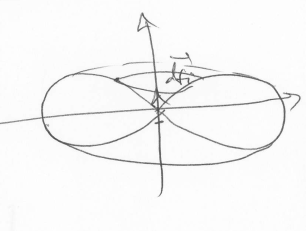
\includegraphics[width=0.5\textwidth]{DiffEm.png}
\end{center}
The total rate for a differential solid angle is given by the interval of this:
\begin{align*}
	W_{fi}^{sp. em} &= \int_{4\pi} \d W_{fi}^{sp.\ em}\\
			&= \frac{\omega_k^3}{8\pi^2\epsilon_0 c^3}
			\int_{4\pi} \d\Omega \left(\abs{\vec{d}_{fi}}^2
			-\abs{\vec{d}_{fi}\cdot\vec{n}}^2\right)\\
			&= \frac{\omega_k^3}{8\pi^2\epsilon_0 c^3}
			\int_{4\pi} \d\Omega \left(\abs{\vec{d}_{fi}}^2
			-(d_{fi})_k(d_{fi})_k n_k n_ell\right)\\
			&= \frac{\omega_k^3}{8\pi^2\epsilon_0 c^3}
			\abs{\vec{d}_{fi}}^2 \left(4\pi - \frac{4\pi}{3}
			\right)\\
	 W_{fi}^{sp. em} &= \frac{\omega_k^3}{8\pi^2\epsilon_0 c^3}
			\abs{\vec{d}_{fi}}^2
\end{align*}

And the intensity (or power) is given by
\[
	I_{fi} = \hslash\omega_{fi}W_{fi}
\]

\subsubsection{Lyman Transitions}
Consider a hydrogen aton in the $2p$ excited state, such that
\begin{align*}
	\psi_i \to \psi_{n,\ell,m} &= R_n(2)iY_{\ell m}(\Omega)\\
	\psi_f \to \psi_{n',\ell',m'} &= R_{n'}(2)iY_{\ell'm'}(\Omega)
\end{align*}
For any $n\to 1$ (ie. from any $n$ value going to $n=1$), we call the
Lyman series
\[
	\vec{d}_{fi} = \int \d^3\vec{x} \psi_{1\ell'm'}(\vec{x})
		\vec{d}\psi_{n\ell m}(\vec{x})
\]
This will all be in the UV spectrum. We call $n = 2 \to 1$ the Lyman-$\alpha$
transition, we call the $n = 3 \to 1$ the Lyman-$\beta$, etc.\\
For any $n\to 2$, we call the Balmer series
\[
	\vec{d}_{fi} = \int \d^3\vec{x} \psi_{2\ell'm'}(\vec{x})
		\vec{d}\psi_{n\ell m}(\vec{x})
\]
This will, finaly, be in the visible range.

\subsubsection{Selection Rules for Electric Dipole Transitions}
We want to look at the matrix elements for the expectation value given by
\[ \brak{f}\vec{x}\bket{i} \to \brak{n',m',\ell'}\vec{x}\bket{n,m,\ell} \]
In order to talk about which of these matrix elements are zero and which are
nonzero, we need to talk about the $\hat{\vec{L}}$ operator:
\begin{align*}
	\hat{\vec{L}}^2 &= \hat{L}_x^2 + \hat{L}_y^2 + \hat{L}_z^2\\
	\hat{\vec{L}}_i &= [\hat{\vec{x}},\hat{\vec{p}}] =
	\epsilon_{ijk}\hat{x}_j\cdot\hat{p}_k
\end{align*}
Recall as well that
\[
	\hat{L}_z\bket{m,\ell} = \hslash m\bket{m,\ell}
\]
We will also need to construct the commutators between the $L$ operator's
components and the $x$ operator's components:
\[
	[\hat{L}_i,\hat{x}_\ell] = i\hslash\epsilon_{i\ell j}\hat{x}_j
\]
Now, we can go back to our question about the matrix elements that we're
looking for, using these relationships:
\begin{align*}
	\brak{m',\ell'}[\hat{L}_i,\hat{x}_j]\bket{m,\ell} &=
	\brak{m',\ell'}i\hslash\epsilon_{i\ell j}\hat{x}_j\bket{m,\ell}\\
	\brak{m',\ell'}\hat{L}_z\hat{x}_j-\hat{x}_j\hat{L}_z\bket{m,\ell} &=
	i\hslash\epsilon_{ijk}\brak{m',\ell'}\hat{x}_k\bket{m,\ell}
	\intertext{Let's first look at the case where $i=z=3$.}
	\hslash m'\brak{m',\ell'}\hat{x}_j\bket{m,\ell} -\hslash
	m\brak{m',\ell'}\hat{x}_j\bket{m,\ell} &=
	i\hslash\epsilon_{ijk}\brak{m',\ell'}\hat{x}_k\bket{m,\ell}\\
	(m'-m)\brak{m',\ell'}\hat{x}_j\bket{m,\ell} &=
	i\epsilon_{zjk}\brak{m',\ell'}\hat{x}_k\bket{m,\ell}\\
	(m'-m)\brak{m',\ell'}\hat{z}\bket{m,\ell} &= 0
\end{align*}
Therefore, for the case $j=z$, we have found our first rule:
\begin{align*}
	m' &= m & \brak{m',\ell'}\hat{z}\bket{m,\ell} &\neq 0\\
	m' &\neq m & \brak{m',\ell'}\hat{z}\bket{m,\ell} &= 0
\end{align*}
Now, let's look at what happens if $j=x,y$ (we'll combine them into a single
set of calculations since we'll find that they just repeat if we do them
individually):
\begin{align*}
	(m'-m)^2\brak{m',\ell'}\hat{x}_j\bket{m,\ell} &=
	(m'-m)i\epsilon_{zjk}\brak{m',\ell'}\hat{x}_k\bket{m,\ell}\\
	(m'-m)^2\brak{m',\ell'}\hat{x}_j\bket{m,\ell} &=
	i\epsilon_{zjk}\epsilon_{zkm}\brak{m',\ell'}\hat{x}_m\bket{m,\ell}\\
	\intertext{We can use the rules for multiplication of Levi-Civita (sp?)
	tensors to simplify this:}
	(m'-m)^2\brak{m',\ell'}\hat{x}_j\bket{m,\ell} &=
	\brak{m',\ell'}\hat{x}_j\bket{m,\ell}\\
	[(m'-m)^2-1]\brak{\ell',m'}\hat{x}_j\bket{\ell,m} &= 0
\end{align*}
So, for $j=x,y$, we get this new set of selection rules:
\begin{align*}
	m' &= m \pm 1 & \brak{m',\ell'}\hat{x}_j\bket{m,\ell} &\neq 0\\
	m' &\neq m \pm 1 & \brak{m',\ell'}\hat{x}_j\bket{m,\ell} &= 0
\end{align*}

Now, let's look at selection rules that involve $\ell$ since we've exhausted
all of the possible $m$ values. To do this, we'll need to know that
\begin{align*}
	[\hat{\vec{L}}^2,\hat{L}_i] &= 0\\
	[\hat{L}_i,\hat{L}_j] &= i\epsilon_{ijk}\hat{L}_k\\
	[\hat{\vec{L}}^2,\hat{x}_j] &=
	2\hslash^2\hat{x}_i+2i\hslash\epsilon_{ijk}\hat{x}_k\hat{L}_j\\
\end{align*}
Note that for this last one, there's a \emph{lot} of algebra, but I don't have
the time to keep up with the lecture right now. I don't think the algebra
itself is particularly important.
Recall also how we can relate these to the $\ell$ index:
\[
	\hat{\vec{L}}^2\bket{m,\ell} = \hslash\ell(\ell+1)\bket{m,\ell}
\]
We now want to look at something real intense:
\begin{align*}
	\left[\hat{\vec{L}}^2,[\vec{\hat{L}}^2,\hat{x}_j]\right] &=
	2\hslash[\hat{\vec{L}}^2,\hat{x}_j] +
	2i\hslash^2\epsilon_{ijk}[\hat{\vec{L}}^2,\hat{x}_k]\hat{L}_j\\
	&= 2\hslash^2[\hat{\vec{L}}^2,\hat{x}_j] + 2i\hslash\epsilon_{ijk}\left(
	2\hslash\hat{x}_k+2i\hslash\epsilon_{mk\ell}\hat{x}_\ell\hat{L}_m\right)
	\hat{L}_j\\
	&= 2\hslash^2[\hat{\vec{L}}^2,\hat{x}_j] + 2i\hslash\left(
		2\hslash\epsilon_{ijk}\hat{x}_k\hat{L}_j -
		2i\hslash\epsilon_{ijk}\epsilon_{m\ell
	k}\hat{x}_\ell\hat{L}_m\hat{L}_j\right)\\
	&= 2\hslash^2[\hat{\vec{L}}^2,\hat{x}_j] + 2i\hslash\left(
		2\hslash\epsilon_{ijk}\hat{x}_k\hat{L}_j -
		2i\hslash(\hat{x}_j\hat{L}_i\hat{L}_j-\hat{x}_i\hat{\vec{L}}^2)
	\right)
	\intertext{There's some simplification here I'm not understanding so
	I'll skip to the end}
	\left[\hat{\vec{L}}^2,[\vec{\hat{L}}^2,\hat{x}_j]\right] &=
	2\hslash^2\left[\hat{\vec{L}}^2\hat{x}_j+\hat{x}_j\hat{\vec{L}}^2\right]
\end{align*}
Now, we can apply this to the transitions we care about to find the selection
rules:
\begin{align*}
	\brak{m',\ell'}2\hslash^2(\hat{\vec{L}}^2\hat{x}_j +
	\hat{x}_j\hat{\vec{L}}^2) &=
	[\hat{\vec{L}}^2,[\hat{\vec{L}}^2,\hat{x}_j]]\bket{m,\ell}\\
	2\hslash^2\left(\hslash^2\ell'(\ell'+1) + \hslash^2\ell(\ell+1)\right)
	\brak{m',\ell'}\hat{x}_j\bket{m,\ell} &= \hslash^{2(?)}
	\left(\hslash\ell'(\ell'+1) - \hslash\ell(\ell+1)\right)^2
	\brak{m',\ell'}\hat{x}_j\bket{m,\ell}\\
	2(\ell'(\ell'+1)+\ell(\ell+1)) \brak{m',\ell'}\hat{x}_j\bket{m,\ell} &=
	(\ell'-\ell)^2(\ell+\ell'+1)^2 \brak{m',\ell'}\hat{x}_j\bket{m,\ell}
\end{align*}
Moving everything to the same side:
\begin{align*}
	\left((\ell'+\ell+1)^2-1-(\ell'-\ell)^2(\ell'+\ell+1)^2\right)
	\brak{m',\ell'}\hat{x}_j\bket{m,\ell} &= 0\\
	\left((\ell'-\ell)^2-1\right)\left((\ell'+\ell+1)^2-1\right)
	\brak{m',\ell'}\hat{x}_j\bket{m,\ell} &= 0
\end{align*}
From this, we can make our $\ell$ selection rules. Assuming that we're not
talking about $\ell=0$ or $\ell'=0$, noting that this works for any $j=x,y,z$:
\begin{align*}
	(\ell'-\ell)^2 &\neq 1 &  \brak{m',\ell'}\hat{x}_j\bket{m,\ell} &= 0\\
	(\ell'-\ell)^2 &= 1 &  \brak{m',\ell'}\hat{x}_j\bket{m,\ell} &\neq 0
\end{align*}
Note that we could re-write $(\ell'-\ell)^2 = 1$ a $\ell' = \ell \pm 1$.
I'm going to just re-write all of the selection rules just to be safe:
\begin{align*}
	m' &= m & \brak{m',\ell'}\hat{z}\bket{m,\ell} &\neq 0\\
	m' &= m \pm 1 & \brak{m',\ell'}\hat{x,y}\bket{m,\ell} &\neq 0\\
	\ell' &\neq \ell \pm 1 &  \brak{m',\ell'}\hat{x}_j\bket{m,\ell} &= 0\\
	\ell' &= \ell \pm 1 &  \brak{m',\ell'}\hat{x}_j\bket{m,\ell} &\neq 0
\end{align*}




\subsubsection{Lifetime of an Excited State}

\section{Scattering and Born Approximations}

\subsection{Classical Scattering Theory}
Let's say we have some object centered on the origin and we send a projectile
towards the object along the $z$ direction. According to Classical theory, the
projectile will hit the object and bounce off in some other direction at an
angle $\theta$ from the $z$ axis, called the scattering angle. We also define
a parameter $b$, called the the impact parameter, which I think represents the
distance of the projectile from the $z$ axis. The question we want to ask
is: what is the dependance of $\theta$ on $b$?\\
In 3 dimensions, let's define an annulus with an inner radius $b$ and a
thickness $\d b$, with a projectile being projected on the differential
azimuthal angle $\d\phi$ (ie. between $\phi$ and $\phi+\d\phi$). The projectile
will be scattered somewhere into the solid angle $\d\Omega$ (composed of
$\d\phi$, the polar angle, and $\d\phi$, the azimuthal angle). We can find two
differential values and combine, using $\sigma$ for cross secion.
\begin{align*}
	\d\sigma &= b\d b\d\phi\\
	\d\Omega &= \sin\theta\d\theta\d\phi\\
	\der{\sigma}{\Omega} &= \text{diff. cross section}
\end{align*}
The total cross section is thus given by
\[
	\sigma = \int_{4\pi}\d\Omega\der{\sigma}{\Omega}
\]

\begin{eg}[Hard-sphere scattering]
\end{eg}

\subsubsection{Impact Parameter}
\subsubsection{Differential Cross Section}
\subsubsection{Scattering on a Sphere}
Let's say we have a bullet that we're shooting at a large, hard ball
with radius $R$, with impact parameter $b$, scatteering angle $\theta$,
and angle $\alpha$ which is one half of the complememntary angle to
$\theta$ (wrong word? The one that's 180-$\theta$. We can thus say
\begin{align*}
	b &= R\sin\alpha\\
	2\alpha+\theta&=\pi\\
	\implies \theta &= \pi-2\alpha\\
	b &= R\sin((\pi-\theta)/2)\\
	  &= R\cos(\theta/2)\\
	\theta &= 2\arccos\left(\frac{b}{R}\right)
\end{align*}
Note that this works as ong as $b\leq R$. For $b>r$, the bullet doesn't
directly hit the ball, so there is no scattering.\\
Now let's look at this in terms of differential cross-section:
\begin{align*}
	\abs{\der{\sigma}{\Omega}} &=
		\abs{\frac{b\d b\d\phi}{\sin\theta\d\theta\d\phi}}\\
	&= \frac{b}{\sin\theta}\abs{\der{b}{\theta}}\\
	&= \frac{R\cos(\theta/2)\frac{R}{2}\sin(\theta/2)}{\sin\theta}\\
	&= \frac{R^2}{4}\frac{2\cos(\theta/2)\sin(\theta/2)}{\sin\theta}\\
	&= \frac{R^2}{4}\\
	\implies \der{\sigma}{\Omega} &= \frac{R^2}{4}\\
	\sigma &= \int_{4\pi}\d\Omega\frac{R^2}{4}\\
	&= \pi R^2
\end{align*}

\subsection{Quantum Scattering Theory}
\subsubsection{Differential Cross-Section}
We're going to use the same picture/setup as before (ie. an annulus projecting
particles at an object between some differential azimuthal angle, towards some
differential solid angle, etc.). Let's define $J_{in}$, the number of
particles throughout $\sigma$ in $1/t$ (also called the incident flux, incident
current density, or the
luminocity). We can define $\d N$, the differential number of particles
recorded in the differentia solid angle $\d\Omega$ per unit time, and to talk
about $\d\sigma$, we will normalize it according to $J_{in}$:
\[
	\d\sigma = \frac{1}{J_{in}}\d N
\]
Such that
\[
	\der{\sigma}{\Omega} = \frac{1}{J_{in}}\der{N}{\Omega}
\]

\subsubsection{Scattering Amplitude}
In quantum, it's often more convenient to operate with waves than with
particles. So let's do that. We can imagine a solid object in a boxwith
propagating waves (eg. a rock in a ripple tank). We'll define the vertical axis
as $x$ and the horizontal axis as $z$ (I don't know why but\ldots here we are).
When the waves hit the rock, they will diffuse circularly around the rock,
propagating outwards. The function that we can use to describe the waves
(assuming they don't change frequency) as
\[
	\psi = e^{ikz} + f(\theta)\frac{e^{ikr}}{\sqrt{r}}
\]
Where the first term represents the plane (initial) waves, and the second term
represents the spherical (scattered) waves, and $f(\theta)$ is the scattering
amplitude. Our goal right now is to find the scattering amplitude. We can
easily generalize this into 3 dimensions:
\[
	\psi = e^{ikz} + f(\theta,\phi)\frac{e^{ikr}}{r}
\]
To test whether or not this is kosher with quantum theory, let's test it with
the Schr\"odinger equation, using $V = V(\vec{r})$ as our potential, which must
be a finite-range potential (ie. must be only active within a range, so no
Coulomb potential):
\[
	\left[-\frac{\hslash^2}{2m}\del^2+V(\vec{r})\right]\psi(\vec{r}) =
		E\psi(\vec{r})
\]
When we're very far away from the scattering center ($r\to-\infty$), if the
potential is a finite-range potential, then we can take $V\to0$ and re-write
the Schr\"odinger equation as
\[
	-\frac{\hslash}{2m}\del^2\psi = E\psi
\]
And simplify:
\begin{align*}
	(\del^2+k^2)\psi &= 0
\end{align*}
Using the magnitude of $k$ that we know,
\[
	k = \frac{\sqrt{2mE}}{\hslash}
\]
Where
\[
	\vec{k} = k\vec{n}
\]
Where $\vec{n}$ is the unit vector in the direcction of $r$.
We will thus write our wave equation solution to this as
\begin{align*}
	\psi = A e^{i\vec{k}\cdot\vec{z}} + Be^{-i\vec{k}\cdot\vec{z}}
\end{align*}
We'll still be discussing waves that are propagating along the $z$ axis, such
that $\vec{k} = k\vhat{e}_z$.\\
Before scattering, the wave equation can be written
\[
	\psi_{in} = e^{ikz}
\]
After scattering, the outgoing wave can be written as
\[
	\psi_{out} = f\frac{e^{ikr}}{r}
\]
The total wave equation must then be
\begin{align*}
	\psi &= \psi_{in} + \psi_{out}\\
	&= e^{ikz} + f(\theta,\phi)\frac{e^{ikr}}{r}
\end{align*}

\subsubsection{Differential Cross Section in terms of f}
We want to find a continuity equation from the Schr\"odinger equation. Remember
that the traditional continuity equation in electrodynamics is
\[
	\pd{t}\rho + (\del\cdot\vec{J}) = 0
\]
Note that we will have to work with the full time-dependent Schr\"odinger
equation here. Recall that density (probability density, in this case) is the
probability density, $\abs{\psi}^2$. Let's try to get the Schr\"odinger
equation in the right form to be able to use $\rho$:
\begin{align*}
	\psi^{\ast}\left(i\hslash\pd{t}\psi\right) &=
	\psi^{\ast}\left(-\frac{\hslash^2}{2m} \del^2\psi \right)\\
	\psi\left(i\hslash\pd{t}\psi^\ast\right) &=
	\psi\left(-\frac{\hslash^2}{2m} \del^2\psi^\ast \right)\\
\end{align*}
If we add these together, we get
\begin{align*}
	i\hslash\pd{t}(\psi\psi^\ast) &= -\frac{\hslash^2}{2m}\left(
	\psi^\ast\del^2\psi + \psi\del^2\psi^\ast\right)
\end{align*}
If we choose to simplify this, noting our previous definition for $\rho$, we
can find the probability current density:
\[
	\vec{J} = -i\frac{\hslash}{2}\left[
		\psi^\ast\del\psi - \psi\del\psi^\ast
	\right]
\]
For the incoming wave, we have
\begin{align*}
	J_{in} &= -i\frac{\hslash}{2m}[ik-(-ik)]\\
	&= \frac{k\hslash}{m}
\end{align*}
For the outcoming wave,
\begin{align*}
	\psi_{out} = f(\theta,\phi)\frac{e^{ikr}}{r}
\end{align*}
So the $\del$ operator will only care about the $r$ component, meaning
\begin{align*}
	J_{out} &= \frac{k\hslash}{m}frac{f f^\ast}{r^2}\\
	&= \frac{k\hslash}{me^2}\abs{f}^2
\end{align*}
Thus, if we say intuitively that $\d N = J_{out} r^2\d\Omega$, then
\begin{align*}
	d\sigma &= frac{r^2J_{out}\d\Omega}{J_{in}}\\
		&= \abs{f}^2\d\Omega\\
	\der{\sigma}{\Omega} &= \abs{f(\theta,\phi)}^2
\end{align*}


\subsubsection{Integral Form of the Schr\"odinger Equation}
If we look at the Schr\"odinger equation,
\[
	\left[-\frac{\hslash}{2m}\del^2+V(\vec{r})\right]\psi(\vec{r}) =
	E\psi(\vec{r})
\]
It's difficult to see a way to be able to easily find $f$. So we want to change
this to make our job a little easier. We can do this by using an inhomogeneous
Helmholtz operator
\[
	\frac{2m}{\hslash^2}
\]
To get an inhomogeneous Helmholtz equation:
\begin{align*}
	\left[\del^2+\frac{2mE}{\hslash^2}\right]\psi(\vec{r}) &=
	-\frac{2m}{\hslash^2}V(\vec{r})\psi(\vec{r})\\
	\left[\del_{r}^2+k^2\right]\psi(\vec{r}) &=
	-\frac{2m}{\hslash^2}V(\vec{r})\psi(\vec{r})
\end{align*}
This equation now describes 2 wave fronts, one moving to the right and one to
the left. Let's try to find the general solution to this, which will be in the
form $\psi(\vec{r}) = \psi_0(\vec{r}) + \tilde{\psi}(\vec{r})$. First, 
\begin{align*}
	[\del_r^2+k^2]\psi_0(\vec{r}) &= 0\\
	\psi_0(\vec{r}) &= Ae^{ikz} + Be^{-ikz}\\
	\psi_0(\vec{r}) &= e^{ikz}
\end{align*}
More difficultly,
\begin{align*}
	[\del_r^2+k^2]\tilde{\psi}(\vec{r}) &=
	-\frac{2m}{\hslash^2}V(\vec{r})\psi(\vec{r})\\
\intertext{This is difficult to solve, but we can make it easier for ourselves
using the Green's function method, making the shift \(\vec{r} \to
	\vec{r}-\vec{r}'\):}
	[\del_r^2+k^2]G(\vec{r}) &= \delta^{(3)}(\vec{r})
\end{align*}
Thus,
\begin{align*}
\tilde{\psi}(\vec{r}) &= \int \d^3\vec{r}'G(\vec{r}-\vec{r}')\left[
	-\frac{2m}{\hslash^2}V(\vec{r}')\psi(\vec{r}')\right]\\
	\text{LHS} &= \int \d^3\vec{r}'[\del_r^2+k^2]G(\vec{r}-\vec{r}')\left[
	-\frac{2m}{\hslash^2}V(\vec{r}')\psi(\vec{r}')\right]\\
\intertext{From the relationship above, we can say then that}
	&= -\frac{2m}{\hslash}V(\vec{r})\psi(\vec{r}) = \text{RHS}
\end{align*}
We need to do a Fourier transformation to deal with the right-hand side of the
equation in order to smooth out the delta function:
\begin{align*}
	\delta^{(3)}(\vec{r}) &= \int\frac{\d^3\vec{q}}{(2\pi)^3}
	e^{i\vec{q}\cdot\vec{r}}\\
	G(\vec{r}) &= \int\frac{\d^3\vec{q}}{(2\pi)^3}
	e^{i\vec{q}\cdot\vec{r}}\tilde{G}(\vec{q})\\
	\text{LHS} &= \int\frac{\d^3\vec{q}}{(2\pi)^3} \left[[\del_r^2+k^2]
	e^{i\vec{q}\cdot\vec{r}}\right]\tilde{G}(\vec{q})\\
	&= \int\frac{\d^3\vec{q}}{(2\pi)^3} \left[[k^2-\vec{q}^2]
	e^{i\vec{q}\cdot\vec{r}}\right]\tilde{G}(\vec{q})\\
	\text{LHS} = \text{RHS} &= \int \frac{\d^3\vec{q}}{(2\pi)^3}
	e^{i\vec{q}\cdot\vec{r}}
\end{align*}
Note that we can do this because of the following properties:
\begin{align*}
	[k^2-\vec{q}^2]\tilde{G}(\vec{q}) &= 1\\
	\tilde{G}(\vec{q}) &= \frac{1}{k^2-\vec{q}^2}
\end{align*}
This is a deceptively complicated integral. To make it easier to solve it,
let's make a transition into spherical coordinates. We will take
\begin{align*}
	\d^3\vec{q} &= q^2\d q\sin\theta\d\theta\d\phi\\
	q_z &= q\cos\theta
\end{align*}
If we do this, then
\begin{align*}
	G(\vec{r}) &= \frac{1}{(2\pi)^3}
	\int_0^\infty\frac{q^2\d q}{k^2-q^2}
	\int_0^{2\pi}\d\phi
	\int_0^\pi\sin\theta\d\theta e^{iqr\cos\theta}\\
	&= \frac{1}{(2\pi)^3}
	\int_0^\infty\frac{q^2\d q}{k^2-q^2}\left(2\pi
	\frac{e^{iqr}-e^{-iqr}}{2qr}\right)\\
	&= \frac{1}{(2\pi)^2}\frac{1}{ir}
	\int_0^\infty\frac{q^2\d q}{k^2-q^2}
	\left[e^{iqr}-e^{-iqr}\right]\\
	&= \frac{1}{i(2\pi)^2r}\int_{-\infty}^{\infty}
	\frac{\d q q e^{iqr}}{k^2-q^2}
\end{align*}
We used antisymmetry rules in that last bit to make it work and change the
limits.\\
We'll define just the integral there as $I_{ret}$. There's a problem: this
integral is not well-defined. That is, it has a pole on the integration axis.
In order to figure out how, we need to look at the complex plane and
use Cauchy's theorem. The option in the complex plane for Cauchy's theorem that
we want to use is the retarded one (as opposed to advanced, etc.)
\begin{center}
	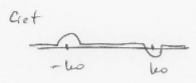
\includegraphics{ret.png}
\end{center}
Just to confirm:
\[
	I_{ret} = \int_{C_{ret}}q\frac{\d q}{k^2-q^2}e^{ikr}
\]
Recall that Cauchy's theorem says that for a closed loop around a pole $z_0$,
\[
	\oint_{z_0}\d z \frac{f(z)}{z-z_0} = 2\pi i f(z_0)
\]
But the contour we've looked at isn't a closed loop. Should we close the loop
above or below the contour? The answer is above. If we try to close it below,
we would find that the way we would have to write the integrand would mean that
it would diverge at $q\to\infty$. So, we close it above, as such:
\begin{center}
	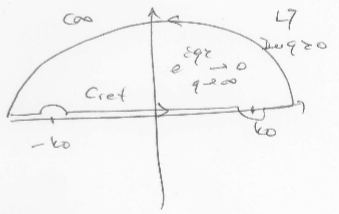
\includegraphics{close_above.png}
\end{center}
If we do this, then
\begin{align*}
	\int{C_{ret}}\frac{\d q q}{k^2-q^2}e^{ikq} &=
	\oint_{C}\frac{\d q q}{k^2-q^2}e^{ikr}\\
	&= 2\pi \res_{q=k} \frac{q e^{ikr}}{(q-k)(k+q)}\\
	&= -2\pi i\frac{ke^{ikr}}{2k}\\
	&= -\pi i e^{ikr}
\end{align*}
Plugging this back into our Green's function, we find that
\[
	G_{ret}(\vec{r}) = -\frac{e^{ikr}}{4\pi r}
\]
This is called a standard Green's function, and it describes an outgoing
spherical wave.
Similarly, had we chosen $G_{adv}$, we would have gotten
\[
	G_{adv} = -\frac{e^{-ikr}}{4\pi r}
\]
We can use either Green's function, or a linear combination of them, but we wan
to use the one which is more intuitive, which is the retarded function.
We can plug this back into the thing we were looking at earlier, the solution
to the Schr\"odinger equation that we needed:
\begin{align*}
	\psi(\vec{r}) &= e^{ikr} - \frac{2m}{\hslash^2}\int\d^3\vec{r}'
	G(\vec{r}-\vec{r}')V(\vec{r}')\\
	&= e^{ikr} - \frac{m}{2\pi\hslash^2}\int\d^3\vec{r}'
	\frac{e^{ik\abs{\vec{r}-\vec{r}'}}}{\abs{\vec{r}-\vec{r}'}} V(\vec{r}')
	\psi(\vec{r}')
\end{align*}
This final equation that we found is called the Lippmann-Schr\"odinger Equation
(or the integral form of the Schr\"odinger equation).

\subsubsection{Asymptotic Form of the Wave Function}

Recall that $\vec{r}'$ is the vector inside of the potential, where the atom is
affected. However, $\vec{r}$ is the vector representing the location of the
detector, far away from $\vec{r}'$, and no longer in the potential. That is,
$\abs{\vec{r}}\gg\abs{\vec{r}'}$. Because of this, we can simplify the second
term in the Lippmann-Schr\"odinger equation by expanding the denominator:
\begin{align*}
	\frac{1}{\abs{\vec{r}-\vec{r}'}}
	&= \frac{1}{\sqrt{(\vec{r}-\vec{r}')^2}}\\
	&= \frac{1}{\sqrt{\vec{r}^2-2\vec{r}\cdot\vec{r}'+\vec{r}'^2}}\\
	&= \abs{\vec{r}}\frac{1}{\sqrt{1-\frac{2\vec{r}\cdot\vec{r}'}{\vec{r}^2}+
	\frac{\vec{r}'^2}{\vec{r}^2}}}\\
\intertext{We can define some \(\epsilon \equiv
\frac{\abs{\vec{r}'}}{\abs{\vec{r}}}\), which is approximately
$\frac{a}{r}\ll1$, so that}
	&= \abs{\vec{r}}\frac{1}{\sqrt{q-\epsilon^1-2\epsilon^2}}\\
	&\approx
	\abs{\vec{r}}\left(1-\frac{\vec{r}\cdot\vec{r}'}{\vec{r}^2}\right)\\
	&= \abs{\vec{r}} - \frac{\vec{r}}{\abs{\vec{r}}}\cdot\vec{r}'\\
	&= \abs{\vec{r}} - \vhat{n}\vec{r}'
\end{align*}
We can use $\vec{k}=k\vhat{n}$ to simplify the exponential to
\[
	e^{ik\abs{\vec{r}-\vec{r}'}} = e^{ik\abs{r}-i\vec{k}\cdot\vec{r}'}
\]
And we can go back to the asymptotic wave function and write 
\begin{align*}
	\psi(\vec{r}) &= e^{ikz} - \frac{m}{2\pi\hslash^2}\frac{e^{ikr}}{r}
	\int d^3\vec{r}'e^{-i\vec{k}\cdot\vec{r}'}V(\vec{r})\psi(\vec{r}')\\
	&= e^{ikz} + f(\theta,\phi)\frac{e^{ikr}}{r}
\end{align*}

\subsection{The Born Approximation}

\subsubsection{The First Born Approximation}
We wrote the Schr\"odinger equation in the form of the Lippman-Schr\"odinger
equation, where it took the form
\[
	\psi(\vec{r}) = \psi_0(\vec{r}) - \frac{m}{2\pi\hslash^2}
	\int\d^3\vec{r}'\frac{e^{ik\abs{\vec{r}-\vec{r}'}}}
	{\abs{\vec{r}-\vec{r}'}}V(\vec{r}')\psi(\vec{r}')
\]
And we look where the obeservation point is very far from the scattering, ie,
$\abs{\vec{r}}\gg\abs{\vec{r'}}$. We also found the asymptotic form of the wave
function, as seen in the last section. Also recall that
\[
	\der{\sigma}{\Omega} = \abs{f(\theta,\phi)}^2
\]
If $V$ is small, then we can use a systematic expansion to try to solve the
asymptotic equation:
\begin{align*}
	0^{th}\text{ order}&: &
	\psi(\vec{x}) &= \psi_0(\vec{x})\\
	1^{st}\text{ order}&: &
	\psi(\vec{x}) &= \psi_0(\vec{x}) + \frac{e^{ikr}}{r}\left(
		-\frac{m}{2\pi\hslash^2}\int d^3\vec{r}'
		e^{-i(\vec{k}\cdot\vec{r}')} V(\vec{r}') \psi_0(\vec{r}')
	\right)
\end{align*}
And so on, but we'll only concern ourselves with the first-order approximation.
Thus, we can write the Born approximation for $f$ as
\[
	f_{Born} = -\frac{m}{2\pi\hslash^2}\int d^3\vec{r}'
	e^{ikr'-i(\vec{k}\cdot\vec{r}')} V(\vec{r}')
\]
We can define some new variables to write
\[
	f_{Born}(\theta,\phi) = -\frac{m}{2\pi\hslash^2}
	\int\d^3\vec{r}' e^{i(\vec{q}\cdot\vec{r}')/\hslash}
	V(\vec{r}')
\]
Note that here, $V$ is not central.
Where
\begin{align*}
	\abs{\vec{q}} &= \hslash\abs{k\vhat{e}_z-\vec{k}}\\
	&= \hslash\sqrt{k^2+k^2-2k(\vhat{e}_z\cdot\vec{k})}\\
	&= \hslash k\sqrt{2(1-\cos\theta}\\
	&= 2\hslash k \sin\left(\frac{\theta}{2}\right)
\end{align*}
In the cae where $V$ is a central potential, that is,
$V(\vec{x}) = V(\abs{\vec{x}}) = V(r')$, we can write this as
\begin{align*}
	f_{Born}(\theta,\phi) &= -\frac{m}{2\pi\hslash^2}
	\int_0^\infty r'^2 \d r'
	\int \d\Omega'e^{iqr'\cos\theta'/\hslash}V(r')\\
	&= -\frac{m}{2\pi\hslash^2} \int_0^\infty
	\d r'(r')^2V(r') 2\pi\int_\pi^02\cos\theta'
	e^{iqr'\cos\theta'/\hslash}\\
	&= -\frac{2m}{q\hslash}\int_0^\infty\d r' r'
	\sin\left(\frac{qr'}{\hslash}\right)V(r')
\end{align*}

\subsubsection{The Validity of the First Born Approximation}
Now that we have this approximation, we needto know how and when this will be
applicable (ie. what restrictions we must impose on $V$ to make this valid). To
determine this, let's not worry about the asymptotic wave function. That is, we
can take $\vec{r} \to 0$. The wave function is thus
\[
	\psi(\vec{r}=0) = 1 - \frac{m}{2\pi\hslash^2}
	\int\d^3\vec{r}'\frac{e^{ik\abs{\vec{r}'}}}
	{\abs{\vec{r}'}}V(\vec{r}')\psi(\vec{r}')
\]
The Born inequality must only be true if the second term is much less than the
first term, so that the wave function doesn't deviate too much from the
incident plane wave. Mathematically,
\[
	1 \gg \abs{
	\frac{m}{2\pi\hslash^2}
	\int\d^3\vec{r}'\frac{e^{ik\abs{\vec{r}'}}}
	{\abs{\vec{r}'}}V(\vec{r}')\psi(\vec{r}')}
\]
In the case of a central potential,
\begin{align*}
	1 &\gg \frac{m}{2\pi\hslash^2}\abs{
	\int_0^\infty\d r' r' \int\d\Omega' e^{ik(r'+r'\cos\theta')}
	V(r')}\\
	1&\gg\frac{m}{k\hslash^2} \abs{
	\int_0^\infty \d r'(e^{2ikr'-q})V(r')}
\end{align*}
Recall that
\[
	k = \frac{\sqrt{2mE}}{\hslash}
\]
In the case of very small (ie. slow) , $ka \ll 1$, and in the case of very
large (ie. fast), $ka \gg 1$. where $a$ is the range of the interaction
potential.\\
For slow particles, where $ka \ll 1$,
\begin{align*}
	1 &\gg \frac{m}{k\hslash^2}\abs{
	\int_0^\infty \d r' V(r') 2ikr'}\\
	&\gg\frac{m}{\hslash^2}\abs{
	\int_0^\infty\d r' V(r')}\\
	1 &\gg \frac{ma^2}{\hslash^2} V
\end{align*}
By extension, and according to the uncertainty principle,
\begin{align*}
	\frac{m}{p^2}V &\ll 1\\
	V &\ll \frac{p^2}{2m} = E_{kin}
\end{align*}
Now, let's look at fast particles, where $ka \gg 1$. We can ignore the term
with the highly oscillating exponential in the inequality, therefore it reads
\begin{align*}
	1 &\gg \frac{m}{k\hslash^2}\abs{
	\int_0^\infty \d r' V(r')}\\
	\intertext{The integral is approximately $aV$, so}
	1 &\gg \frac{ma}{k\hslash^2}\\
	V &\ll \frac{\hslash^2}{ma^2}(ak)\\
	V &\ll \frac{m}{p^2} = E_{kin}(ak)
\end{align*}

\subsubsection{Born Approximation Estimate for the Coulomb Potential}
Recallthat the Coulomb potential is a long-range central potential,
\[
	V(r) = \frac{e^2}{4\pi\epsilon_0}\frac{1}{r}
	\approx \frac{e^2}{4\pi\epsilon_0}\frac{1}{a}
\]
Because it's a long-range potential, we can imagine that we will run into a lot
of problems. But for now, we'll ignore those problems and just use the
equation(s) we found for a short-range potential using the approximation above.
The inequality we found before means that we can write
\[
	1 \gg \frac{m}{k\hslash}\frac{e^2}{4\pi\epsilon_0}
\]
If we multiply and divide by $c$ and shift around the $\hslash$, we can replace
the RH fraction with the fine structure constant. We can also say that
\[
	\frac{k\hslash}{m} = \frac{p}{m} = v
\]
To simplify this immensely and say that
\[
	\frac{v}{c} = \alpha
\]
Recall that $\alpha \approx \frac{1}{137}$.
If we include the $Z$ factor, such that we can say we're looking at a large
object with more particles,
$\frac{v}{c} \gg Z\alpha$, which can quickly blow up. The relativistic
contraction factor, $\gamma = \sqrt{1-(v/c)^2}$ is small in the case of, say,
the hydrogen atom, but will quickly blow up for larger atoms. The Born
approximation thus works for Coulomb potentials for small atoms.

\subsection{Partial Wave Analysis}
\subsubsection{Partial Wave Analysis}
We've discussed only approximate calculations so far for differential cross
sections when the interaction potential is sufficiently small. Now, we're going
to break free from that limitation and solve scattering for arbitrarily-strong
$V$. We will only discuss spherically symmetric potentials, where
$V(\vec{r}) = V(r)$ and $r = \abs{\vec{r}}$. We can separate the variables in
the Schr\"odinger equation using spherical coordinates. Recall that in
spherical coordinates,
\begin{align*}
	\del^2 &= \frac{1}{r}\pd[2]{r}r + \frac{1}{r^2}\del_{\Omega}^2\\
	\del_{\Omega}^2 &= \frac{1}{\sin\theta}\pd{\theta}\sin\theta
		\pd{\theta} + \frac{1}{\sin^2\theta}\pd[2]{\theta}
\end{align*}

The separable form for the solution will be
\[
	\psi(\vec{r}) = R(r) + Y_{\ell m}(\Omega)
\]
With the spherical harmonics obeying the equation
\[
	\del_{\Omega}^2 Y_{\ell m}(\Omega) = -\ell(\ell+1)Y_{\ell m}(\Omega)
\]
So! The Schr\"odinger equation for the radial wave function is, plugging this
in, given by
\[
	-\frac{\hslash^2}{2m}\left[\frac{1}{r}\pd[2]{r}(r R(r)) -
	\frac{\ell(\ell+1)}{r^2} R(r)\right] + V(r)R(r) = ER(r)
\]
As always, we'll ahve to consider only potentials with a finite range of
interaction (ie. $V(r \leq a) \neq 0$, $V(r>a) = 0$). If we do this, we have 3
regions. In order of decreasing $r$, these are:
\begin{enumerate}
\item The far region/radiation region ($V=0$,
		$\frac{\ell(\ell+1)}{r^2} = 0$):
	\begin{align*}
		-\frac{\hslash^2}{2m}\frac{1}{r}\pd[2]{r}(rR(r)) &= ER(r)\\
	\intertext{If we define $U(r) = rR(r)$ and
	$k^2 = \frac{2mE}{\hslash^2}$, then}
		\left(\pd[2]{r} + k^2\right)U(r) &= 0
	\end{align*}
	The solution is clearly
	\begin{align*}
		U_i(r) &= Ae^{ikr} + Be^{-ikr}\\
		R(r) &= A\frac{e^{ikr}}{r} + B\frac{e^{-ikr}}{r}
	\intertext{This describes both an incoming and an outgoing spherical
		wave, but we know that for the scattering case, we only have
	outgoing waves, so $B=0$:}
		R_i(r) &= A\frac{e^{ikr}}{r}
	\end{align*}
\item The intermediate region ($V=0$, $\frac{\ell(\ell+1)}{r^2}\neq 0$)
	\begin{align*}
		-\frac{\hslash^2}{2m}\left[\frac{1}{r}\pd[2]{r}(r R(r)) -
		\frac{\ell(\ell+1)}{r^2} R(r)\right] + V(r)R(r) &= ER(r)\\
		\pd[2]{r}U(r) - \frac{\ell(\ell+1)}{r^2}U(r) + k^2U(r) &= 0
	\end{align*}
	In reality, we can use something like Mathematica for this, but we'll
	solve it analytically for the math. We can start by solving for the
	case $\ell=0$:
	\begin{align*}
		\pd[2]{r}U_0(r) + k^2 U_0(r) = 0
	\end{align*}
	This has solutions, like last time, of
	\begin{align*}
		U_0(r) &= Ae^{ikr} + Be^{-ikr}\\
		R_0(r) &= A\frac{e^{ikr}}{r} + B\frac{e^{ikr}}{r}
	\intertext{In ordr to have a finite $R$ at $r=0$, we must have
	$B=-A$, so that, simplifying a lot,}
		R_0(r) &= \tilde{A}\frac{\sin(kr)}{r}
	\end{align*}
	To solve for $\ell\neq0$, we have to do a bit more work. There's a
	couple ways of doing this, but they all require a \emph{lot} more work,
	so we'll try to brute-force a Rodriguez formula, which won't give us an
	actual answer, but will give us a relationship to be able to work from.
	We need to define our $U$ this time as
	\[
		U_{\ell}(r) = e^{\ell+1}\chi_\ell(r)
	\]
	The second derivative of $U$ is thus
	\[
		\pd[2]{r} U_\ell(r) =
		\ell(\ell+1)r^{\ell-1}\chi_\ell(r) + 2(\ell+1)r^\ell
		\chi'_\ell(r) + r^{\ell+1}\chi''_\ell(r)
	\]
	Such that, going back to the Schr\"odinger equation,
	\[
		\ell(\ell+1)r^{\ell-1}\chi_\ell(r) + 2(\ell+1)r^\ell
		\chi'_\ell(r) + r^{\ell+1}\chi''_\ell(r) - \ell(\ell+1)
		r^{\ell-1}\chi_\ell(r) + k^2r^{\ell+1}\chi_\ell(r) = 0\\
	\]
	Or, simplifying,
	\[
		\chi''_\ell(r) + \frac{2(\ell+1)}{r}\chi'_\ell(r) +
		k^2\chi_\ell(r) = 0
	\]
	If we differentiate this function with respect to $r$, we get
	\[
		\chi'''_\ell(r) - \frac{2(\ell+1)}{r^2}\chi'_\ell +
		\frac{2(\ell+1)}{r}\chi''_\ell(r) + k^2\chi'_\ell(r) = 0
	\]
	If we define $\chi'_\ell(r) = r\phi_\ell(r)$, then
	\begin{align*}
		\chi'_\ell(r) &= r\phi_\ell(r)\\
		\chi''_\ell(r) &= \phi_\ell(r) + r\phi'_\ell(r)\\
		\chi'''_\ell(r) &= 2\phi'_\ell(r) + r\phi''_\ell(r)
	\end{align*}
	Such that
	\begin{align*}
		2\phi'\ell(r) + r\phi''_\ell + \frac{2(\ell+1)}{r}[
		\phi_\ell(r) + r\phi'_\ell(r)] + [k^2 - \frac{2(\ell+1)}{r^2}]
		r\phi_\ell &= 0\\
		r\phi_\ell(r) + 2(\ell+2)\phi'_\ell+rk^2\phi_\ell &= 0A\\
		\phi_\ell(r) + \frac{2(\ell+2)}{r}\phi'_\ell(r) + k^2\phi_\ell
		&= 0
	\end{align*}
	We can see that this is exactly the equation for $\chi_\ell$, with
	$\ell$ shifted by one, so that
	\[
		\phi_\ell(r) = \chi_{\ell+1}(r)
	\]
	Thus, we can relate the two as
	\begin{align*}
		\chi_\ell &= \frac{1}{r}\pd{r}\chi_{\ell-1}\\
		&=
		\frac{1}{r}\pd{r}\left(\frac{1}{r}\pd{r}\chi_{\ell-2}\right)\\
		&= \left(\frac{1}{r}\pd{r}\right)^\ell\chi_0\\
		&= \left(\frac{1}{r}\pd{r}\right)^\ell\frac{\sin(kr)}{r}
	\intertext{Finally, this means}
		U_\ell &= r^{\ell+1}\left(\frac{1}{r}\pd{r}\right)^\ell
		\frac{\sin(kr)}{r}\\
		R_\ell(r) &= A_\ell r^\ell\left(\frac{1}{r}\pd{r}\right)^\ell
		\frac{\sin(kr)}{r}
	\intertext{If we arbitrarily choose $A_\ell=(-1)^\ell/k^\ell$, then we
	can express this in terms of spherical bessell functions. We'll also
	choose $x=kr$ for simplicity.}
		R_\ell(r) &= k(-1)^\ell x^\ell
		\left(\frac{1}{x}\pd{x}\right)^\ell
		\frac{\sin(x)}{x}\\
		&= k j_\ell(x)
	\end{align*}
	Remember that
	\[
		j_\ell(x) = \sqrt{\frac{\pi}{2x}}J_{\ell+1/2}(x)
	\]
	We've now found a solution, but it's not the solution we want. We found
	spherical waves, not standing waves like we'd hoped. Also, we'd have to
	account for the second linearly independent solution to the spherical
	Bessel equations. If we instead define 
	$A_{\ell}^{\pm} = \mp i(-1)^\ell\frac{1}{k^\ell}$, then the solutions
	become
	\[
		R_\ell^\pm(r) = kh_\ell^{(1)}(kr)
	\]
	Where, explicitly, Hankel functions of the first kind are given by
	\[
		h_\ell^{(1)}(x) = -i(-1)^\ell x^\ell\left(
		\frac{1}{x}\pd{x}\right)^\ell\frac{e^{ix}}{x}
	\]
	We can therefore write th solution to the Schr\"odinger equation in the
	intermediate region as
	\begin{align*}
		\psi(\vec{r}) &= \sum_{l=0}^{\infty}\sum_{m=-\ell}^{\ell}
		A_{\ell m}kh^{(1)}(kr)Y_{\ell m}(\theta,\phi)\\
	\intertext{There is no $\phi$ dependence because it's spherically
	symmetric, so $m=0$:}
		&= k\sum_\ell A_\ell\sqrt{\frac{2\ell+1}{4\pi}}h_\ell^{(1)}
		(kr) P_\ell(\cos\theta)
	\end{align*}
	If we define $A_\ell = \sqrt{4\pi(2\ell+1)} i^{\ell+1} a_\ell$, then
	\[
		\psi_{ii}(\vec{r}) =
		k\sum_\ell i^{\ell+1}(2\ell+1)a_\ell h_\ell^{(1)}(kr)
		P_\ell(\cos\theta)
	\]
	For very large $r$, I'm going to skip a lot of the really terrible
	derivations and just write
	\begin{align*}
		\left.h_\ell^{(1)}\right|_{x\to\infty} &=
			(-i)^{\ell+1}\frac{e^{ix}}{x}\\
		\left.\psi_{ii}(\vec{r})\right|_{r\to\infty} &=
			e^{ikr} + f(\theta,\phi)\frac{e^{ikr}}{r}
	\end{align*}
	Where
	\[
		f(\theta,\phi) = \sum_{\ell=0}^\infty
		a_\ell(2\ell+1)P_\ell(\cos\theta)
	\]
	This is the best we can do for now.\\
	But, we can say that the differential an total cross sections are given
	by
	\begin{align*}
		\der{\sigma}{\Omega} &= \abs{f(\theta)}^2\\
		\sigma &= \int_{4\pi}\d\Omega\der{\sigma}{\Omega}\\
		&= \sum_{\ell,\ell'=0}(2\ell+1)(2\ell'+1)a_\ell a^\ast_\ell
		\int_{4\pi}\d\Omega P_\ell(\cos\theta) P_{\ell'}(\cos\theta)\\
		&= 4\pi\sum_{\ell=0}^\infty(2\ell+1)\abs{a_\ell}^2
	\end{align*}
\item The scattering region ($V\neq 0$, $\frac{\ell(\ell+1)}{r^2}\neq 0$)
	We won't actually talk about this right now.
\end{enumerate}

\subsubsection{Determination of Partial Waves}
In ordr to find the partial waves $a_\ell$, we need to solve the Schr\"odinger
equation in the scattering region and sew it with the solution in the
intermediate region using the boundar conditions. The uniform representation
for the wave function in the intermediate region is given by
\[
	\psi(\vec{r}) = e^{ikz} + k\sum_{\ell=0}^\infty a_\ell
	e^{\ell+1}(2\ell+1) h_\ell^{(1)}(kr) P_\ell(\cos\theta)
\]
Where $z=r\cos\theta$. We can write the first term as a linear superposition of
the spherical Bessel function(s), so that
\begin{align*}
	e^{ikz} = e^{ikr\cos\theta} &=
	\sum_{\ell=0}^\infty[A_\ell j_\ell(kr) + B_\ell
	n_\ell(kr)]P_\ell(\cos\theta)\\
	\intertext{On $r\to0$, we must be finite, so $B = 0$:}
	e^{ikr\cos\theta} &= \sum_{\ell=0}^\infty A_\ell j_\ell(kr)
	P_\ell(\cos\theta)
\end{align*}
We can expand each side by a Taylor expansion around
$r\to0$ to find the coefficient $A_\ell$. To do that, we need to
extract the leading power of the RHS when it's expanded with the Rodriguez
formula:
\begin{align*}
	P_\ell(x) &= \frac{1}{2^\ell(\ell!)}\pd[\ell]{x}(x^2-1)^\ell =
	C_\ell x^\ell + \cdots\\
	&= \frac{1}{2^\ell(\ell!)}\pd[\ell]{x}x^{2\ell} + \cdots\\
	&= \frac{1}{2^\ell(\ell!)}\pd[\ell-1]{x}2\ell x^{2\ell-1} + \cdots\\
	&= \frac{1}{2^\ell(\ell!)}\pd[\ell-2]{x}2\ell(2\ell-1)
		x^{2\ell-2} + \cdots\\
	&= \frac{1}{2^\ell(\ell!)}\frac{2\ell(2\ell-1)(\ell+1)\ell x^\ell}
		{(\ell!)} + \cdots\\
	&= \frac{(2\ell)!}{2^\ell(\ell!)^2}x^\ell + \cdots
\end{align*}
Similarly, for $j$:
\begin{align*}
	\left. j_\ell(x) \right|_{x\to 0} &= (-1)^\ell x^\ell
		\left(\frac{1}{x}\pd{x}\right)^\ell \frac{\sin x}{x}\\
	&= (-1)^\ell x^\ell \left(\frac{1}{x}\right)^\ell\frac{1}{x}
		\frac{1}{x}\frac{(-1)^\ell x^{2\ell+1}}{(2\ell+1)!}\\
	&= \frac{x^2}{(2\ell+1)}\left(\frac{1}{x}\pd{x}\right)^\ell x^{2\ell}\\
	&= \left(\frac{1}{x}\pd{x}\right)^{\ell-1}2\ell x^{2\ell-2}\\
	&= \left(\frac{1}{x}\pd{x}\right)^{\ell-2}2\ell(2\ell-2) x^{2\ell-4}\\
	&= \frac{x^2 2\ell(2\ell-2)\ldots2}{(2\ell+1)!}\\
	&= x^\ell\frac{2^\ell \ell!}{(2\ell+1)!}
\end{align*}
So, in total, we can write the expansions of each side as
\begin{align*}
	\sum_{\ell=0}^\infty \frac{i^\ell}{\ell!}k^\ell(r\cos\theta)^\ell &=
	\sum_{\ell=0}^\infty A_\ell\frac{2^\ell \ell!}{(2\ell+1)!}(kr)^\ell
		\frac{(2\ell)!}{2^\ell(\ell!)^2}(\cos\theta)^\ell\\
	\frac{i^\ell}{\ell!} &= \frac{A_\ell}{\ell!}\frac{1}{2\ell+1}\\
	A_\ell &= i^\ell (2\ell+1)
\end{align*}
And thus,
\[
	e^{ikz} = \sum_{\ell=0}^\infty
	i^\ell(2\ell+1)j_\ell(kr)P_\ell(\cos\theta)
\]
and
\[
	\psi_{ii}(\vec{r}) = \sum_{\ell=0}^\infty i^\ell\left[
	j_\ell(kr) + ika_\ell h^{(1)}_\ell(kr)\right] P_\ell(\cos\theta)
\]

\subsubsection{Hard Sphere Scattering}
The potential for thi sphere will be similar to an inifite well, that is,
\[
	V(r) = \begin{cases}
	\infty, & r \leq R\\
	0, & r > R
	\end{cases}
\]
The paricle can't move past the infinite wall, so $\psi_{ii}(r=R)=0$. The wave
function in th eintermediate region is bounded by this boundary condition:
\begin{align*}
	j_\ell(kR) + ika_\ell h^{(1)}_\ell(kR) &= 0\\
	a_\ell &= \frac{i}{k}\frac{j_\ell(kR)}{h^{(1)}(kR)}
\end{align*}
Where the total cross section is
\[
	4\pi\sum_{\ell=0}^\infty\abs{a_\ell}^2(2\ell+1)
\]
On the low energy limit (where $kR \ll 1$), we can find a useful equation of
the total cross section. On this limit,
\begin{align*}
	h^{(1)}(x\to 0) &= i(-1)^\ell x^\ell\left(\frac{1}{x}\pd{x}\right)^\ell
	\frac{e^{ix}}{x}\\
	&+i(-1)^\ell e^{ix} x^\ell \left(\frac{1}{x}\pd{x}\right)^\ell
	\frac{1}{x}\\
	&=i(-1)^\ell e^{ix} x^\ell \left(\frac{1}{x}\pd{x}\right)^{\ell-1}
	\frac{1}{x^3}(-1)\\
	&=i(-1)^\ell e^{ix} x^\ell \left(\frac{1}{x}\pd{x}\right)^{\ell-2}
	\frac{1}{x^5}(-1)(-3)\\
	&= (-1)^\ell e^{ix} x^\ell (-1)^\ell\frac{(2\ell-1)^{2\ell}}{2^\ell
		\ell! x^{2\ell+1}}\\
	&= i e^{ix}\frac{(2\ell)!}{2^\ell \ell!}\frac{1}{x^{\ell+1}}
\end{align*}
Thus, we can write the total cross section as
\begin{align*}
	\sigma &= 4\pi k^{-2} \sum_{\ell=1}^\infty (2\ell+1)
	\abs{\frac{(kR)^\ell2^\ell \ell!}{(2\ell+1)!}
	\frac{2^\ell(\ell!)}{(2\ell)!}(kR)^{\ell+1}}^2\\
	&= 4\pi k^{-2} \sum_{\ell=0}^\infty \frac{(2^\ell
	\ell!)^4}{(2\ell+1)(2\ell!)^4} (kR)^{4\ell+2}\\
\intertext{For the low energy approximation, we can keep only the leading
($\ell=0$) term:}
	&= 4\pi R^2 + \mathcal{O}\left((kR)^6\right)
\end{align*}

\subsection{Phase Shifts}
\subsubsection{Phase Shifts}
We'll start by looking at a simple(r) one-dimensional example. Consider a
one-dimensional plane wave incoming on an infinite wall at $x=0$. Hitting the
infinite wall, the plan wave will reflect, such that the complete wave function
is given by
\[
	\psi(x) = e^{ikx} + A e^{-ikx}
\]
Where the first term represents the incoming, the second represents the
outgoing, and $k=\frac{\sqrt{2mE}}{\hslash}$.
We must have $\psi(x=0) = 0$, which means that $A = -1$, so
\[
	\psi(x) = e^{ikx} - e^{-ikx}
\]
Now, if instead, we have a nonzero potential just before the wall, such that
$V(-a\leq x \leq 0) \neq 0$, the reflected wave function can differ from th
initial by an overal phase. But, by th conservation of probability, we must
still have
\[
	\abs{\psi_{in}}^2 = \abs{\psi_{out}}^2
\]
So if we can write
\[
	\psi_{out} = Ae^{-ikx}
\]
Then this means that $\abs{A}^2 = 1$, and the only possible solution to this is
\[
	A = e^{2i\delta}
\]
Where $2i\delta$ represents the phase shift (and the factor of 2 is just to stay
consistent with the litrature). Thus, the reflected wave function is
\[
	\psi_{out} = e^{-ikx + 2i\delta}
\]
Therefore, the scattering is encoded in the phase.\\
We can extend this back into 3 dimensions. Because of the conservation of
angular momentum, each partial wave scatters independently. For the incoming
plane wave,
\[
	e^{ikz} = \sum_{\ell=0}^{\infty} i^\ell (2\ell+1) j_\ell(kr)
	P_\ell(\cos\theta)
\]
We can take the limit where $r\to\infty$, so that
\[
	j_\ell(x\to\infty) = \frac{1}{2x}\left[
		(-i)^{\ell+1} e^{ix} + i^{\ell+1} e^{-ix}
	\right]
\]
And, by extension,
\begin{align*}
	e^{ikz} &= \sum_{\ell=0}^\infty \frac{i^\ell}{2(kr)}
	(2\ell + 1)P_\ell(\cos\theta) \left[ (-i)^{\ell+1} e^{ikr} +
	i^{\ell+1} e^{-ikr}\right]\\
	&= \frac{1}{2kri} \sum_{\ell=0}^\infty (2\ell+1)P_\ell(\cos\theta)
	\left[e^{ikr} - (-1)^\ell e^{-ikr}\right]
\end{align*}
Thus, for $V=0$,
\[
	\psi = \frac{1}{2kri} \sum_{\ell=0}^\infty (2\ell+1)P_\ell(\cos\theta)
	\left[e^{ikr} - (-1)^\ell e^{-ikr}\right]
\]
We can find $\delta_\ell$ in terms of $a_\ell$ by matching this to a known
expression with $a_\ell$:
\[
	\psi = \frac{1}{2kri} \sum_{\ell=0}^\infty (2\ell+1)P_\ell(\cos\theta)
	\left[j_\ell(kr) + i a_\ell k h_\ell^{(1)}(kr) \right]
\]
Where
\[
	h_\ell^{(1)}(kr)\rvert_{r\to\infty} = (-i)^{\ell+1}
	\frac{e^{ikr}}{kr}
\]
So that, taking $r\to\infty$ for $\psi$, we can find that
\[
	a_\ell = \frac{e^{i\delta_\ell\sin\delta_\ell}}{k}
\]
The sccattering amplitude is
\begin{align*}
	f(\theta) &= \sum_{\ell=0}^\infty (2\ell+1) a_\ell P_\ell(\cos\theta)\\
	&= \frac{1}{k} \sum_{\ell=0}^\infty
	(2\ell+1)e^{i\delta_\ell}\sin\delta_\ell P_\ell(\cos\theta)\\
\intertext{And thus the total cross-section is}
	\sigma &= \frac{4\pi}{k^2}\sum_{\ell=0}^\infty
	(2\ell+1)\sin^2\delta_\ell
\end{align*}
We can compare the forward scattering amplitude (ie., where $\theta=0$) to the
total cross-section to establish a relation between them:
\begin{align*}
	f(\theta=0) &= \frac{1}{k}\sum_{\ell=0}^\infty (2\ell+1)\sin\delta_\ell
	\left[\cos\delta_\ell + i\sin\delta_\ell\right]\\
	\implies \mathrm{Im}[f(\theta=0)] &= \frac{k}{4\pi}\sigma
\end{align*}
This is called the optical theorem, and the phsical origin of theis equation is
the conservation of probability for particles.

\subsection{Scattering from a Delta Function Potential}
Consider a scattering from a spherical delta function potential,
\[
	V(r) = V_0\delta(r-a)
\]
at small velocities (that is, low energies). Find the differential and total
cross-sections.\\
As we found for hard-sphere scattering, we can approximate low energy cross
sections by the $s$ wave contribution, ie.,
\begin{align*}
	\der{\sigma}{\Omega} &= \abs{f_0(\theta)}^2 = \frac{1}{k^2}\sin^2
		\delta_0\\
	\sigma &= \frac{4\pi}{k^2}\sin^2\delta_0
\end{align*}
The only thing we have to do is find the phase shift $\delta_0$. To do this,
we're going to take the Sch\"odinger equation, using the separation of
variables for the solution such that
$\psi(\vec{x}) = r U_\ell(r)Y_{\ell m}(\Omega)$, where $r U_\ell(r) = R(r)$.
Thus,
\[
	\left[ -\frac{\hslash^2}{2m}\pd[2]{r} +
		\frac{\hslash^2}{2m}\ell(\ell+1) + V_0\delta(r-a)
	\right]U_\ell(r) = EU_\ell(r)
\]
On the low-energy limit, where $\ell=0$ (I think that's why we choose $\ell=0$,
at least),
\[
	\left[-\frac{\hslash^2}{2m}\pd[2]{r} + V_0\delta(r-a)\right] = EU_0(r)
\]
Our two boundary conditions are:
\begin{align*}
	r \to 0 &: & \left. R_0(r)\right|_{r\to0} &= \text{Finite}\\
	r \to \infty &: & R(r)|_{r\to\infty} &\to 0\\
\end{align*}
The first boundary condition means that
\[
	U(r\to 0) \to \infty
\]
For the second boundary condition, we need some more space to work. For
$r \neq a$, we have
\[
	\left(\pd[2]{r}-k^2\right)U_0(r) = 0
\]
Where
\[
	k^2 = \frac{2mE}{\hslash^2} > 0
\]
Between 0 and $a$, the solution to this Schr\"odinger equation (which we'll
write as $\overset{<}{U}_0(r)$) is
\begin{align*}
	\overset{<}{U}_0(r) &= A\left(e^{ikr}-e^{-ikr}\right)\\
	&= \tilde{A}\sin(kr)
\end{align*}
Similarly, the solution for $r>a$ is
\[
	\overset{>}{U}_0(r) = \tilde{B}\sin(kr+\delta_0)
\]
We just need to sew these together at $r=a$. We need the function to be
continuous at the boundary, so
\[
	\tilde{A}\sin(ka) = \tilde{B}\sin(ka+\delta_0)
\]
We need a similar condition on the first derivative, which we'll find using the
Schr\"odinger equation, integrating in the vicinity of $r=a$ (that is, between
$a+\epsilon$ and $a-\epsilon$ at the limit $\epsilon\to0$):
\begin{align*}
	\int_{a-\epsilon}^{a+\epsilon}\d r\left[-\frac{\hslash^2}{2m} \pd[2]{r}
	+V_0\delta(r-a)\right]U_0(r) &= E\int_{a-\epsilon}^{a+\epsilon}\d r
	U_0(r)\\
	-\frac{\hslash^2}{2m}\left[\left(\overset{>}{U_0(a)}\right)'
	-\left(\overset{<}{U_0(a)}\right)'\right] + V_0U_0(a) &= 0\\
\end{align*}
The $U$ connected to the potential $V_0$ could really be either of the ones we
found, since we have the condition that they must be the same at $r=a$, but
we'll just arbitrarily pick one of them moving forward:
\begin{align*}
	\left(\overset{>}{U_0(a)}\right)'-\left(\overset{<}{U_0(a)}\right)'&=
	\frac{2mV_0}{\hslash^2}\overset{>}U_0(a)\\
	\tilde{B}k\cos(ka+\delta_0)-\tilde{A}k\cos(ka) &=
	\frac{2mV_0}{\hslash^2}\tilde{B}\sin(ka+\delta_0)\\
	\tilde{B}\left[k\cos(ka+\delta_0)-\frac{2mV_0}{\hslash^2}
	\sin(ka+\delta_0)\right] &= \tilde{A}k\cos(ka)
\end{align*}
If we divide this by our other boundary condition, we find
\[
	k\cot(ka+\delta_0) - \frac{2mV_0}{\hslash^2} = k\cot(ka)
\]
So, as anticipated, when $V_0=0$, $\delta_0=0$ (or multiples of $2\pi$, but 0
is the useful one). When $V_0\neq 0$, however, we need to use our low-energy
approximation ($ka\ll1$):
\[
	k\cot(\delta_0)-\frac{2mV_0}{\hslash^2} \approx \frac{k}{ka} =
	\frac{1}{a}
\]
So that
\[
	\cot(\delta_0) = \frac{1}{ka} + \frac{2mV_0}{\hslash^2k}
\]
So using our low-energy approximations for the differential cross-section,
\begin{align*}
	\der{\sigma}{\Omega} &= \frac{1}{k^2}\sin^2\delta_0\\
	&= \frac{1}{k^2}\frac{1}{1+\cot^2\delta_0}\\
	&= \frac{1}{k^2} \frac{1}{1+\frac{1}{(ka)^2}
	\left[1 + \frac{2mV_0a}{\hslash^2}\right]^2}\\
	&= \frac{a^2}{(ka)^2+\frac{2mV_0a}{\hslash^2}+1}\\
	\sigma &= \frac{4\pi a^2}{(ka)^2+\frac{2mV_0a}{\hslash^2}+1}
\end{align*}

\subsection{Scattering of Identical Particles}

In the case of 1-dimensional identical and indistnguishable, recall that we
cannot write the total wave function of the system as the multiplicative sum of
the individual particles, that is,
\[
	\psi(x_1,\ldots,x_N) \neq \Pi_{i=1}^{N} \psi(x_i)
\]
And recall that we've already seen the [switching] operator, where
\[
	P_{ij}\psi(x_1,\ldots,x_i,\ldots,x_j,\ldots,x_N) =
	\psi(x_1,\ldots,x_j,\ldots,x_i,\ldots,x_N) =
\]
Where squaring the operator gets us back to the original wave function.
Thus, $P^2_{ij} = 1 \implies P_{ij} = \pm 1$. One (+/-) is for bosons, one is
for fermions.\\
Recall that the wave functions for bosons and fermions are given by:
\begin{align*}
	\text{Bosons:}&&
	\psi(x_1,x_2) &= \psi_{n_1}(x_1)\psi_{n_2}(x_2)+
	\psi_{n_1}(x_2)\psi_{n_2}(x_1)\\
	\text{Fermions:}&&
	\psi(x_1,x_2) &= \psi_{n_1}(x_1)\psi_{n_2}(x_2)-
	\psi_{n_1}(x_2)\psi_{n_2}(x_1)\\
\end{align*}
Where bosons have integer spin and a symmetric wf, and fermions have
half-integer spin and antisymmetric wf.

\subsubsection{Scattering of Spin-0 Bosons}
The initial-state wave function for two identical particles approaching each
other at the same speeds on the $z$ axis is
\[
	\psi_{in} = e^{ikz} + e^{-ikz}
\]
After scattering/collision, they will be sent in different directions---one
above axis by the angle $\theta$ and one below at the angle $\pi-\theta$. We
can't necessarily distinguish which one goes in which direction though, if we
put a detector, say, above the axis and wait for something to hit it.\\
The outgoing wave must be symmetric:
\begin{align*}
	\psi_{out} = \frac{e^{ikr}}{r}[f(\theta) + f(\pi-\theta)]
\end{align*}
The differential cross-section is thus
\begin{align*}
	\der{\sigma}{\Omega} &= \abs{f_{sym}}^2\\
	&= \abs{f(\theta)+f(\pi-\theta)}^2\\
	&= \abs{f(\theta)}^2 + \abs{f(\pi-\theta)}^2
	+ 2\mathrm{Re}[f^\ast(\theta)f(\pi-\theta)]
\end{align*}
This differs from the calssical model by the final term, the interference term.

\subsubsection{Scattering of Spin-1/2 Fermions}
The wave function will be written in terms of its spatial and spin coordinates,
ie.,
\[
	\psi(x_1,s_1;x_2,s_2)
\]
Where we have
\begin{align*}
	\abs{\vec{s}} &=  \abs{\vec{s}_1+ \vec{s}_2} = \begin{cases}
	1\\0 \end{cases}\\
	\abs{\vec{s}_1} &= \abs{\vec{s}_2} = \frac{\hslash}{2}
\end{align*}
In the case that the total spin is 0, $\abs{\vec{s}} = 0$,
\[
	\psi(x_1,s_1;x_2,s_2) = X_a(s_1,s_2)\psi_s(x_1,x_2)
\]
Such that spin wave function is antisymmetric, but the spatial one is
symmetric. This is a singlet state, as it's only singly-degenerate (or not
dgenerate? Whatever the terminology is):
\[
	X_a(s_1,s_@) = \frac{1}{\sqrt{2}} \left(\bket{\frac{\hslash}{2}}_1
		\bket{-\frac{\hslash}{2}}_2 - \bket{-\frac{\hslash}{2}}_1
	\bket{\frac{\hslash}{2}}_2\right)
\]
In th case of the total spin being 1, the position is antisymmetric, but the
spin wave function is not, and we have a triplet state, as $s_z$ can now be any
of 1, 0, or -1.
\[
	X_s(s_1,s_2) = \begin{cases}
		\bket{\hslash/2}_1\bket{\hslash/2}_2\\
		\frac{1}{\sqrt{2}} \left(\bket{\hslash/2}_1
		\bket{-\hslash/2}_2 + \bket{-\hslash/2}_1
		\bket{\hslash/2}_2\right)\\
		\bket{-\hslash/2}_1\bket{-\hslash/2}_2
	\end{cases}
\]
Thus, for a singlet state, the differential cross-section is that for the
symmetric wave function, and for the triplet state, for the antisymmetric. If
the incident particle is unpolarized, all states are equally likely, so
\begin{align*}
	\der{\sigma}{\Omega} &= \left.\frac{3}{4}\der{\sigma}{\Omega}\right|_{a}
		+ \left.\frac{1}{4}\der{\sigma}{\Omega}\right|_s\\
	&= \abs{f(\theta)}^2 + \abs{f(\pi-\theta)}^2 -
	\textrm{Re}[f^\ast(\theta)f(\pi-\theta)]
\end{align*}


\section{Quasiclassical (WKB) Approximation}
The WKB approximation is an approximation technique to find solutions to the
Schr\"odinger equation when the quantum system is nearly classical (ie. when
quantum numbers are very very large). In other words, it's treating systems
with slowly verying potentials. We take the point-like limit, when the de
Broglie wavelength $\lambda\to 0$. This approximation will work for us so long
as the real $\lambda$ is much, much smaller than the size of the region we're
looking at along the whole region. This means that in the case of, say, a
positive quadratic potential, this won't work at the turning points.\\
In the case where the potential is flat, we have
\[
	k = \frac{\sqrt{2m(E-V_0)}}{\hslash}
\]
Where $E$ is the energy of the particle and $V$ is the energy of the potential.
In the case where $\hslash\to 0$, $k\to\infty$. The solution to this
Schr\"odinger equation is
\begin{align*}
	\psi = e^{ikx} = e^{ix\sqrt{2m(E-V_0)}/\hslash}
\end{align*}
But what if the potential is not flat? We will write the solution instead in
the still-justifiable form
\[
	\psi = e^{i S(x)/\hslash}
\]
Where $S(x)$ is some complex function. To approximate this classically, we want
to find the expansion of $S(x)$:
\[
	S(x) = S_0(x) + \hslash S_1(x) + \hslash^2 S_2(x) + \cdots
\]
This converges very slowly. The calculation of more than just these first few
leading terms is incredible complicated and we won't really go into it, even
though it only converges slowly. To try to do this, let's start with the
Schr\"odinger equation with a one-dimensional potential, substituting our wave
function:
\begin{align*}
	-\frac{\hslash^2}{2m}\pd[2]{x}\psi(x) + V(x)\psi(x) &= E\psi(x)\\
	-\frac{\hslash^2}{2m}\pd{x}\left[\frac{i}{\hslash}S'e^{iS/\hslash}\right]
		&= E\psi(x)\\
	-\frac{\hslash^2}{2m}\left[\frac{i}{\hslash}S''e^{iS/\hslash}+
	\left(\frac{i}{\hslash}\right)^2(S')^2e^{iS/\hslash}\right]
		&= E\psi(x)\\
	\frac{i}{\hslash}S' + \left(\frac{i}{\hslash}\right)^2(S')^2 +
	\frac{2m}{\hslash^2}(E-V(x)) &= 0\\
	(S')^2 - 2m(E-V(x)) - i\hslash S'' &= 0
\intertext{Substituting the first few terms of th approximation into this, we
get}
	(S_0'+\hslash S_1')^2 - 2m(E-V(x)) - i\hslash(S_0'' +\hslash S_1'')
	&\approx 0\\
	(S_0')^2 + 2\hslash S_0'S_1' - 2m(E-V(x)) - i\hslash S_0'' &\approx 0
\end{align*}
We can separate and align these by powers of $\hslash$:
\begin{align*}
	\hslash^0&:& (S'_0)^2 &= 2m(E-V(x))\\
		 &&&= p^2(x)\\
		 && S'_0 &= \pm p(x)\\
		 && S_0(x) &= \pm \int^x \d x' p(x')\\
	\hslash^1&:& 2S_0'S_1' &= iS_0''\\
		 && S_1' &= \frac{i}{2}\frac{S_0''}{S_0'}\\
		 && S_1 &= \frac{i}{2}\ln(S_0')\\
		 && S_1 &= \frac{i}{2}\ln(p(x))
\end{align*}
There is a missing constant in both of these that we will absorb into the
overall multiplier.\\
Together, the wave function must then be
\begin{align*}
	\psi(x) &\approx e^{i(S_0+\hslash S_1)/\hslash}\\
		&= Ce^{\frac{i}{\hslash}\left(\pm\int^x\d x' p(x') +
		\hslash\frac{i}{2}\ln(p(x))\right)}\\
		&= \frac{C}{\sqrt{p(x)}} e^{\pm\frac{i}{\hslash} \int^x\d x'
		p(x')}
	\intertext{This gives us a linear combination of solutions:}
	\psi(x) &= \frac{A}{\sqrt{p(x)}} e^{\frac{i}{\hslash} \int^x\d x'
		p(x')} + \frac{B}{\sqrt{p(x)}} e^{-\frac{i}{\hslash} \int^x\d x'
		p(x')}
\end{align*}
Where
\[
	\abs{p(x)} = \sqrt{2m(V-E)}
\]
Note that this is only in the classically-allowed region. In the
classically-forbidden region (ie. $E<V$), the signs in the exponentials swap,
and the integrand must take an absolute value.

\subsection{The Applicability of the WKB Approximation}
We said before that this is applicable when $p$ is not small. This means that,
based on the solutions we found, the approximations are valid provided
\[
	\abs{(S')^2} \gg \hslash\abs{S''}
\]
Since $S' = \pm p$ and $p/\hslash = k = 2\pi/\lambda=1/\bar{\lambda}$,
we can write this instead as
\begin{align*}
	\abs{p^2} &\gg \hslash\abs{p'}\\
	1 &\gg \abs{\frac{p'}{p^2}}\\
	1 &\gg \abs{\pd{x}\frac{1}{p}}\\
	1 &\gg \abs{\der{\bar{\lambda}}{x}}
\end{align*}
That is, the wavelength of the particle can change infinitesimale on the
distance scale of order of its size.\\
We can write this condition in terms of $p$ to see what exactly we mean by
``small $p$.'' If
\begin{align*}
	p' &= -\frac{mF}{p}\\
	p &= \sqrt{2m(E-V)}\\
	\implies p' &= -\frac{1}{2} \frac{2m(-V')}{\sqrt{2m(E-V)}} =
	-\frac{mF}{p}
\end{align*}
Then we can write this as
\begin{align*}
	1 &\gg \hslash m \frac{\abs{F}}{p^3}\\
	p &\gg \sqrt[3]{\hslash m\abs{F}}
\end{align*}
We can also make sure the WKB is applicable by using very large quantum
numbers, so that we have a nearly-continuous spectrum of energy levels.

\subsection{Connection Formulas}
Consider a potential well with non-rigid walls. We have two turning points,
$x_1$ and $x_2$, beyond which is the classically-forbidden region, and between
which is the classically allowed region. Our aim is to find the energy levels
in this well. Along the way, we'll also find how to determine the wave function
at the turning points. Note that the WKB applies everywhere in this region
except the turning points.
\begin{align*}
	\intertext{In region I ($x<x_1$):}
	\psi_{I}(x) &= \frac{A}{\sqrt{\abs{p(x)}}} e^{-\frac{1}{\hslash}
	\int_{x}^{x_1}\d x'\abs{p(x')}}
	\intertext{In region II ($x_1<x<x_2$):}
	\psi_{II}(x) &= \frac{B}{\sqrt{\abs{p(x)}}} e^{\frac{i}{\hslash}
	\int_{x}^{x_2}\d x'\abs{p(x')}} +
	\frac{C}{\sqrt{\abs{p(x)}}} e^{-\frac{i}{\hslash}
	\int_{x}^{x_2}\d x'\abs{p(x')}}
	\intertext{In region III ($x>x_2$):}
	\psi_{III}(x) &= \frac{D}{\sqrt{\abs{p(x)}}} e^{-\frac{1}{\hslash}
	\int_{x_2}^{x}\d x'\abs{p(x')}}
\end{align*}
We still need to determine the unknown coefficints. To do this, we have to
connect the 3 regions at the turning points. The problem is, the approximation
fails right at the turning points, so we'd have to solve the Schr\"odinger
equation exactly, at least at first glance. We'll try to avoid that as much as
possible. Instead, we're going to look at another way of doing this. Using
$x_2$ as the first turning point to look at, we can
deform $x$ in the complex plane in order to avoid reaching $x_2$ exactly. We'll
deform it as a circle. We can parameterize $x$ in the complex plane as
\[
	x = x_2 + \rho e^{i\theta}
\]
So we start and end the circular deformation of $x$ at a distance $\rho$ from
$x_2$.
Approaching the region of the turning point, we can use the approximation
\[
	V(x) = V(x_2) + (x-x_2)V'(X_2) + \cdots = E - (x-x_2)F_2 + \cdots
\]
So,
\[
	E - V(x) \approx -(x-x_2)F_2
\]
So the wave function in region III in the vicinity of the turning point is
\begin{align*}
	\psi_{III}(x)|_{x\to x_2} = \frac{D}{\sqrt[4]{2m\abs{F_2}(x-x_2)}}
	e^{-\frac{1}{\hslash} \int_{x^2}^{x_2+\rho e^{i\theta}} \d x'
	\abs{p(x')}}
\end{align*}
Taking a look at just the exponential integral,
\begin{align*}
	I(\rho,\theta) &= \int_{x_2}^{x_2+\rho e^{i\theta}} \d x' \abs{p(x')}\\
	&= \int_{x_2}^{x_2+\rho e^{i\theta}} \d x' \sqrt{2m\abs{F_2}(x-x_2)}\\
	&= \left.\sqrt{2m\abs{F_2}}\frac{2}{3}(x-x_2)^{3/2}\right|_x^2e^{x_2+\rho
	e^{i\theta}}\\
	&= \sqrt{2m\abs{F_2}}\frac{2}{3}\left(\rho e^{i\theta}\right)^{3/2}
	\intertext{The two endpoints of this are at $\theta=0$ and
	$\theta=\pi$:}
	I(\rho,0) &= \sqrt{2m\abs{F_2}}\frac{2}{3}\rho^{3/2}\\
	I(\rho,\pi) &= \sqrt{2m\abs{F_2}}\frac{2}{3}\rho^{3/2}e^{3i\pi/2}\\
	&= -\sqrt{2m\abs{F_2}}\frac{2i}{3}\rho^{3/2}
\end{align*}
$\theta=\pi$ is in region II, so we can stitch it together with those. For
completeness, we'll write
\begin{align*}
	\psi_{III}(x)|_{x\to\x_2, \theta\to\pi} &= \frac{De^{-i\pi/4}}
	{\sqrt{p(x)}}
	e^{\frac{i}{\hslash}\int_x^{x_2}\d x' p(x')}
\end{align*}
This must be equal to the solution in region 2 in the vicinity of the turning
point. When going through the turning point, the asymptotic behavior of the two
region II solutions are vastly different, and it turns out that one becomes
very large and the other very small, so that we can ignore one of them moving
forward. If we ignore the $C$ term, then
\[
	B = De^{-i\pi/4}
\]
But what if we had gone under the axis instead of over? Well, then the opposite
one would be true, and
\[
	C = De^{i\pi/4}
\]
Thus, we find
\begin{align*}
	\psi_II(x) &= \frac{2D}{\sqrt{p(x)}} \left[
	e^{-i\pi/4}e^{i/\hslash\int_x^{x_2}\d x' p(x')}
	e^{i\pi/4}e^{i/\hslash\int_x^{x_2}\d x' p(x')}\right]\\
	&= \frac{2D}{\sqrt{p(x)}}\cos(\frac{1}{\hslash}\int_x^{x_2}\d x' p(x')
	- \frac{\pi}{4}
\end{align*}
Had we done this around the turning point $x_1$ instead, we would have found a
very similar solution:
\[
	\psi_II(x)
	= \frac{2A}{\sqrt{p(x)}}\cos(\frac{1}{\hslash}\int_{x_1}^x\d x' p(x')
	- \frac{\pi}{4}
\]

\subsection{The Bohr-Sommerfeld Quantization Condition}
Since th two solutions in the allowed region have to coincide, the sum of the
phases must be a multiple of $pi$:
\begin{align*}
	\frac{1}{\hslash}\left(
		\int_x^{x_2}+ \int_{x_1}^x
	\right) \d x' p(x') - \frac{\pi}{2} &= n\pi\\
	\frac{1}{\hslash}\int_{x_1}^{x_2} \d x' p(x) &=
	\pi(n+1/2)
\end{align*}
And we also find that
\[
	A = (-1)^n D
\]
We've ignored some terms on the order of $\hslash$.

\subsection{Energy Levels of the Harmonic Oscillator}
The one-dimensional harmonic oscillator has the Hamiltonian
\[
	H = \frac{p^2}{2m} + \frac{m\omega^2}{2}x^2
\]
So the momentum is
\[
	p(x) = \sqrt{2m - m^2\omega^2x^2}
\]
The turning points (ie. where $p=0$) are where $E=V$, or where
\[
	E = \frac{m\omega^2}{2}x^2
\]
So, the two turning points are
\begin{align*}
	x_+ &= \sqrt{\frac{2E}{m\omega^2}}\\
	x_- &= -\sqrt{\frac{2E}{m\omega^2}}
\end{align*}
So using the Bohr-Sommerfeld quantization condition.
\begin{align*}
	\frac{1}{\hslash}\int_{x_-}^{x_+} \d x'
	\sqrt{2m(E-m\omega^2x^2/2)} &= \pi(n+1/2)\\
	m\omega\frac{1}{\hslash}\int_{x_-}^{x_+} \d x'
	\sqrt{2E/(m\omega^2) - x'^2} &= \pi(n+1/2)\\
	m\omega\frac{1}{\hslash}\int_{x_-}^{x_+} \d x'
	\sqrt{x_+^2 - x'^2} &= \pi(n+1/2)\\
	\intertext{If we define $x'=x+y$, then}
	m\omega\frac{1}{\hslash}\int_{x_-}^{x_+} \d x'
	\sqrt{1-y^2} &= \pi(n+1/2)\\
\end{align*}
I won't go through the exact derivation, but it's simple to prove that
the integral is simply $\pi/2$. Skipping some basic agebra simplification,
\begin{align*}
	E = \hslash\omega\left(n+\frac{1}{2}\right)
\end{align*}
In this case, it reproduces the exact energy levels. This is an exception, but
it is a pretty cool exception.

\subsection{Bound States in the Potential with One Rigid Wall}
Consider a particle in the potential $V(x)$ with a single infinite wall at
$x=x_1$. To findthe energylevels in it (ie. the quantization condition), we
have to find the expansion for the WKB wave function in the domain
$x_1<x<x_2$, where $x_2$ is the turning point, by going through the turning
points on the left and the right, as below:
\begin{center}
	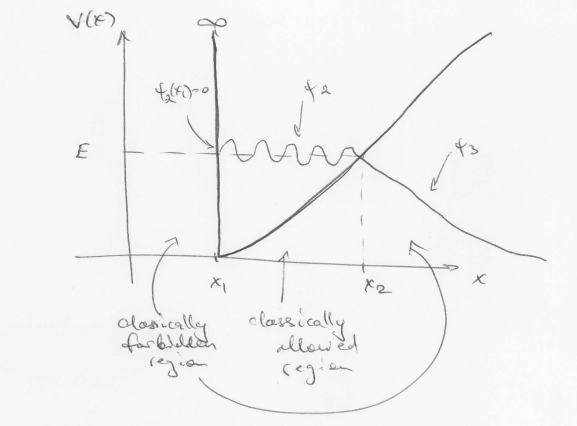
\includegraphics[width=.5\textwidth]{OneWall.png}
\end{center}
We found before that generaically, in the range $x<x_2$,
\begin{align*}
	\psi_{III}(x) &= \frac{D}{\sqrt{\abs{p}}} e^{
	-\frac{1}{\hslash}\int_{x_2}^x\d x\abs{p(x')}}
\intertext{And in the range $x_1<x<x_2$,}
	\psi_{II}(x) &= \frac{2C}{\sqrt{p(x)}} \cos\left(
	\frac{1}{\hslash}\int_x^{x_2}\d x' p(x')-\frac{\pi}{4}\right)\\
	\psi_{II}(x) &= \frac{2C}{\sqrt{p(x)}} \cos\left(
	\frac{1}{\hslash}\int_{x_1}^x\d x' p(x')+\alpha\right)\\
\end{align*}
The only difference now is the boundary condition at $x_1$, where the solution
for $x<x_1$, $\psi_I(x) = 0$ since the wall is infinitely large. We can match
either of the above solutions at $x=x_1$, but we'll choose the one that already
involves $x_1$:
\begin{align*}
	0 &= \frac{2C}{\sqrt{\abs{p(x)}}}\cos(\alpha)\\
	\alpha &= -\frac{\pi}{2} + m\pi
\end{align*}
where $m$ can be positive or negative odd integers. If we add the two
$psi_{II}$ wave functions together to try to find the full wave function in the
classically-allowed region, we find that
\begin{align*}
	\frac{1}{\hslash}\int_{x_1}^{x_2} \d x' p(x') =
	\pi\left(n+\frac{3}{4}\right)
\end{align*}

\subsection{Bound States in the Potential with Two Rigid Walls}
In the case that we have two rigid walls, we the solution is pretty simple.
Now, in the classically-forbidden region, we have $\psi_1 = \psi_3 = 0$, and in
the classically-allowed region, we can have an arbitrarily-complex potential.
Matching at $x = x_2$ and $x=x_1$, we find that the phase shift for both is
$-\frac{\pi}{2}$, so we can write
\[
	\frac{1}{\hslash} \int_{x_1}^{x_2} \d x' p(x') =
	\pi(n+1)
\]

\subsection{Tunneling through a Potential Barrier}

Nowe we'll be looking at the opposite of a potential well. COnsider a potential
barrier with square walls and a bumpy top. The limitation of the current
consideration of square wlls is for the sake of simplification, so that we can
have clearly-defined classically allowed and forbidden regions.
\begin{center}
	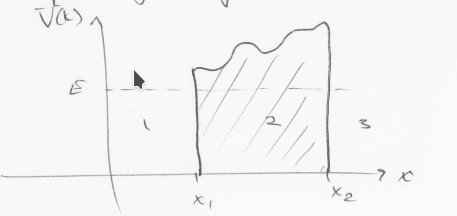
\includegraphics[width=.6\textwidth]{Tunnelling_WKB.png}
\end{center}
In the region $x<x_1$, we have both an incoming and outgoing wave. Remembering
that we can define $k=\sqrt{2mE}$, we can write the wave function in region I
as
\[
	\psi_I(x)  = Ae^{ikx} + Be^{-ikx}
\]
In the region $x>x_2$, we similarly have a free wave function, but this time
only a transmitted wave, with the wave function
\[
	\psi_{III}(x) = F^{ikx}
\]
Finally, we need to look in the region $x_1<x<x_2$. In the WKB approximation,
\[
	\psi_{II}(x) = \frac{C}{\sqrt{\abs{p(x)}}} e^{-\frac{1}{\hslash}
	\int_{x_1}^x\d x'\abs{p(x)}} +
	\frac{D}{\sqrt{\abs{p(x)}}} e^{\frac{1}{\hslash}
	\int_{x_1}^x\d x'\abs{p(x)}}
\]
When the barrier becomes infinitly wide ($x\to\infty$), the second of these
grows exponentially, and we need a normalizable wave function, so we can call
this unphysical and say $D=0$, so what we're left with is
\[
	\psi_{II}(x) = \frac{C}{\sqrt{\abs{p(x)}}} e^{-\frac{1}{\hslash}
	\int_{x_1}^x\d x'\abs{p(x)}}
\]
We can write the transmission/tunneling probability as
\[
	T = \frac{\abs{F}^2}{\abs{A}^2}
\]

Our goal is to find $F$ in terms of $A$ by relating them through $C$. We can
sew the solutions at $x_1$ and $x_2$. We're going to ignore the pre-factors a
little bit to make our lives a little easier. So we'll look just at the leading
terms. Matching the wave functions and their derivatives at $x=x_1$,
\begin{align*}
	Ae^{ikx_1} + Be^{-ikx_1} &= C\\
	ikAe^{ikx_1} - ikBe^{-ikx} &= aC\\
	Ae^{ikx_1} - Be^{-ikx_1} &= \tilde{a}C\\
	\intertext{If  we add this third line to the first line, we find}
	\abs{2Ae^{ikx_1}} &= {(1+\tilde{a})C}\\
	\abs{A} &\propto \abs{C}
\end{align*}
Now, matching at $x_2$,
\begin{align*}
	Ce^{-\frac{1}{\hslash}\int_{x_1}^{x_2}\d x'\abs{p(x')}} &=
	\abs{Fe^{ikx_2}}\\
	\abs{C}e^{-\frac{1}{\hslash}\int_{x_1}^{x_2}\d x'\abs{p(x')}} &=
	\abs{F}\\
\end{align*}
Therefore, the leading WKB result for the transmission probability is
\begin{align*}
	T &\propto e^{-2\gamma}\\
	\gamma &= \frac{1}{\hslash}\int_{x_1}^{x_2}\d x'\abs{p(x')}
\end{align*}

\subsection{Cold Emission of Electrons from Metal}
Consider a chunk of metal with free-to-move electrons inside of it. The
potential for the electrons should be a step function, such that the electrons
are free inside, but face some barrier (at the size of the work function $V_0$)
to get out:
\[
	V(x) = \begin{cases}
		V_0, & x>0\\
		0,   & x<0
	\end{cases}
\]
If we turn on an electric field $\mathcal{E}$
outside the metal, a force will be exerted
on the electrons with magnitude $F=e\mathcal{E}$
(assuming there's no electric field inside the metal). For $x>0$, we now have
$V(x) = V_0-e\mathcal{E}x$.
The barrier now looks like this:
\begin{center}
	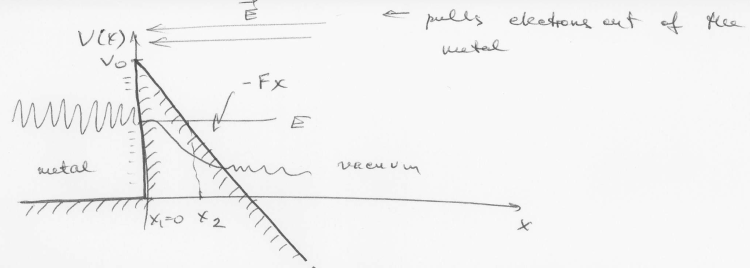
\includegraphics[width=\textwidth]{E_WKB.png}
\end{center}
The electrons are now able to tunnel out through the barrier. $x_1=0$, and
we can find $x_2$ by discovering where the energy of the electron is equal to
the value of the potentialm or $x_2 = \frac{V_0-E}{e\mathcal{E}}$.
Now, we just need to calculate $\gamma$:
\begin{align*}
	\gamma &= \frac{1}{\hslash}\int_0^{\frac{V_0-E}{e\mathcal{E}}}\d x'
	\sqrt{2m(V_0-E-e\mathcal{E}x)}\\
	&= \frac{\sqrt{2me\mathcal{E}}}{\hslash}
	\int_0^{\frac{V_0-E}{e\mathcal{E}}}\d
	x'\sqrt{\frac{V_0-E}{e\mathcal{E}} - x}\\
	&= \left.\frac{\sqrt{2me\mathcal{E}}}{\hslash}\frac{2}{3} \left(
		\frac{V_0-E}{e\mathcal{E}}-x
	\right)\right|_{0}^{\frac{V_0-E}{e\mathcal{E}}}\\
	&= \frac{2}{3}\frac{\sqrt{2m}}{\hslash e\mathcal{E}}(V_0-E)^{3/2}
\end{align*}
So that the probability of tunneling out of the metal is
\[
	T \propto e^{-\frac{4}{3}\frac{\sqrt{2m}}{\hslash e\mathcal{E}}
	(V_0-E)^{3/2}}
\]
This is used in scanning tunneling microscopes to construct accureate maps of
the suface under investigation. This is the end of what will be covered on the
exams.

\section{Berry's Phase}
\subsection{Nonholonomic Process}
Onsider a pendulum mounted on a ball and moved around a closed path. Like,
let's say you and some friends on another continent  asked Santa for a pendulum
for Christmas.
\begin{center}
	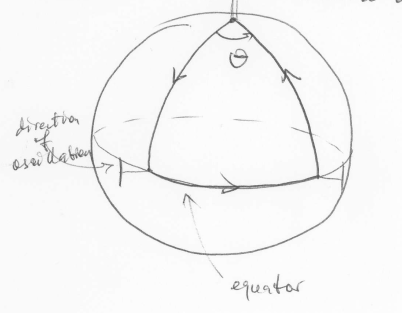
\includegraphics[width=0.5\textwidth]{santa.png}
\end{center}
It's hard to see from the picture, but if the direction of the pendulum is
originally in the direction of the first path, when we return to the starting
point, it will be in the opposite direction---that is, in the direction of the
third path. More generally, it will have changed such that the planes of
oscillation are separated by some angle $\theta$.
This is an example of a nonholonomic process. Note that this only
works for a slow path. That means that we can talk about this in the same way
we talked about things in the Adiabatic approximation.\\
The angle $\theta$ is equal to the solid angle $\Omega$ subtended by the path.
Recall that
\[
	\d\Omega = \d\phi\sin\vartheta\d\vartheta
\]
For us,
\[
	\Omega = \int_0^\theta\d\vartheta\int_0^{\pi/2} \d\vartheta
	\sin\vartheta =	\theta
\]
This is a nice result becaue it doesn't depend on the shape of the path.

\subsection{Geometric Phase}
According to the Adiabatic theorem, a particle that starts in the $n^{th}$
eigenstate of $\hat{H}(t)$ at $t=0$ remains in it at $t>0$:
\[
	\psi_n(t) = \psi_n(0)e^{-i\Theta_n(t) + i\gamma_n(t)}
	\psi_n(t)
\]
With the dynamic phase being
\[
	\Theta_n(t) = \frac{1}{\hslash}int_0^t\d t' E_n(t')
\]
And the geometric phase being
\[
	\gamma_n(t) = -\int_0^t\d t'
	\braket{\psi_n(t')}{\dot{\psi}_n(t')}
\]
If the Hamiltonian is time-dependent, it has some factor in it $\vec{x}(t)$,
such that $\bket{\psi_n(t)} = \bket{\psi_n(\vec{x}(t))}$, and therefore
\[
	\pd{t}\bket{\psi_n(t)} = \der{\vec{x}}{t} \cdot \del
	\bket{\psi_n\left(\vec{x}(t)\right)}
\]
So we can write the geometric phase as
\begin{align*}
	\gamma_n(t) &= \int_{\vec{x}(0)}^{\vec{x}(t)}\d\vec{x}\cdot
	\braket{\psi_n}{\del\psi_n}
\intertext{We can often write this in terms of a constant, so that}
	\gamma_n(t) &= \int_{\vec{x}(0)}^{\vec{x}(t)}\d\vec{x}\cdot
	\vec{A}(\vec{x})
\end{align*}
If the Hamiltonian refers to the same form at $t=T$ as it did at $t=0$, the
geometric phase doesn't vanish (but I think it does any other time), and
\begin{align*}
	\gamma_n(T) &= i\oint\d\vec{x} \cdot \braket{\psi_n}{\del\psi_n}\\
	&= i\int_S\d\vec{S} \cdot \left[\del\times\vec{A}\right]\\
	\intertext{This looks a lot like a flux through a magnetic
	induction---it's not really, but we'll write it like it is}
	&= i\int\d\vec{S} \cdot \vec{B}
\end{align*}
Note that this depends only on the path taken, not on how fast it's transversed
(ie. there's no explicit time-dependence). This gamma in this form is known as
Berry's phase (where the $\vec{B}$ comes from).
Note that to make this happen, we've had to define a ``magnetic field'' as
\[
	\vec{B} = \del\times\braket{\psi_n}{\del\psi_n}
\]

\subsubsection{Electron in a Slowly Changing Magnetic Field}
Let' discuss the problem of a magnetic moment $\vec{\mu}$ in a time-varying
magnetic field $\vec{B}(t)$.
We can define the field very basically below
\begin{center}
	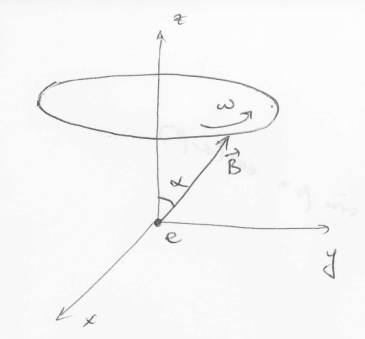
\includegraphics[width=0.5\textwidth]{BerrysField.png}
\end{center}
Where there is two types of procession, with
\begin{align*}
	\omega &= \abs{\vec{\omega}}\\
	\vec{\omega} &= \omega\vhat{z}\\
	\vec{\omega}_B &= \omega_B\frac{\vec{B}}{\abs{\vec{B}}}
\end{align*}
We can write $\vec{B}$, using the restriction that $\abs{\vec{B}} = B_0$, as
\[
	\vec{B(t)} = B_0 \left( \sin\alpha\cos(\omega t), \sin\alpha\sin(\omega
	t), \cos\alpha \right)
\]
The Hamiltonian is defined by
\begin{align*}
	H &= \vec{\mu}\cdot\vec{B}\\
	&= \frac{e}{m}\vec{B}\cdot\vec{S}\\
	&= \frac{e\hslash}{2m}\vec{\sigma}\cdot\vec{B}(t)A\\
	&= \frac{e\hslash B_0}{2m}\begin{pmatrix}
		\cos\alpha & \sin\alpha e^{-i\omega t}\\
		\sin\alpha e^{i\omega t} & -\cos\alpha
	\end{pmatrix}
\end{align*}
In order to write this whole thing as a linear algebra problem, we'll have to
define
\[
	\psi = \begin{pmatrix} a\\b \end{pmatrix}
\]
So the Schr\"odinger equation is
\begin{align*}
	\frac{\hslash}{2}\frac{eB_0}{m}
	\begin{pmatrix}
		\cos\alpha & \sin\alpha e^{-i\omega t}\\
		\sin\alpha e^{i\omega t} & -\cos\alpha
	\end{pmatrix}
	\begin{pmatrix}
		a\\
		b
	\end{pmatrix}
	 &= E
	\begin{pmatrix}
		a\\
		b
	\end{pmatrix}
\end{align*}
We can diagonalize the matrix here, calling it $M = UDU^\dagger$, where $D$ is
a diagonal matrix with elements corresponding to $M$'s eigenvalues, which we'll
call $d_1$ and $d_2$. We know that $\det(M) = -1$, so
\[
	\det(UDU^\dagger) = \det(D) = d_1d_2 = -1
\]
Which gives us the solutions
\begin{align*}
	E &= \pm\frac{\hslash}{2} \frac{eB_0}{m}\\
	&= \frac{\hslash\omega_B}{2}\\
	\omega_B &= \frac{eB_0}{2}
\end{align*}
Now, we need to solve the matrix equation
\begin{align*}
	\begin{pmatrix}
		\cos\alpha & \sin\alpha e^{-i\omega t}\\
		\sin\alpha e^{i\omega t} & -\cos\alpha
	\end{pmatrix}
	\begin{pmatrix}
		a\\
		b
	\end{pmatrix}
	 &=
	\begin{pmatrix}
		a\\
		b
	\end{pmatrix}
\end{align*}
This is not super difficult and we'll skip the full derivation to just get the
answers (note that there's 2, one for each of the eigenvalues):
\begin{align*}
	\psi_+ = \begin{pmatrix} a_+\\b_+ \end{pmatrix} =
	\begin{pmatrix}
		\cos\frac{\alpha}{2}\\
		\sin\frac{\alpha}{2}\ e^{i\omega t}
	\end{pmatrix}
	\psi_+ = \begin{pmatrix} a_-\\b_- \end{pmatrix} =
	\begin{pmatrix}
		\sin\frac{\alpha}{2}\ e^{-i\omega t}\\
		-\cos\frac{\alpha}{2}
	\end{pmatrix}
\end{align*}
We now need to find the solution to the time-dependent Schr\"odinger equation,
where we'll write
\[
	\psi(t) = C_+(t)\psi_+(t) + C_-(t)\psi_-(t)
\]
We can define a vector $\vec{\lambda} = \vec{\omega}-\vec{\omega}_B$, such that
\[
	\abs{\vec{\lambda}} = \lambda =
	\sqrt{\omega^2 + \omega_B^2 - 2\omega\omega_B\cos\alpha}
\]
When we can (skipping a few steps that are calculatable in, say, Mathematica or
something) say that
\begin{align*}
	C_+(t) &= \left[\cos\frac{\lambda t}{2} -
		i\frac{\omega_B-\omega\cos\alpha}{\lambda}
		\sin\frac{\lambda t}{2}\right]
		e^{i\omega t/2}\\
	C_-(t) &= i\frac{\omega}{\lambda}\sin\alpha
		\sin\frac{\lambda t}{2} e^{i\omega t/2}
\end{align*}
In the adiabatic assumption, $\omega \ll \omega_B$, meaning that
\begin{align*}
	\lambda &\approx \omega_B - \omega\cos\alpha\\
	C_- &\approx 0\\
	C_+ &\approx e^{-i\omega_B t/2} e^{-i\omega t(1-\cos\alpha)/2}\\
	    &= e^{i\Theta(t)}e^{\gamma(t)}
\end{align*}
Such that
\[
	\gamma(t) = -i\frac{\omega t}{2} (1-\cos\alpha)
\]
For a complete processional cycle, as below, we can find that
\[
	\gamma(T) = -i\pi(1-\cos\alpha)
\]
\begin{center}
	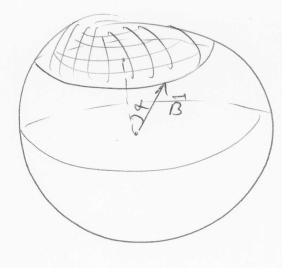
\includegraphics[width=0.5\textwidth]{BerrysField1.png}
\end{center}
In doing this, more generally, we took the solid angle,
\[
	\Omega = \int_0^{2\pi}\d\phi\int_0^\alpha\d\theta\sin\theta
		= 2\pi(1-\cos\theta)
\]
So it is equally accurate to write
\[
	\gamma_+(T) = \frac{1}{2}\Omega
\]

But let's take it more generally---what if the procession wasn't solid like
that, as in the path below:
\begin{center}
	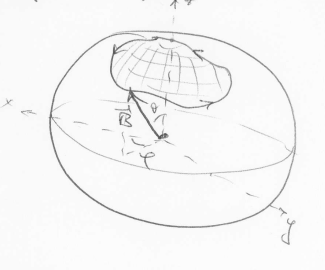
\includegraphics[width=0.5\textwidth]{BerrysField2.png}
\end{center}
We have a problem: we don't know the form of $\vec{B}$. So how can we solve it?
Well, let's use Berry's phase, because that'll tell us a lot. We know that
generally,
\begin{align*}
	\gamma(T) &= i\oint_C\d\vec{x} \cdot \braket{\psi_+}{\del\psi_+}\\
	&= i\int_S\d\vec{S} \left[\del\times\vec{A}\right]
\end{align*}
We need to find $\vec{A}$, considering $\alpha$ as the generic polar angle
$\theta$, and $\omega t$ as our azimuthal angle $\phi$. We know $\vec{A}$ from
our definition, which we'll mildly re-write as
\[
	\vec{A} = \psi_+^\dagger \del\psi_+
\]
and $\psi_+$ from earlier in this section, and we know that in
spherical coordinates,
\[
	\del = \vhat{r}\pd{r} + \frac{1}{r}\vhat{\theta}\pd{\theta} +
	\frac{1}{r\sin\theta}\vhat{\phi}\pd{\phi}
\]
The radius isn't changing, so that term will go to 0, and we can write
$\vec{A}$, skipping the simplification, as
\begin{align*}
	\vec{A} &= \vhat{\phi}\frac{i}{2r}\tan\frac{\theta}{2}
\end{align*}
The curl of $\vec{A}$ is thus (again, I'm not going to do the simplification,
this is super possible on my own with just some trig tricks)
\[
	\frac{i\vhat{r}}{2r^2}
\]
So, going back to the very beginning, this means that we can write
\begin{align*}
	\gamma(T) &= -\frac{1}{2}\int_\Omega\d \Omega\\
		  &= -\frac{1}{2}\Omega
\end{align*}

\subsection{The Aharamov-Bohm Effect}
The Berry's phase has measureable physical consequences. A typical setup to
measure this is the following:

The signal we detect will be a linear superposition of the original and the
Berrry's phase-shifted wave functions,
\begin{align*}
	\abs{\tilde{\psi}}^2 = \frac{1}{4}\abs{\psi}^2\abs{1+e^{i\gamma}}^2
	= \abs{\psi}^2\sin\left(\frac{\gamma}{2}\right)^2
\end{align*}

\subsubsection{Particle in the Vicinity of a Solenoid}
We've already discussed that in an electromagnetic field, the Hamiltonian is
written in terms of $\vec{A}$ and $\phi$, rather than $\vec{E}$ and $\vec{B}$,
\[
	\hat{H} = \frac{1}{2m}\left(\vhat{p}-q\vhat{A}\right)^2 + q\phi
\]
But also recall that the theory is gauge-invariant, so we can make the
transformation
\begin{align*}
	\vec{A} &\to \vec{A}' = \vec{A} + \del\chi\\
	\phi &\to \phi'  \phi - \pd{t}\chi
\end{align*}

Aharamov and Bohm showed that the vector potential can affect the quantum
behavior of a charged particle even when it is moving through a vanishing
field.\\
We'll take a look at an example with a charged oarticle near an infinitely-long
solenoid with current $I$. The magnetic field inside of the solenoid is
uniform, and we expect it to be $0$ on the outside. We can find a more exact
solution by integrating the following expression over the section of the
solenoid subtended by a circular contour of radius $r$:
\begin{align*}
	\int_S \d\vec{S}\cdot\del\times\vec{A} &= \int_S\d\vec{S} \vec{B}\\
	\oint_C\d\vec{r}\cdot\vec{A} &= \\abs{\vec{B}}\pi a^2\
	2\pi r \abs{\vec{A}} &= \Phi\\
	\abs{\vec{A}} &= \frac{\Phi}{2\pi r}
\end{align*}
We can also find that, due to the directional necessity of the curl
\[
	\del\times\vec{A} = \vec{B}
\]
$\vec{A}$ must be in the direction $\vhat{\phi}$.
The solenoid itself is uncharged, so $\phi=0$, meaning we can re-write the
Hamiltonian as
\[
	\hat{H} = \frac{1}{2m}\left[-i\hslash\del - \frac{q\Phi}{2\pi
	r}\vhat{\phi}\right]^2
\]
Note that the $\phi$ direction is the only thing that's
changing in this, so we can replace $\del$ with
$\frac{\vhat{\phi}}{r}\pd{\phi}$, and use this in the
Schr\"odinger equation:
\begin{align*}
	\frac{1}{2m}\left[-\frac{i\hslash}{r}\pd{\phi} -
	\frac{q\Phi}{2\pi 4}\right]^2\psi(\phi) &= E\psi(\phi)
\end{align*}
We can write the sollution to this, very generally, as
\[
	\psi(\phi) = A_+ e^{i\lambda+\phi} + A_-e^{-i\lambda-\phi}
\]
So we can plug in and simplify, to find that
\begin{align*}
	\frac{1}{2m}\left[\frac{\hslash\lambda}{r} - \frac{q\Phi}{2\pi r}
	\right]^2 &= E\\
	\sqrt{\left[\lambda-\frac{q\Phi}{2\pi\hslash}\right]^2} &= \pm
		\sqrt{\frac{2mEr^2}{\hslash^2}}\\
	\lambda_{\pm} &= \frac{q\Phi}{2\pi\hslash} \pm
		\frac{r}{\hslash}\sqrt{2mE}
\end{align*}
We also have a boundary condition (of sorts), that
\[
	\psi(\phi) = \psi(\phi+2\pi)
\]
So that we should be able to replace $\phi$ with $\phi+2\pi$ at any point
without changing anything. To stay consistent with the literature, it is common
to re-write $A_\pm$ as $n$ (which makes sense if we do the algebra of the above
equality), so that
\[
	n = \frac{q\Phi}{2\pi\hslash} \pm \frac{r}{\hslash} \sqrt{2mE_n}
\]

\subsubsection{Gauge Transformation of a Wave Function}
More generally, when a particle moves through a region of vanishing field
$\vec{B} = \del\times\vec{A} = 0$, but the potential itself is nonzero (again,
taking the electric potential to be 0), we can eliminate the potential from the
Schr\"odinger equation. Starting out, the Schr\"odinger equation in this
situation can be written by
\[
	\frac{1}{2m}(-i\hslash\del - q\vec{A})^2\psi(\vec{r}) = E\psi(\vec{r})
\]
The solution will be in the form
\[
	\psi(\vec{r}) = e^{ig(\vec{r})}\psi'(\vec{r})
\]
Plugging this in,
\begin{align*}
	\frac{1}{2m}\left(-i\hslash\del_{\vec{r}}-q\vec{A}(\vec{r}) \right)^2
		e^{ig(\vec{r})}\psi'(\vec{r}) &=
		Ee^{ig(\vec{r})}\psi'(\vec{r})\\
		\frac{e^{ig(\vec{r})}}{2m}(\hslash\del_{\vec{r}} g(\vec{r}) -
		i\hslash\del_{\vec{r}} - q\vec{A}(\vec{r}) )^2\psi'(\vec{r}) &=
		Ee^{ig(\vec{r})}psi'(\vec{r})
\end{align*}
We can write some things that show up a lot in simpler forms:
\begin{align*}
	\del_{\vec{r}}g(\vec{r} &= \frac{q}{\hslash}\vec{A}(\vec{r})\\
	g_0(\vec{r}) &= \frac{q}{\hslash}\oint_{\vec{r}_0}^{\vec{r}}
		\d\vec{r}'\cdot\vec{A}(\vec{r}')
\end{align*}
It's provable that $g$ is only a funtion of $\vec{r}$ in the case of a
vanishing $\vec{B}$. For proof, consider two alternative paths, and we'll try
to find $g_C - g_{C'}$:
\begin{align*}
	g_C(\vec{r}) - g_{C'}(\vec{r}) &=
	\frac{q}{\hslash}\left[
		\int_{\vec{r}_0[C]}^{\vec{r}}\d\vec{r}'\cdot\vec{A}(\vec{r}') -
		\int_{\vec{r}_0[C']}^{\vec{r}}\d\vec{r}'\cdot\vec{A}(\vec{r}') -
	\right]\\
	&= \frac{q}{\hslash}\left[\int_{C}\d\vec{S}\cdot\del\times\vec{A} - 
	\int_{C'}\d\vec{S}\cdot\del\times\vec{A}\right]
\end{align*}
And this will only be for different paths if $\del\times\vec{A}$, or $\vec{B}$
is equal to 0. So, we can write the Schr\"odinger equation without A:
\[
	\frac{1}{2m}(-i\hslash\del_{\vec{r}})^2 = E\psi'
\]

\subsubsection{Aharamov-Bohm Experiment}
Aharamov and Bohm proposed and experiment where an electron beam splits into
two and each passes on wither side of a solenoid in the $\vec{B}=0$ region. The
phase is
\[
	g(\vec{r}) = \frac{q}{\hslash}\int\d\vec{r}\cdot\vec{A}
\]
With the $\vec{A}$ that we found earlier. For electrons passing below and
above,
\begin{align*}
	g_{top} &= \frac{q}{\hslash}\int_{C_{top}}\d\vec{r}\cdot\vec{A}\\
	&= -\frac{q\Phi}{2\hslash}\\
	g_{bottom} &= \frac{q}{\hslash}\int_{C_{bottom}}\d\vec{r}\cdot\vec{A}\\
	&= \frac{q\Phi}{2\hslash}
\end{align*}


\subsubsection{AB Effect = Berry's Phase}


\section{Magnetic Monopoles}
There's no current experimental evidence for magnetic charges. However, Dirac
pointed out that the existebce if one magnetic monopole in the unniverse yields
the electric charge quantization. Let's review that argument.\\
The field of a magnetic monopole is analogous to the electric field of an
electric charge:
\[
	\vec{B} = \frac{g\mu_0}{4\pi}\frac{\vhat{n}}{r^2}
\]
Notice that the existence of magnetic monopoles would mean symmetric Maxwell's
equations, eg.
\begin{align*}
	\del\cdot\vec{E} &= \frac{\rho}{\epsilon_0}\\
	\del\cdot\vec{B} &= \mu_0\rho_{\mu}
\end{align*}
Let's find the gauge potential corresponding to $\vec{B}$:
\begin{align*}
	\oint_{L=\partial S} \d\vec{r}\cdot\vec{A} =
	\int_S \d\vec{S}\cdot\vec{B}
\end{align*}
Where $S$ could either be $S_1$ (the upper part of the surface defined by a
sphere of radius $g$, at the $\theta$ an $\phi$ angles defined by $\vec{B}$),
or $S_2$ (the lower part of the surface).\\
In the case that $S=S_1$,
\begin{align*}
	\int_{S_1}\d\vec{S}\cdot\vec{B} &=
	\frac{g\mu_0}{4\pi}\int_{\Omega_1}\d\Omega\\
	&= \frac{g\mu_0}{4\pi}\Omega_1\\
	&= \frac{g\mu_0}{2}(1-\cos\theta)
\end{align*}
Then
\begin{align*}
	\oint_L \d\vec{r}\cdot\vec{A} &= A_\phi r\sin\theta 2\pi\\
	\vec{A}^{\uparrow} &=
	\frac{g\mu_0}{4\pi}\frac{1-\cos\theta}{r\sin\theta}\vhat{\phi}
\end{align*}
This one diverges at $\theta=\pi$.\\
In the case that $S=S_2=S_{sphere}-S_1$, the orientation of the surface means
that we have a change of sign:
\begin{align*}
	\int_{S_2}\d\vec{S}\cdot\vec{B} &= \frac{g\mu_0}{2}(1+\cos\theta)\\
	\vec{A}^{\downarrow} &=
	-\frac{g\mu_0}{4\pi}\frac{1+\cos\theta}{r\sin\theta}\vhat{\phi}
\end{align*}
This one diverges at $\theta=0$.\\
Outside the sphere, where $\vec{B} = \del\times\vec{A} = 0$,
\[
	\psi(\vec{x}) =
	e^{\frac{iq}{\hslash}\int^{\vec{x}}\d\vec{r}'\cdot\vec{A}(\vec{r}')}
	\psi'(\vec{x})
\]
Where $\psi'$ is the field-independent wave function. Inside the sphere, we
have to use one of the $\vec{A}$ functions that we found earlier:
\begin{align*}
	\psi^{\uparrow}(\vec{x}) &=
	e^{\frac{iq}{\hslash}
		\int^{\vec{x}}\d\vec{r}'\vec{A}^{\uparrow}(\vec{r}')}
	\psi'(\vec{x})\\
	\psi^{\downarrow}(\vec{x}) &=
	e^{\frac{iq}{\hslash}
		\int^{\vec{x}}\d\vec{r}'\vec{A}^{\downarrow}(\vec{r}')}
	\psi'(\vec{x})
\end{align*}
Where, of course, these are related by a simple transformation (I won't show it
here, just set them equal and solve).\\
We know that the phase has to be the gauge function $\chi$:
\begin{align*}
	\del\chi &= \vec{A}^{\uparrow} - \vec{A}^{\downarrow}\\
	&= \frac{g\mu_0}{4\pi}\frac{\vhat{\phi}}{r\sin\theta}\\
	\vhat{\phi}\frac{1}{r\sin\theta}\pder{\chi}{\phi}
	&= \frac{g\mu_0}{4\pi}\frac{\vhat{\phi}}{r\sin\theta}\\
	\chi &= \frac{g\mu_0}{2\pi}\phi
\end{align*}
We can find the phase
\[
	\int^{\vec{x}}\d\vec{x}'\cdot\del'\chi = \frac{g\mu_0}{2\pi}\phi
\]
And we can use this in our relationship between the two inner wave functions
(I, again, for time's sake, won't show this here). Both functions have to be
unique, ie., 
\[
	\psi^{\uparrow\downarrow}(\phi) = \psi^{\uparrow\downarrow}(\phi+2\pi)
\]
So,
\[
	e^{2iq'g'2\pi/\hslash c} = 1
\]
Given that
\begin{align*}
	q' &= \frac{q}{\sqrt{4\pi\epsilon_0}}\\
	g' &= \sqrt{\frac{\mu_0}{4\pi}}g
\end{align*}
We find that
\[
	q' g' = n\frac{\hslash c}{2}
\]
So that the existence of magnetic monopoles menas that the product $q'g'$ is
quantized, meaning all electric charges will be multiples of the smallest one.


\section{Basics of the Path Integral}


\subsection{Propagator}
Consider the following transition amplitude:
\begin{align*}
	K(\vec{x}',t';\vec{x},t) &=
	\begin{cases}
		\braket{\vec{x}',t'}{\vec{x},t}, & t'>t\\
		0, & t'<t
	\end{cases}\\
	&= \braket{\vec{x}',t'}{\vec{x},t}\theta(t-t')
\end{align*}
constructed in terms of basis kets $\bket{\vec{x},t}$. For stationary states
(ie., states where the Hamiltonian is time-independent),
\[
	\bket{\vec{x},t} \equiv e^{+\frac{i}{\hslash}\hat{H}t}\bket{\vec{x}}
\]
So that the transition amplitude (where $t'>t$),
\[
	K = \brak{\vec{x}'}e^{-\frac{i}{\hslash}\hat{H}(t'-t)}\bket{\vec{x}}
\]
is the matrix element of the time-evolution operator
\[
	U(t',t) \equiv e^{-\frac{i}{\hslash}\hat{H}(t'-t)}
\]
This transition amplitude to go from $\vec{x},t$ to $\vec{x}',t'$ is called the
propagator.\\
Let's discuss the interpretation of $K$.\\
Consider a state $\bket{\alpha}$ for an observable $\hat{A}$. Its
coordinate-space wave function is
\[
	\psi_\alpha(vec{x},t) = \braket{\vec{x},t}{\alpha}
\]
Then for $t'>t$, we can write this as
\begin{align*}
	\psi_\alpha(\vec{x}',t') &= \braket{vec{x}',t'}{\alpha}\\
	&= \int\d^3\vec{x} \braket{\vec{x}',t'}{\vec{x},t}
	\braket{\vec{x},t}{\alpha}\\
	&= \int\d^3\vec{x} K(\vec{x}',t';\vec{x},t) \psi_\alpha(\vec{x},t)
\end{align*}
Thus, $K$ propagates the wave function in space-time fron $\vec{X},t$ to
$\vec{x}',t'$.
\paragraph{Properties of $K$}
\begin{enumerate}
	\item Causality (obvious from the definition)
		\[
			K(\vec{x}',t';\vec{x},t) = 0, \qquad t'< t
		\]
	\item $K(\vec{x}',t';\vec{x},t) = \braket{\vec{x}',t'}{\vec{x},t} =
		\delta^{(3)}(\vec{x}'-\vec{x})$
	\item Composition (will be very important for the definition of the
		path integral). Choosea point $\vec{x}'',t''$ with $t<t''<t'$.
		Then
		\begin{align*}
			\braket{\vec{x}',t'}{\vec{x},t} &=
				\int\d^3\vec{x}''
				\braket{\vec{x}',t'}{\vec{x}'',t''}
				\braket{\vec{x}'',t''}{\vec{x},t}\\
			K(\vec{x}',t';\vec{x},t) &= 
				\int\d^3\vec{x}''
				K(\vec{x}',t';\vec{x}'',t'')
				K(\vec{x}'',t'';\vec{x},t)
		\end{align*}
	\item Representation through a complete set of states.\\
		Let $\phi_\alpha(\vec{x},t)$ be an energy eigenstate, so that
		\[
			\phi_\alpha(\vec{x},t) =
			\phi_\alpha(\vec{x})e^{iE_\alpha t/\hslash}
		\]
		Then at time $t'$,
		\[
			\phi_\alpha(\vec{x},t') =
			\phi_\alpha(\vec{x})e^{iE_\alpha t'/\hslash} =
			\int\d^3 x K(\vec{x}',t';\vec{x},t) 
			\phi_\alpha(\vec{x})e^{iE_\alpha t/\hslash}
		\]
		If we multiply by the complex conjugate and sum over $\alpha$,
		\begin{align*}
			\sum_\alpha
			\psi_\alpha^\ast(\vec{x}'')\psi_\alpha(\vec{x}')
			e^{iE_\alpha(t-t')/\hslash}\\
			&= \int\d^3 x K(\vec{x}',t';\vec{x},t)
			\sum_\alpha \psi_\alpha^\ast(\vec{x}'')
			\psi_\alpha(\vec{x})\\
			&= K(\vec{x}',t';\vec{x}'',t)
		\end{align*}
	\item From here it is clear that $K$ is the Green's function for the
		Schr\"odinger equation.
\end{enumerate}

\subsection{Propagator for a Free System}
Let's try to calculate the propagator for $V=0$. Ie, where
\[
	\hat{H} = \frac{\hat{p}^2}{2m}
\]
Recall that the complete set of eigenstates is formed by eigenstates of
$\hat{p}$:
\begin{align*}
	\hat{p}\bket{p} &= p\bket{p}\\
	\hat{H}\bket{p} &= \frac{p^2}{2m}\bket{p}
\end{align*}
Then, assuming as alway that $t'>t$,
\begin{align*}
	K(\vec{x}',t';\vec{x},t) &= \braket{\vec{x}',t'}{\vec{x},t}\\
	&= \int \frac{\d^3\vec{p}}{(2\pi\hslash)^3} \braket{\vec{x}',t'}{p}
	\braket{\vec{p}}{\vec{x},t}\\
	&= \int \frac{\d^3\vec{p}}{(2\pi\hslash)^3}
	e^{-i\frac{p^2}{2m\hslash}(t'-t) +
	\frac{i}{\hslash}\vec{x}\cdot(\vec{x}'-\vec{x})}
	\intertext{This integral, as it stands, is not convergent. In order to
		make it convergent, we need to add a negative addendum to the
	exponent:}
	&= \int \frac{\d^3\vec{p}}{(2\pi\hslash)^3}
	e^{-i\frac{p^2}{2m\hslash}(t'-t-i_0) +
	\frac{i}{\hslash}\vec{x}\cdot(\vec{x}'-\vec{x})}\\
	&= e^{i\frac{m}{2\hslash}\frac{(\vec{x}'-\vec{x})^2}{t'-t-i_0}
		\int\frac{d^3\vec{p}'}{(2\pi\hslash)^3}
		e^{-i\frac{t'-t-i_0}{2m\hslash}\vec{p}'^2}}
\end{align*}
This is just a Gaussian integral, so our final solution for $K$ is
\[
	K(\vec{X}',t';\vec{x},t) =
	\frac{1}{(2\pi\hslash)^3}
	\left(
		\frac{2m\hslash\pi}{i(t'-t-i_0)}
	\right)^{3/2}
	e^{\frac{im}{2\hslash}\frac{(\vec{x}'-\vec{x})^2}{t'-t-i_0}}
	\theta(t'-t)
\]

\subsection{Feynman Path Integral}
Let's divide the space-time interval $(t'-t,\vec{x}'-\vec{x})$ into
infinitesimally small intervals, ie.,
\[
	[t',t] = [t_N,t_{N-1}]\cup[t_{N-1},t_{N-2}]\ldots\cup[t_1,t_0]
\]
Such that $\Delta t = \frac{t_N-t_0}{N}$. To relate this back to our original
proposition, $t_N=t'; t_0=t$. The propagator for this interval is thus
\[
	K(\vec{x}',t';\vec{x},t) =
	\int\d\vec{x}_1\d\vec{x}_2\ldots\d\vec{x}_{N-1}
	K(\vec{x}',t';\vec{x}_{N-1}t_{N-1})\ldots K(\vec{x}_1,t_1;\vec{x},t)
\]
In the limit that $N\to\infty, \Delta t\to0$, this becomes an integral over all
possible paths between $(\vec{x},t)$ and $(\vec{x}',t')$. Such an integral is
called the path integral.\\
Let's calculate the propagator for a system with an arbitrary time-independent
Hamiltonian,
\[
	\hat{H} = \frac{\vhat{p}^2}{2m} + V(\vec{x})
\]

\subsection{Stationary Phase}
\subsection{Tunneling and Instantons}
\subsection{Propagator for a Quantum Mechanical Oscillator}

\section{Homework and Solutions}
\subsection{Homework 1 (\ref{intro} - \ref{hw1:e})}
\begin{enumerate}
\item A particle in a one-dimensional harmonic oscillator potential with
	mass $m$ and frequency $\omega$ is in the state
	\[ \bket{\psi(t=0)} = \bket{a} \] at time $t=0$, whih is the
	eigenstate of the operator or the coordinate \(\hat{x}\bket{a}=
	a\bket{a}\) with eigenvalue $a$ (do not confuse with the annihilation
	operator!). Find the expectation value of the Heisenberg operators
	$\hat{x}_H(t)$ and $\hat{p}_H(t)$ in this state.
\begin{ans}
	\begin{align*}
		\exval{\hat{x}_H} &= a\cos(\omega t)\\
		\exval{\hat{p}_H} &= -m\omega a\sin(\omega t)
	\end{align*}
\begin{proof}
	Recall that the relationship between Heisenberg operators and standard(
	Schr\"odinger) operators is
	\[\hat{A}_H(t) = e^{i\hat{H}t/\hslash}\hat{A}_Se^{-i\hat{H}t/\hslash}\]
	Recall also that the Hamiltonian for a harmonic oscillator is given by
	\[ \hat{H} = \frac{\hat{p}^2}{2m}+\frac{m\omega^2\hat{x}^2}{2} \]
	We first have to find the Heisenberg representation of the position
	and momentum operators, using a truncated Taylor series representation
	of $e^x$:
	\begin{align*}
		\hat{x}_H(t) &= e^{i\hat{H}t/\hslash}\hat{x}
		e^{i\hat{H}t/\hslash}\\
		&= \left(1+\frac{i}{\hslash}\hat{H}t +
		\frac{1}{2!}\left(\frac{i}{\hslash}\right)^2\hat{H}^2t^2 +
		\cdots\right)
		\hat{x}
		\left(1-\frac{i}{\hslash}\hat{H}t +
		\frac{1}{2!}\left(\frac{i}{\hslash}\right)^2\hat{H}^2t^2 -
		\cdots\right)\\
		&= \hat{x} + \frac{i}{\hslash}t(\hat{H}\hat{x}-\hat{x}\hat{H})
		+\frac{1}{2!}\left(\frac{i}{\hslash}\right)^2(\hat{H}^2\hat{x}
		-2\hat{H}\hat{x}\hat{H} + \hat{x}\hat{H}^2) + \cdots\\
		&= \hat{x} + \frac{i}{\hslash}t[\hat{H},\hat{x}] +
		\frac{1}{2!}\left(\frac{i}{\hslash}\right)^2
		\left[\hat{H},[\hat{H},\hat{x}]\right] + \frac{1}{3!}
		\left(\frac{i}{\hslash}\right)^3\left[\hat{H}\left[\hat{H}[
		\hat{H},\hat{x}]\right]\right] + \cdots\\
	\end{align*}
	We can calculate the commutators here:
	\begin{align*}
		[\hat{H},\hat{x}]&=\frac{1}{2m}[\hat{p}^2,\hat{x}]\\
				 &=\frac{1}{2m}\left(\hat{p}[\hat{p},\hat{x}]+
	+[\hat{p},\hat{x}]\hat{p}]\right)\\
				 &= -\frac{i\hslash}{m}\hat{p}\\
		\left[\hat{H},[\hat{H},\hat{x}]\right] &= 
		-\frac{i}{\hslash}{m}[\hat{H},\hat{p}]\\
		&= -(i\hslash)^2\omega^2\hat{x}
	\end{align*}
	We can go on, but the pattern is clear enough that we'll skip to
	putting it all together and simplifying using the Taylor series for
	sines and cosines:
	\begin{align*}
		\hat{x}_H(t) &= \hat{x} + \frac{i}{\hslash}t\left(
		-\frac{i}{\hslash}\right)\hat{p}+
		\frac{1}{2!}\left(\frac{i}{\hslash}\right)^2t^2
		(-(i\hslash\omega)^2)\hat{x} + \cdots\\
		&= \hat{x}\left(1-\frac{(\omega t)^2}{2!}+\cdots\right) +
		\frac{p}{m\omega}\left(t\omega-\frac{(\omega t)^3}{3}+\cdots
		\right)\\
		&= \hat{x}\cos(\omega t)+\frac{\hat{p}}{m\omega}\sin(\omega t)
	\intertext{We could use an analagous process to show also that}
	\hat{p}_H(t) &= \hat{p}\cos(\omega t)-m\omega\hat{x}\sin(\omega t)
	\end{align*}
	Now, we can do the easy(er) part: finding the expectation value of each
	operator. Because $\bket{a}$ is an eigenstate of $\hat{x}$, as long
	as we assume that $\bket{a}$ is normalized, we can find that
	\begin{align*}
		\brak{a}{\hat{x}}\bket{a} &= a\braket{a}{a}\\
					  &= a
	\intertext{The $p$ expectation value is a little more difficult:}
	\brak{a}{\hat{p}}\bket{a} &= \int_{-\infty}^\infty
	\frac{\d p}{2\pi\hslash} \brak{a}\hat{p}\bket{p}\braket{p}{a}\\
	&=\int_{-\infty}^\infty\frac{\d p}{2\pi\hslash}p\abs{\braket{a}{p}}^2\\
	&=\int_{-\infty}^\infty\frac{\d p}{2\pi\hslash}p\\
	&=0
	\end{align*}
	So in all, plugging this into what we found as the Heisenberg
	represntation of each of these,
	\begin{align*}
		\brak{a}\hat{x}_H(t)\bket{a} &= a\cos(\omega t)\\
		\brak{a}\hat{p}_H(t)\bket{a} &= -m\omega a\sin(\omega t)
	\end{align*}
\end{proof}
\end{ans}

\item The Hamiltonian of a spin-$\frac{1}{2}$ particle is given by a two-by-two
	matrix
	\[ \frac{\omega\hslash}{2}\begin{pmatrix}0&-i\\i&0\end{pmatrix}, \]
	where $\omega$ is a constant (having the units of inverse seconds).
	\begin{itemize}
		\item Find the time evolution operator which relates states of
			the system at initial time $t=0$ to a later time
			$t>0$ in the matrix form
		\begin{ans}
			\[
				\hat{U}(t) =
				\begin{pmatrix}
					\cos\left(\frac{\omega t}{2}\right) &
					-\sin\left(\frac{\omega t}{2}\right)\\
					\sin\left(\frac{\omega t}{2}\right) &
					\cos\left(\frac{\omega t}{2}\right)
				\end{pmatrix}
			\]
		\begin{proof}
			We can re-write the Hamiltonian, for the sake of
			ease, as
			\[ \hat{H} = \frac{\hslash\omega}{2}\sigma_y \]
			where $\sigma_y$ is the $y$ Pauli matrix.\\
			The time evolution operator is given by
			\begin{align*}
				\hat{U}(t) &= e^{-i\hat{H}t/\hslash}\\
					   &= e^{-i\omega t\sigma_y/2}
			\intertext{We can re-write this using a Taylor series:}
				&= 1 - \frac{i}{2}\omega t\sigma_y+
					\frac{1}{2!}\left(-\frac{i}{2}\omega t
					\right)^2\sigma_y^2 + \frac{1}{3!}
					\left(-\frac{i}{2}\omega t\right)^3
					+\cdots
			\intertext{We know/can find that $\sigma_y^2=1$, so}
				&= 1 - \frac{i\omega t}{2}\sigma_y +
				\frac{1}{2!}\left(\frac{i\omega t}{2}\right)^2-
				\frac{1}{3!}\left(\frac{i\omega t}{2}\right)^3
				\sigma_y + \cdots\\
				&= \left(1+\frac{1}{2!}\left(\frac{i\omega t}{
				2}\right)^2+\cdots\right)-
				i\left(\left(\frac{\omega t}{2}\right)-
				\frac{1}{3!}\left(\frac{\omega t}{2}\right)^3
				+\cdots\right)\sigma_y
			\intertext{Again, we can use what we know about Taylor
			series to write}
				&= \cos\left(\frac{\omega t}{2}\right) - i
				\sin\left(\frac{\omega t}{2}\right)\sigma_y\\
			\intertext{noting that $\cos$ is being multiplied by
			the identity matrix, so}
				\hat{U}(t) &=
				\begin{pmatrix}
					\cos\left(\frac{\omega t}{2}\right) &
					-\sin\left(\frac{\omega t}{2}\right)\\
					\sin\left(\frac{\omega t}{2}\right)&
					\cos\left(\frac{\omega t}{2}\right)
				\end{pmatrix}
			\end{align*}
		\end{proof}
		\end{ans}
		\item If the initial state $\bket{\hslash/2,t=0}$ at time $t=0$
			is an eigenstate of the operator
			\[ \frac{\hslash}{2}
				\begin{pmatrix}1&0\\0&-1\end{pmatrix} \]
			with the eigenvalue $\hslash/2$, find the matrix form
			of the evolved state $\bket{\hslash/2,t}$ at
			$t>0$
		\begin{ans}
			\[
				\bket{\hslash/2,t} =
				\begin{pmatrix}
					\cos\left(\frac{\omega t}{2}\right)\\
					\sin\left(\frac{\omega t}{2}\right)
				\end{pmatrix}
			\]
		\begin{proof}
			The operator in question is simply $\hat{s}_z$. We can
			write the relationship between the operator and the
			initial state as
			\[ \hat{s}_z\bket{\hslash/2,t=0} = \frac{\hslash}{2}
			\bket{\hslash/2,t=0} \]
			We can solve this linear equation to find that
			\[ \bket{\hslash/2,t=0} =
			\begin{pmatrix}1\\0\end{pmatrix}\]
			The evolved state of this at time $t$ is thus given
			by the time-development operator from the previous
			part applied to the initial state:
			\begin{align*}
				\bket{\hslash/2,t} &= \hat{U}(t)
					\bket{\hslash/2,t=0}\\
				&= \begin{pmatrix}
					\cos\left(\frac{\omega t}{2}\right)\\
					\sin\left(\frac{\omega t}{2}\right)
				\end{pmatrix}
			\end{align*}
		\end{proof}
		\end{ans}
		\item Find the expetation values of all spin operators
			$\hat{s}_x$, $\hat{s}_y$, and $\hat{s}_z$ in the
			above state $\bket{\hslash/2,t}$
		\begin{ans}
			All of these can be found with simple linear algebra:
			\begin{align*}
				\brak{\hslash/2,t}\hat{s}_x\bket{\hslash/2,t}
					&= \frac{\hslash}{2}\sin(\omega t)\\
				\brak{\hslash/2,t}\hat{s}_y\bket{\hslash/2,t}
					&= 0\\
				\brak{\hslash/2,t}\hat{s}_z\bket{\hslash/2,t}
					&= \frac{\hslash}{2}\cos(\omega t)\\
			\end{align*}
		\end{ans}
	\end{itemize}

\item Solve the Heisenberg equations of motion for the time-dependent spin
	operators $\hat{s}_i$ (with $i=x,y,z$) evolving with the Hamiltonian
	$H=\hslash\omega\sigma_z/2$, where $\sigma_z$ is the third Pauli
	matrix.
	\begin{ans}
		\begin{align*}
			\hat{s}_x(t) &=\\
			\hat{s}_y(t) &=\\
			\hat{s}_z(t) &= \frac{\hslash}{2}\begin{pmatrix}
				1&0\\0&-1\end{pmatrix}
		\end{align*}
	\begin{proof}
		We can re-write the Hamiltonian here as
		$\hat{H} = \omega \hat{s}_z$. The Heisenberg equation(s) of
		motion for the operators $\hat{s}_i$ are given by
		\begin{align*}
			i\hslash\der{}{t}\hat{s}_i(t) &=
				[\hat{s}_i(t),\hat{H}]\\
				&= \omega[\hat{s}_i(t),\hat{s}_z]
		\end{align*}
		We know of the spin operators that
		\begin{align*}
			[\sigma_i,\sigma_j] &= 2i\epsilon_{ijk}\sigma_k\\
			[\hat{s}_i,\hat{s}_j] &= i\hslash\epsilon_{ijk}
				\hat{s}_k
		\end{align*}
		So each equation of motion can be given by
		\begin{align*}
			i\hslash\der{}{t}\hat{s}_x(t) &= \omega
				[\hat{s}_x(t),\hat{s}_z]\\
				&=-i\hslash\omega\hat{s}_y(t)\\
			i\hslash\der{}{t}\hat{s}_y(t) &= \omega
				[\hat{s}_y(t),\hat{s}_z]\\
				&=i\hslash\omega\hat{s}_x(t)\\
			i\hslash\der{}{t}\hat{s}_z(t) &= \omega
				[\hat{s}_z(t),\hat{s}_z]\\ &= 0
		\end{align*}
		The final equation gives us
		\[ 
			\hat{s}_z(t) = \hat{s}_z(0) = \frac{\hslash}{2}
			\begin{pmatrix} 1 & 0 \\ 0 & -1 \end{pmatrix}
		\]
		The first and second equations form a linear combination
		for
		\[ \hat{s}_{\pm}(t) = \hat{s}_x(t)+i\hat{s}_y(t) \]
		Where
		\begin{align*}
			&&\der{}{t}\hat{s}_x(t)&=-\omega\hat{s}_y\hat{s}_y(t)\\
			&+&
			\der{}{t}i\hat{s}_y(t)&=i\omega\hat{s}_y\hat{s}_y(t)\\
			\cmidrule{1-4}
			&&\der{}{t}\hat{s}_{\pm}(t)&=\pm i\omega\hat{s}_\pm(t)
		\end{align*}
		So we need to solve the system given by
		\[ \hat{s}_{\pm}(t) = \hat{s}_{\pm}(0)e^{\pm i\omega t} \]
		Where
		\begin{align*}
			\hat{s}_+(0) &= \frac{\hslash}{2}
			\begin{pmatrix}
				0 & 2 \\ 0 & 0
			\end{pmatrix}\\
			\hat{s}_-(0) &= \frac{\hslash}{2}
			\begin{pmatrix}
				0 & 0 \\ 2 & 0
			\end{pmatrix}\\
		\end{align*}
		That's pretty trivial, if we do, we'll find the answers above.
	\end{proof}
	\end{ans}
\end{enumerate}


\subsection{Homework 2 (\ref{hw2:b} - \ref{hw2:e})}
\begin{enumerate}
\item A spin-1/2 particle is originally in the ground state of the Hamiltonian
	\[ H_0 = \omega_0 S_z \]
At time $t=0$ the system is perturbed by
	\[ H_1(t\geq0) = \omega_1S_xe^{-t\tau} \]
Here and above $S_j$ are the spin matrices. Consider $H_1$ as a small
perturbation of $H_0$, i.e., $\omega_0\gg\omega_1$. Find the probability for
the particle to flip its spin under the perturbation at $t\to\infty$.
\begin{ans}
	\[ P_{\uparrow\downarrow} (t\to\infty) =
	\frac{(\omega_1\tau)^2}{4(\tau^2\omega_0^2+1)}\]
\begin{proof}
	A spin-1/2 particle described by the given Hamiltonian (assuming
	$\omega_0>0$ can be in one of two states: either spin-up, or spin-down.
	We can write these as
	\begin{align*}
		\text{Spin up} 
			&& \bket{\uparrow} &= \begin{pmatrix}1\\0\end{pmatrix}
			& H_0\bket{\uparrow} &= \frac{\omega_0\hslash}{2}
				\bket{\uparrow}\\
		\text{Spin down} 
			&& \bket{\downarrow} &= 
				\begin{pmatrix}0\\1\end{pmatrix}
			& H_0\bket{\downarrow} &= -\frac{\omega_0\hslash}{2}
				\bket{\downarrow}\\
	\end{align*}
	The ground state of a particle is the particle with the lowest energy.
	Since we said $\omega_0$ is positive, that measn that
	$\bket{\downarrow}$ must be ge ground state. The transition probability
	for the particle to flip its spin is
	\begin{align*}
		P_{\uparrow\downarrow}(t\to\infty) &= \abs{
			-\frac{i}{\hslash} \int_{-\infty}^\infty\d t'
			e^{i\omega_{\uparrow\downarrow}t'}
			\brak{\uparrow}H_1\bket{\downarrow}}^2\\
	\intertext{Note that \(\omega_{\uparrow\downarrow} = \omega_{\uparrow}
	-\omega_{\downarrow} = \omega_0\), so we can re-write this as}
		&= \abs{ -\frac{i}{\hslash} \int_{-\infty}^\infty\d t'
			e^{i\omega_0t'} \brak{\uparrow}
			\omega_1e^{-t'/\tau}(\hslash/2)\sigma_x
			\bket{\downarrow}}^2\\
	\intertext{The $\sigma_x$ term is the only one which we can't pull out
		of the braket, but we can simplify it:
		\[
			\brak{\uparrow}\sigma_x\bket{\downarrow} =
			\begin{pmatrix}1&0\end{pmatrix}
			\begin{pmatrix}0&1\\1&0\end{pmatrix}
			\begin{pmatrix}0\\1\end{pmatrix}
			= 1
		\]
		Thus, we can continue our simplification:
	}
	P_{\uparrow\downarrow}(t\to\infty) &= \frac{\omega_1^2}{4} 
		\abs{ \int_0^\infty
		e^{-t'\left(\frac{1}{\tau}-i\omega_0\right)}}^2\\
	&= \frac{\omega_1^2}{4}\frac{1}{\abs{\frac{1}{\tau}-i\omega_0}^2}\\
	P_{\uparrow\downarrow}(t\to\infty) &=
		\frac{(\omega_1\tau)^2}{4(\tau^2\omega_0^2+1)}
	\end{align*}
\end{proof}
\end{ans}

\item A one-dimensional quantum mechanical harmonic oscillator (possessing the
electric charge $q$) in its ground state is suddenly immersed in a constant
homogeneous electric field $E$ (i.e., the change in the Hamiltonian is not (!)
small, that is, the electric field is large!). Find the probability of its
transition to an arbitrary excited state $\bket{n}$ [Hint: You will need the
Gaussian integral $\int_{-\infty}^\infty \d x e^{-x^2} = \sqrt{\pi}$.]
\begin{ans}
	\[
		P_{n0} = \frac{1}{n!}\left(\frac{\xi_0^2}{2}\right)^n
			e^{-(\xi_0^2/2)}
	\]
\begin{proof}
\end{proof}
\end{ans}

\item A charged particle in $n$-th excited state of the one-dimensional
harmonic osillator potential at $t=-\infty$ is subject to a small perturbation
of the form
	\[ V(t) = qExe^{-t^2/\tau^2}, \]
where $x$ is the coordinates and its prefactors are constants. Find probability
amplitudes for all possible transitions at $t\to\infty$.
\begin{ans}
	\[
		P_{nm} = \frac{(qE\tau)^2\pi}{2m\omega\hslash}
			e^{-\omega^2\tau^2/2}\left[
			(m+1)\delta_{n,m+1} + m\delta_{n,m-1}
			\right]
	\]
\begin{proof}
\end{proof}
\end{ans}
\end{enumerate}

\subsection{Homework 3 (\ref{hw3:b} - \ref{hw3:e})}
\begin{enumerate}
\item A particle of mass $m$ is bound to a one-dimensional infinite square
well potential of width $L$. One of the walls movese to a new position such
that the length of the box becomes $8L$. Find the probability for the particle
to stay in the ground state when the above move is done (i) adiabatically and
(ii) suddenly. In the case of the adiabatic change, find the work done to move
the wall.
\begin{ans}
\begin{proof}
\end{proof}
\end{ans}

\item A particle of mass $m$ and electric charge $q$ is confined to move in an
infinitely deep one-dimensional square well of width $a$. Calculate the rate of
spontaneous emission during the quantum transition from $n$th to $m$th ($n>m$)
excited state in the dipole approximation. Provide numerical values for
$(n=2)\to(m=1)$ and $(n=3)\to(m=2)$.

\item Consider $2p\to1s$ transitions in the hydrogen atom in the dipole
approximation.
\begin{itemize}
	\item Calculate values (i.e., numerical factor times Bohr radius $a_B$)
		for the components of the electric dipole moment operator
	$\vec{d} = -e\vec{r}$, where \(\vec{r}=x\vec{e}_x + u\vec{e}_y + 
	z\vec{e}_z\), corresponding to three transitions (in the notation
	$\bket{n\ell m}$)
	\begin{align*}
		& \brak{210}\vec{d}\bket{100},
		& \brak{211}\vec{d}\bket{100}, &
		& \brak{21,-1}\vec{d}\bket{100}.
	\end{align*}
	\begin{ans}
	\begin{proof}
	\end{proof}
	\end{ans}

	\item Find the lifetimes for the three excited states. Make numerical
		estimates.
	\begin{ans}
	\begin{proof}
	\end{proof}
	\end{ans}
\end{itemize}
\end{enumerate}

\end{document}
